\clearpage{}

\pagestyle{body}

\chapter{Extending the Variational Method to the Fr\"ohlich Model}
\label{chap:third}

\thesisepisrcyear{What is the meaning of life?}{John Doe}{Thoughts}{1971}

\chapterintrobox{This is the introduction paragraph.}

\section{Multiple Phonon Modes}
\label{sec:chap-third-first}

\lettrine{I}n simple polar materials with two atoms in the basis, the single triply-degenerate optical phonon branch is split by dielectric coupling into the singly-degenerate longitudinal-optical mode and double-generate transverse-optical modes. Only the longitudinal-optical mode is infrared active, and contributes to the Fr\"ohlich dielectric electron-phonon interaction. 

The infrared activity of this mode is driving the formation of the polaron, and similarly in a more complex material the range of infrared active modes all contribute to the polaron stabilisation. This relationship is, however, slightly obscured by the algebra in Eq. (\ref{eqn:frohlich_alpha}), and instead this electron-phonon coupling seems to emerge from bulk phenomenological quantities. The Pekar factor, $\frac{1}{\epsilon_{\infty}}-\frac{1}{\epsilon_{0}}$ being particularly opaque. Rearranging the Pekar factor as

\begin{equation}
    \left( \frac{1}{\epsilon_{\infty}} - \frac{1}{\epsilon_{0}} \right) = \frac{\epsilon^{ionic}}{\epsilon_{\infty}\epsilon_{0}},
    \label{eqn:pekar}
\end{equation}

we can now see that the Fr\"ohlich $\alpha$ is proportional to the ionic dielectric contribution $\epsilon^{\text{ionic}}_j$, as would be expected from appreciating that this is the driving force for polaron formation. 

The relative static dielectric constant is composed out of the high-frequency optical component (from the response of the electronic structure), and then the THz scale vibrational motion of the ions, $\epsilon_{0}=\epsilon_{\infty}+\epsilon_{j}$. This vibrational contribution is typically calculated (\cite{gonze_dynamical_1997}) by summing the infrared activity of the individual harmonic modes as Lorentz oscillators. This infrared activity can be obtained by projecting the Born effective charges along the dynamic matrix (harmonic phonon) eigenvectors. The overall dielectric function across the phonon frequency range can be written as 

\begin{equation}
    \begin{gathered}
    \epsilon^0_{\alpha \beta}(\omega) = \epsilon^{\infty}_{\alpha \beta} + \sum_{j}^{modes} \epsilon^{ionic}_{\alpha \beta j}(\omega)
    = \epsilon^{\infty}_{\alpha \beta} + \frac{4\pi e^2}{\Omega_0} \sum_{j \nu\mu}\frac{ \sum_{\alpha'}Z^{*\mu}_{\alpha\alpha'} u_{\mu j}^{\alpha'}  \sum_{\beta'}Z^{*\nu}_{\beta\beta'}  u_{\nu j}^{\beta'}}{\left(\omega_{j}^2 - \omega^2   \right)}
    \end{gathered}
\end{equation}

where $e$ is the electron charge, $\Omega_0$ the unit cell volume, $Z^{*\nu}_{\alpha \beta}$ is the Born effective charge tensor at atom $\nu$, $u^\alpha_{\mu j}$ is the dynamic matrix eigenvector at atom $\mu$ for the $j$th phonon branch, $\omega_{j}$ is the dispersionless LO phonon frequency for the $j$th phonon branch and $\omega$ is the reduced frequency. 

Considering the isotropic case (and therefore picking up a factor of $\frac{1}{3}$ for the averaged interaction with a dipole), and expressing the static (zero-frequency) dielectric contribution, in terms of the infrared activity of a mode, $\epsilon^{\text{ionic}}_{j}$ is 

\begin{equation}
\begin{split}
    \epsilon^{ionic}(\hat{k}) &= \sum_j^{modes} \epsilon^{ionic}_{j}(\hat{k})
    = \frac{4\pi e^2}{\Omega_0} \sum_{j}^{modes} \frac{\left(\sum_{\nu\alpha\beta} k^\alpha Z^{*\nu}_{\alpha \beta} u^\beta_{\nu j}\right)^2}{k^2 \omega_{j}^2}.
\end{split}
\end{equation}

This provides a clear route to defining $\alpha_j$ for individual phonon branches, with the simple constitutive relationship that $\alpha=\sum_j \alpha_j$:

\begin{equation}
    \begin{split}
    |V_\mathbf{k}|^2 &= \sum_j^{modes} \frac{4\pi \hslash (\hslash \omega_{j})^{3/2}}{\sqrt{2 m_b} \Omega_0 k^2} \alpha_j(\hat{k})
    = \frac{2\pi \hslash}{\Omega_0 k^2} \sum_j^{modes}\frac{\omega_{j} \epsilon^{ionic}_j(\hat{k})}{\epsilon_\infty(\hat{k}) \epsilon_0(\hat{k})}
    \end{split}
\end{equation}

where

\begin{equation}
\alpha_j = \frac{1}{4\pi\epsilon_0}  \frac{\epsilon_j}{\epsilon_{\infty}\epsilon_{0}} \frac{e^2}{\hslash} \left( \frac{m_b}{2\hslash\omega_j} \right)^{\frac{1}{2}}.
    \label{eqn:alphai}
\end{equation}

This concept of decomposing $\alpha$ into constituent pieces associated with individual phonon modes is implicit in the effective mode scheme of Hellwarth and Biaggio (Eqs. (\ref{eqn:hellwarth_scheme_s}) to (\ref{eqn:hellwarth_scheme_f})), and has also been used by Verdi,~\cite{verbist_extended_1992} and~\cite{devreese_many-body_2010}.

\subsubsection{Multiple phonon mode path integral}

\cite{verbist_extended_1992} proposed an extended Fr\"ohlich model Hamiltonian in Eq. (\ref{eqn:frohlich_hamiltonian}) with a sum over multiple ($m$) phonon branches,

\begin{equation}
    \hat{H} = \frac{p^2}{2m_b} + \sum_{\mathbf{k}, j} \hslash \, \omega_{j} \, a_{\mathbf{k}, j}^\dagger a_{\mathbf{k}, j}
    + \sum_{\mathbf{k}, j} ( V_{\mathbf{k}, j} \, a_{\mathbf{k}, j} \, e^{i\mathbf{k} \cdot \mathbf{r}} + V_{\mathbf{k}, j}^* \, a_{\mathbf{k}, j}^\dagger \, e^{-i\mathbf{k} \cdot \mathbf{r}}) .
\label{eqn:multifrohlich}
\end{equation}

Here the index $j$ indicates the $j$th phonon branch. The interaction coefficient is given by,

\begin{equation}
    V_{\mathbf{k}, j} = i\frac{2 \hslash \omega_j}{\mathbf{k}} \left(\sqrt{\frac{\hslash}{2 m_b \omega_j}} \frac{\alpha_j \pi}{\Omega_0} \right)^{1/2},
\end{equation}

with $\alpha_j$ as in Eq. (\ref{eqn:alphai}). From this Hamiltonian we get the following extended model action to use within the Feynman variational theory,

\begin{equation}
        S_j[\mathbf{r}(\tau)] =
        \frac{m_b}{2}\int^{\beta_j}_0 d\tau \left(\frac{d\mathbf{r}(\tau)}{d\tau}\right)^2 -
        \frac{\hslash^{3/2}}{2\sqrt{2 m_b}} \alpha_j \omega_{j}^{3/2} \int^{\beta_j}_0 d\tau \int^{\beta_j}_0 d\sigma \frac{G_j(|\tau - \sigma|)}{|\mathbf{r}(\tau) - \mathbf{r}(\sigma)|} .
\label{eqn:multiaction}
\end{equation}

where I introduce the reduced thermodynamic temperature for the $j$th phonon branch $\beta_j = \hslash \omega_j / (k_B T)$. $G_j(x)$ is the phonon Green's function for a phonon with frequency $\omega_j$, 

\begin{equation}
    G_j(x) = \frac{\cosh{(\beta_j/2-x)}}{\sinh{(\beta_j/2)}} .
\end{equation}

This form of action is consistent with Hellwarth and Biaggio deduction that multiple phonon branches results in the interaction term simply becoming a sum over terms with phonon frequency $\omega_j$ and coupling constant $\alpha_j$ dependencies as shown in Eq. (\ref{eqn:hellwarth_multi_action}). 

I now choose a suitable trial action to use with the action in Eq. (\ref{eqn:multiaction}). One option is to use Feynman's original trial action with two variational parameters, $C$ and $w$, which physically represents a particle (the charge carrier) coupled harmonically to a single fictitious particle (the additional mass of the quasi-particle due to interaction with the phonon field) with a strength $C$ and a frequency $w$. 

Obviously the dynamics of this model cannot be more complex than can be arrived at with the original Feynman theory, though the direct variational optimisation may get a better fit by using Hellwarth's and Biaggio's effective phonon mode approximation (Eqs. (\ref{eqn:hellwarth_scheme_s}) to (\ref{eqn:hellwarth_scheme_f})).
In order to build a model capable of expressing richer dynamics, and more directly describe real materials with multiple phonon modes, I extend Feynman's trial action to represent a particle (the charge-carrier) coupled to $n$ massive fictitious particles. This results in $2\times n$ variational parameters (one for the coupling strength and coupling frequency of each fictitious particle, per phonon branch). 

I extend Feynman's trial action using equations (1.1), (3.11) and (3.16) by \cite{poulter_complete_1992} which are given by:

\begin{subequations}

    A non-local harmonic action:
    
    \begin{equation}
    \begin{gathered}
        S = \frac{m}{2} \int^t_0 d\tau\ \vb{\dot{r}}(\tau)^2 - \frac{1}{8} \sum^n_{p = 1} \kappa_p \Omega_p \int^t_0 d\tau \int^t_0 d\sigma \frac{\cos(\Omega_p [t/2 - \abs{\tau - \sigma}])}{\sin(\Omega_p t / 2)} \left( \vb{r}(\tau) - \vb{r}(\sigma) \right)^2 \\
        + \int^t_0 d\tau\ \vb{F}(\tau) \cdot \vb{r}(\tau) \qquad \text{(1.1)}
    \end{gathered}
    \end{equation}
    
    a term corresponding to Hellwarth and Biaggio's $C$ expression in Eq. (\ref{eqn:hellwarth_C})
    
    \begin{equation}
        \frac{\partial}{\partial \kappa_p} \ln G(t) = \frac{3}{2} \sum_{q=1}^n \frac{h_q}{\omega_q} \frac{1}{\omega_q^2 - \Omega_p^2} \left( \frac{1}{\omega_q} - \frac{t}{2} \cot\left(\frac{\omega_q t}{2}\right) \right) \qquad \text{(3.11)}
    \end{equation}
    
    where
    
    \begin{equation}
        \kappa_{p} = m \left(\omega_{p}^2 - \Omega_{p}^2 \right) \prod\limits_{\substack{q=1 \\ q\neq p}}^n \frac{\omega_{q}^2 - \Omega_{p}^2}{\Omega_{q}^2 - \Omega_{p}^2}, \qquad h_{p} = \frac{1}{m} \left( \omega_{p}^2 - \Omega_{p}^2 \right) \prod\limits_{\substack{q=1 \\ q\neq p}}^n \frac{\Omega_{q}^2 - \omega_{q}^2}{\omega_{q}^2 - \omega_{q}^2}
    \end{equation}
    
    and the path integral pre-factor $G(t)$ that corresponds to the trial partition function $Z_{S_0}(\beta) = \exp(-\beta F_{S_0})$ where $F_{S_0}(\beta) = A(\beta)$ is the trial free energy proportional to Hellwarth and Biaggio's $A$ expression in Eq. (\ref{eqn:hellwarth_A})
    
    \begin{equation}
        G(t) = \left(\frac{m}{2\pi i \hslash t}\right)^{3/2} \prod_{p=1}^n \left( \frac{\omega_p}{\Omega_p} \frac{\sin(\Omega_p t / 2)}{\sin(\omega_p t / 2)} \right)^3. \qquad \text{(3.16)}
    \end{equation}
    
\end{subequations}

I then perform a Wick-rotation and equate the total time-like variable elapsed ($t$ in~\cite{poulter_complete_1992}) with $t \rightarrow -i\hslash\beta$. I recognise the parameters $\omega$ and $\Omega$ in~\cite{poulter_complete_1992} with Feynman's $v$ and $w$ respectively. This gives us a polaron trial action extended to a set $n$ of variational parameters per phonon branch,

\begin{equation} \label{eqn:multi_trial_action}
    \begin{split}
        S_{0j}[\mathbf{r}(\tau)] &=
        \frac{m_b}{2}\int^{\beta_j}_0 d\tau \left(\frac{d\mathbf{r}(\tau)}{d\tau}\right)^2 \\
        &+ \frac{1}{8} \sum_{p = 1}^n \kappa_{p} w_{p} \int^{\beta_j}_0 d\tau \int^{\beta_j}_0 d\sigma \frac{\cosh{(w_{p}[\beta_j/2-|\tau-\sigma|])}}{\sinh{(w_{p}\beta_j/2)}}(\mathbf{r}(\tau) - \mathbf{r}(\sigma))^{2} .
    \end{split}
\end{equation}

Here $\kappa_{p}$ is the spring constant associated with the $p$th fictitious particle and $w_{p}$ is the corresponding frequency of oscillation. 

\subsubsection{Multiple phonon mode free energy}

I extend Hellwarth and Biaggio's $A$ (\ref{eqn:hellwarth_A}) and $C$ (\ref{eqn:hellwarth_C}) equations, 

\begin{subequations}
\begin{align}
    A_j = &\frac{3}{\beta_j m} \left[ \sum_{p = 1}^n \left( \log\left(\frac{v_{p} \sinh (w_{p} \beta_j / 2)}{w_{p} \sinh (v_{p} \beta_j / 2)}\right) \right) - \frac{1}{2} \log \left(2\pi\beta_j\right) \right] , \label{eqn:A} \\
    &C_j = \frac{3}{m} \sum_{p = 1}^n \sum_{q = 1}^n \frac{C_{pq}}{v_{q} w_{p}} \left( \coth \left( \frac{v_{q} \beta_j}{2} \right) - \frac{2}{v_{q} \beta_j} \right) . \label{eqn:C}
\end{align}
\end{subequations}

With, 

\begin{subequations}
    \begin{align}
        C_{pq} = \frac{w_{p}}{4} &\frac{\kappa_{p} h_{q}}{v_{q}^2 - w_{p}^2} ,\\
        \kappa_{p} = \left(v_{p}^2 - w_{p}^2 \right) &\prod\limits_{\substack{q=1 \\ q\neq p}}^n \frac{v_{q}^2 - w_{p}^2}{w_{q}^2 - w_{p}^2} ,\\
        h_{p} = \left( v_{p}^2 - w_{p}^2 \right) &\prod\limits_{\substack{q=1 \\ q\neq p}}^n \frac{w_{q}^2 - v_{q}^2}{v_{q}^2 - v_{q}^2} .
    \end{align}
\end{subequations}

$C_{pq}$ are the components of a generalised ($n \times n$) matrix version of Feynman's $C$ variational parameter. The cross (off-diagonal) terms give the coupling (interaction) between the fictitious particles. 

Now I note that the $R(x)$ function appearing in Eq. (3.8) in \cite{poulter_complete_1992} 

\begin{equation}
    R(x) = 2 \sum_{p = 1}^n \frac{h_p}{\omega_p^3} \frac{\sin(\omega_p x / 2) \sin(\omega_p [t - x] / 2)}{\sin(\omega_p t / 2)} + \frac{1}{mt} \left( 1 - m \sum_{p = 1}^n \frac{h_p}{\omega_p^2} \right) x (t - x)
\end{equation}

is a generalisation of the $D(x)$ expression in FHIP given in Eq. (\ref{eqn:D_FHIP}), which in more familiar notation and again Wick-rotated to the form given in Eq. (\ref{eqn:FD}) gives

\begin{equation}\label{eqn:multi_D}
\begin{gathered}
    D_j(x) = 2 \sum_{p=1}^n \frac{h_{p}}{v_{p}^3} \frac{\sinh{(v_{p} x/2)\sinh{(v_{p}[\beta_j-x]/2)}}}{\sinh(v_{p}\beta_j/2)}
    + \left( 1 - \sum_{p = 1}^n \frac{h_{p}}{v_{p}^2} \right) x \left(1 - \frac{x}{\beta_j}\right).
\end{gathered}
\end{equation}

When $n=1$ (a single ficticious particle) with $x \rightarrow -iu$ and $t \rightarrow -i\hslash\beta$, $D_j(x)$ is the same form as $D(u)$ fromEq. (\ref{eqn:FD}) from Feynman's polaron theory. 

Combining $D_j(x)$ in Eq. (\ref{eqn:multi_D}) and the multiple phonon action in Eq. (\ref{eqn:multiaction}), we arrive at a generalisation to Hellwarth and Biaggio's B expression, including multiple ($m$ with index $j$) phonon branches, and multiple ($2n$ with index $p$) variational parameters $v_{p}$ and $w_{p}$,

\begin{equation}
\begin{gathered}
    B_j = \frac{\alpha_j}{\sqrt{\pi}} \int_0^{\frac{\beta_j}{2}} d\tau \frac{\cosh (\beta_j / 2 - \tau)}{\sinh(\beta_j / 2)} \left[ D_j(\tau) \right]^{-\frac{1}{2}} .
\label{eqn:B}
\end{gathered}
\end{equation}

Summing the trial free energy $A_j$ in Eq. (\ref{eqn:A}), the trial-model interaction $B_j$ in Eq. (\ref{eqn:B}), and the trial action $C_j$ in Eq. (\ref{eqn:A}), we obtain a generalised variational inequality for the contribution to the free energy of the polaron from the $j$th phonon branch with phonon frequency $\omega_j$ and coupling constant $\alpha_j$, and $2n$ variational parameters $v_{p}$, $w_{p}$, 

\begin{equation} \label{eqn:multi_feynman_jensen}
    \begin{gathered}
         F(\beta) \leq -\sum_{j=1}^m \hslash \omega_j \left(A_j + B_j + C_j\right) \\ = \sum_{j=1}^m \hslash \omega_j \left\{ \frac{3}{\beta_j m} \left[ \sum_{p = 1}^n \left( \log\left(\frac{v_{p} \sinh (w_{p} \beta_j / 2)}{w_{p} \sinh (v_{p} \beta_j / 2)}\right) \right) - \frac{1}{2}\log \left(2\pi\beta_j\right) \right] \right. \\ \left. + \frac{3}{m}\sum_{p = 1}^n \sum_{q = 1}^n \frac{C_{pq}}{v_{q} w_{p}} \left( \coth \left(\frac{v_{q}\beta_j}{2}\right) - \frac{2}{v_{q}\beta_j}\right) \right. \\ 
        \left. + \frac{\alpha_j}{\sqrt{\pi}} \int_0^{\frac{\beta_j}{2}} d\tau \frac{\cosh(\beta_j/2 - \tau)}{\sinh(\beta_j/2)} \left[2 \sum_{p=1}^n \frac{h_{p}}{v_{p}^3} \frac{\sinh{(v_{p} \tau/2)\sinh{(v_{p}[\beta_j-\tau]/2)}}}{\sinh(v_{p}\beta_j/2)} \right. \right.\\
        \left. \left. + \left(1 - \sum_{p = 1}^n \frac{h_{p}}{v_{p}^2}\right) \tau \left(1 - \frac{\tau}{\beta_j}\right) \right]^{-\frac{1}{2}} \right\} .
    \end{gathered}
\end{equation}

Here I have taken care to write out the expression explicitly, rather than use ``polaron'' units as used in the literature. Despite that each of the phonon branches $j$ are independent, the RHS of Eq. (\ref{eqn:multi_feynman_jensen}) is minimised for total summation over each phonon branch to give the upper-bound for the total model free energy $F$. 

I obtain vectors of length $n$ for the variational parameters $v_{p}$ and $w_{p}$ that correspond to these minima, which will be used in evaluating the polaron mobility. When we consider only one phonon branch ($m = 1$) and only two variational parameters ($n = 1$) this simplifies to Hellwarth and Biaggio's form of \=Osaka's free energy in Eq. (\ref{eqn:hellwarth_energy}). Feynman's original athermal version can then be obtained by taking the zero temperature limit ($\beta \rightarrow \infty$).

\subsubsection{Multiple phonon mode mobility}

To generalise the frequency-dependent mobility in Eq. (\ref{eqn:freq_dep_mobility}) I follow the same procedure as FHIP, but use our generalised polaron action $S$ in Eq. (\ref{eqn:multiaction}) and trial action $S_0$ in Eq. (\ref{eqn:multi_trial_action}). The result is a memory function akin to Eq. (\ref{eqn:fhip_chi}) that is inclusive of multiple ($m$) phonon branches $j$ and multiple ($2n$) variational parameters $v_{p}$ and $w_{p}$,

\begin{equation} \label{eqn:multi_memory}
    \begin{gathered}
        \chi(\Omega) = \sum_{j=1}^m \frac{2\alpha_j}{3\sqrt{\pi}} \int_0^{\infty} dt\ \left[1 - e^{i\Omega t / \omega_j}\right] \textrm{Im} S_j(t)
    \end{gathered}
\end{equation}

where

\begin{equation}
    S_j(\Omega) = \frac{\cos \left(t - i\beta_j/2\right)}{\sinh (\beta_j/2)} [D_j(t)]^{-3/2}
\end{equation}

where $D(t)$ is just $D_j(it)$ from Eq. (\ref{eqn:multi_D}) rotated back to real-time to give a generalised version of $D(u)$ in Eq. (\ref{eqn:D_FHIP}) from FHIP,

\begin{equation}
    \begin{gathered}
        D_j(t) \equiv D_j(it) = 2\sum_{p=1}^n \frac{h_p}{v_{p}^3} \frac{\sin(v_{p} t/2) \sin(v_{p}[t-i\beta_j]/2)}{\sinh(v_{p}\beta_j/2)} \\
        -i \left(1-\sum_{p=1}^n\frac{h_{p}}{v_{p}^2}\right) t \left(1 - \frac{t}{i\beta_j}\right).
    \end{gathered}
\end{equation}

The new multiple-phonon frequency-dependent mobility $\mu(\Omega)$ is then obtained from the real and imaginary parts of the generalised $\chi$ using Eq. (\ref{eqn:freq_dep_mobility}). The frequency-dependent mobility $\mu(\Omega)$ is obtained from the impedance using

\begin{equation}\label{eqn:freq_dep_mobility}
\begin{gathered}
    \mu(\Omega)^{-1} = \frac{m_b}{e} \sum_j^m \omega_j \textrm{Re}\left\{z_j(\Omega)\right\}
    = \frac{m_b}{e} \sum_j^m \omega_j \frac{\Omega^4 - 2\ \Omega^2\  \textrm{Re}\chi_j(\Omega) + |\chi_j(\Omega)|^2}{\Omega\ \textrm{Im}\chi_j(\Omega)}
    \end{gathered}
\end{equation}

where $\chi_j(\Omega)$ is just the $j$th component of $\chi(\Omega)$. The limit that the frequency $\Omega \rightarrow 0$ gives the FHIP dc-mobility extended to multiple phonon modes,

\begin{equation}
    \mu^{-1}_{dc} = \frac{m_b}{e}\lim_{\Omega \rightarrow 0} \sum_{j=1}^m \omega_j \frac{\textrm{Im}\chi_j(\Omega)}{\Omega}
\end{equation}

since $\textrm{Re}\chi(\Omega = 0) = 0$.

\subsubsection{Numerical integration of the memory function $\chi(\Omega)$}

In~\cite{feynman_mobility_1962}, and in~\cite{devreese_optical_1972}, they first convert the integral in the complex memory function $\chi(\Omega)$ (Eq. (\ref{eqn:fhip_chi})) to a contour integral (Eq. (\ref{eqn:contour_imX})) (I provide more details in Appendix A). The contour integral is then evaluated by expanding it as an infinite power series in terms of $K$, Bessel functions with imaginary argument. 

I investigated three methods for evaluating the real and imaginary components of the complex memory function: $(1)$ direct Gauss-Kronrod quadrature integration of the memory function in Eqs. (\ref{eqn:fhip_chi}) and (\ref{eqn:multi_memory}); $(2)$ Gauss-Kronrod integration of the contour integrals (Eq. (\ref{eqn:contour_imX}) and a corresponding contour integral of the multiple phonon memory function (\ref{eqn:multi_memory})); and $(3)$ using the power series expansions of Bessel functions. I found that the contour integrals were doubly oscillatory and became unstable towards high frequencies ($\gtrapprox 30$ multiples of the phonon mode frequency $\omega_{LO}$). The power series expansions required arbitrary-precision floating-point numbers to avoid diverging at low temperatures or high frequencies. Therefore, method $(1)$, direct Gauss-Kronrod quadrature integration of the original integrals, was the most numerically stable and my chosen method for evaluating the complex memory functions.

\subsection{Na\"ive effective-mass anisotropy}

In the degenerate anisotropic uni-axial case, I propose to na\"ively incorporate the anisotropy into the Feynman approach (which is one-dimensional due to the underlying isotropy of the Fr\"ohlich Hamiltonian) by treating the two directions independently with effective masses $m_\perp$ and $m_z$.

I then use the variational principle separately in each direction to find the variational parameters $v_{\perp/z}$ and $w_{\perp/z}$ that give the lowest upper-bound to the ground-state energy $E_{\perp/z}$ for each direction. 

The variational parameters can then be used to obtain the effective polaron masses $m^{*F}_{P,\perp}$ and $m^{*F}_{P, z}$ using Eq. (\ref{eqn:mass_feynman}) and polaron radii $r_{P\perp}$ and $r_{Pz}$ using Eq. (\ref{eqn:pol_size_schultz}). 

To make comparisons with the isotropic case, I define an effective ground-state energy by taking the arithmetic mean of the uniaxial components of the ground-state energy,

\begin{equation}
    E = \frac{2 E_\perp + E_z}{3}.
\end{equation}

Similarly, I define an effective radius of the anisotropic polaron by finding a radius of sphere with the same volume of the ellipsoidal anisotropic polaron. This means taking the geometric mean of the uni-axial components of the polaron radius, 

\begin{equation}
    r_P = \left(r^2_{P\perp} r_{Pz}\right)^{1/3}.
\end{equation}

The two averaging methods are justified as they are the only methods found to give a ground-state energy and polaron radius consistent with those evaluated by the original model,~\cite{feynman_slow_1955}, when applied to an isotropic material.

\section{Results}

In this results section I will present the key numerical values and plots obtained from the original path integral variational principles developed by~\cite{feynman_slow_1955} and~\cite{osaka_polaron_1959}, as well as the corresponding mobility and complex conductivity results given by~\cite{feynman_mobility_1962}, as well as~\cite{devreese_optical_1972}. Next, I will compare~\cite{hellwarth_mobility_1999}'s effective phonon frequency results to my explicit multiple phonon theory. Finally, I will show how explicit inclusive of multiple phonon modes can provide a good model of Terahertz conductivity measures of Methylammonium lead iodide (MAPbI$_3$) as shown in~\cite{zheng_multipulse_2021}. Further, I will demonstrate how a na\"ive inclusive of anisotropic band-masses into the Feynman theory shows promising comparisons to perturbation results that explicitly account for these anisotropies. This anisotropy work was published in~\cite{guster_frohlich_2021}. 

The numerical data and plots in this section were produced using the \texttt{Julia} programming language and can be reproduced using open-source codes and interactive \texttt{Pluto.jl} notebooks that are available in a GitHub repository~\cite{frost_jarvistpolaronmobilityjl_2023}. Equations involving integrals were solved with quadrature methods provided by the \texttt{QuadGK.jl} package. Additionally, minimising the RHS of the various variational principles was done using the Broyden–Fletcher–Goldfarb–Shanno (BFGS) optimisation procedure with finite bounds (typically $0.1$ to $100$, although this choice was situational) and forward automatic differentiation provided by the Optim.jl package.

\subsection{Athermal theory}

\begin{figure}
\vspace*{-1.5cm}\makebox[\linewidth][c]{%
\begin{subfigure}[b]{.6\textwidth}
\centering
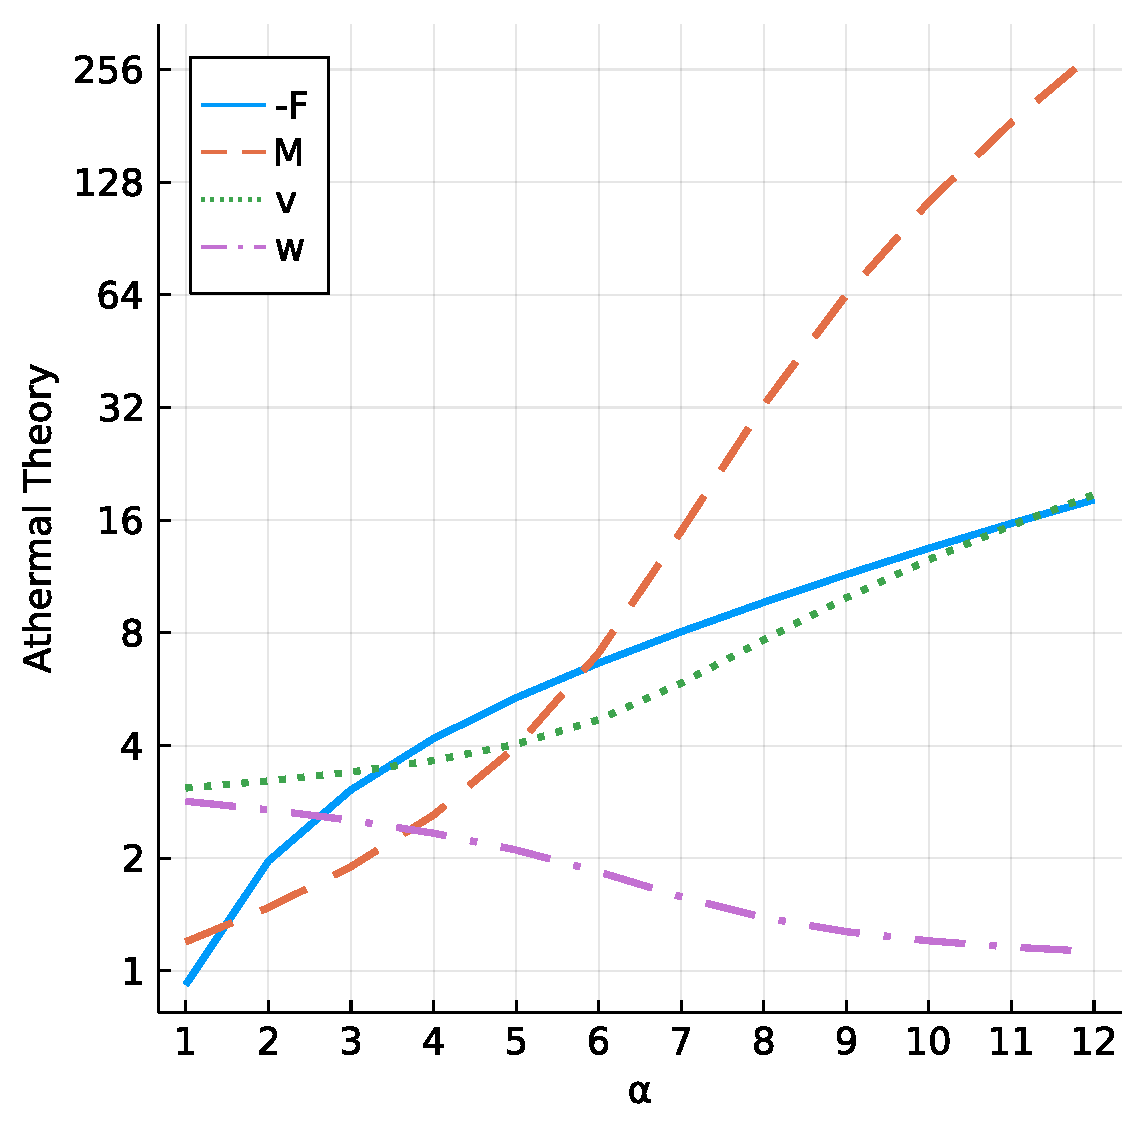
\includegraphics[width=.9\textwidth]{chapters/frohlich/figures/athermal_theory.pdf}
\end{subfigure}%
\begin{subfigure}[b]{.6\textwidth}
\centering
\includegraphics[width=.9\textwidth]{chapters/frohlich/figures/zero_temp_alpha.pdf}
\end{subfigure}%
}
\caption{(left): Unitless values from Feynman's athermal $0$K polaron theory, calculated for electron-phonon $\alpha$ couplings ranging from $1$ to $12$. Blue-solid is the negative of the best approximated ground-state energy $F$, orange-dashed is the polaron effective mass $m_b$, green-dotted is the $v$ variational parameter and purple-dash-dotted is the $w$ variational parameter. (right): The real conductivity (also the frequency-dependent mobility) of the polaron response obtained from the FHIP theory and calculated for $\alpha$ ranging from $1$ to $12$ and external field angular frequencies ranging from $0\ \omega_{LO}$ to $20\ \omega_{LO}$ multiples of the effective phonon angular frequency. The relative magnitudes of the curves for different values of $\alpha$ have been normalised and are not comparable.}
\label{fig:athermaltheory}
\end{figure}

Feynman's original path integral theory (\cite{feynman_slow_1955}) for the polaron produced a variational principle for the ground-state energy of the polaron. The variational $v$ and $w$ parameters that produce the best lower upper-bound to the ground-state energy are then used in expressions that Feynman derived for the polaron effective mass and complex conductivity. 

Figure \ref{fig:athermaltheory}a shows the values of the polaron ground-state energy $-E_{gs}$, effective mass $m_p$ and the corresponding $v$ and $w$, for values of the Fr\"ohlich $\alpha$ parameter ranging from $1$ to $12$. These data are all presented in their `polaron units' form for easier comparison to Feynman's original paper. The ground-state demonstrates the linear weak-coupling behaviour at smaller $\alpha$ before it becomes exponentially more negative as $\alpha$ increases (as the electron-phonon coupling strengthens). The effective mass starts as roughly equal to the conduction electron band-mass $m_p = m_b $ at small $\alpha$ and then becomes exponentially larger at stronger couplings. The $v$ and $w$ variational parameters start off as approximately equal with $v \approx w \approx 3$ at weak couplings, but diverge at strong couplings as $w$ asymptotically approaches $w = 1$ and $v$ increases exponentially at a similar rate to the ground-state energy. 

Figure \ref{fig:athermaltheory}b shows the athermal real conductivity (which is equivalent to the frequency-dependent polaron mobility) for $0 \leq \alpha \leq 12$ and for an applied electric field with an angular frequency $\Omega$ ranging from $0$ to $20$ times that of the longitudinal optical phonon frequency $\omega_{LO}$. At lower couplings $\alpha \leq 4$, all of the first peaks start at $\Omega = \omega_{LO}$ and for $\alpha \geq 5$ we see the appearance of additional peaks at $\Omega = \omega_{LO} + n \omega_{LO} v,\ n \in \mathbb{Z}^+$, with all of the peaks seemingly sharpening and blue-shifting to higher frequencies at stronger couplings $\alpha \geq 7$. However, for very strong couplings $\alpha \geq 10$ the initial peak at $\Omega = \omega_{LO}$ seems to appear again.

\subsection{Thermal theory}

Using \=Osaka's generalised variational principle, I was able to write codes that calculate the polaron free energy, effective mass and complex conductivity for temperatures $T$ ranging from $1$ to $10$ multiples of $\omega_{LO}$ (here $\hbar = k_B = 1$) and for $1\leq\alpha\leq12$. 

In Figure \ref{fig:thermaltheory} are contour plots that show, as a function of temperature $T / \omega_{LO}$ and $\alpha$, (a) the polaron free energy, (b) the polaron effective mass, (c) values of the $v$ variational parameters and (d) values of the $w$ variational parameter. The free energy shows similar behaviour at low temperatures $T \gtrsim \hbar \omega_{LO} / k_B$ to the ground-state energy, but then seems to shift more negative with an increasing negative gradient for $T \gtrsim \hbar \omega_{LO} / k_B$. The effective mass follows a similar pattern as it has a roughly the same behaviour for $T \lesssim \hbar \omega_{LO} / k_B$ as it did for $T = 0$, but becomes exponentially more positive for temperatures $T \gtrsim \hbar \omega_{LO} / k_B$. The $v$ and $w$ parameters also show this pattern and increase exponentially with temperature beyond $T \gtrsim \hbar \omega_{LO} / k_B$. However, $v$ grows faster than $w$ so their difference increases exponentially with temperature too. The artefacts that appear in contour plots for the effective mass and variational parameters at lower $\alpha$ and high temperatures may be numerical error due to difficulties in the optimisation process. The free energy seems to vary less with temperature at weak coupling which may have made finding the global minima difficult, resulting in noise. 

Figure \ref{fig:dcmobility} shows a contour plot of the dc mobility derived in FHIP (note that this expression is unitless). For temperatures $T \lesssim \hbar \omega_{LO} / 2 k_B$ the dc mobility has a minimum around $\alpha \approx 7$ which shifts to larger values of $\alpha$ as the temperature increases. Similarly, for $\alpha \geq 7$ the mobility seems to be minimum around temperatures $T \approx \hbar \omega_{LO} / k_B$. Elsewhere, for $\alpha < 7$ the mobility seems to decrease rapidly as the temperature increases from $0$K up until $T \approx \hbar \omega_{LO} / k_B$, then above this temperature it decreases asymptotically towards zero.

\begin{figure}
\vspace*{-1.5cm}\makebox[\linewidth][c]{%
\begin{subfigure}[t]{0.01\textwidth}
    \vspace*{-7.5cm}\textbf{a}
  \end{subfigure}%
\begin{subfigure}[b]{.6\textwidth}
\centering
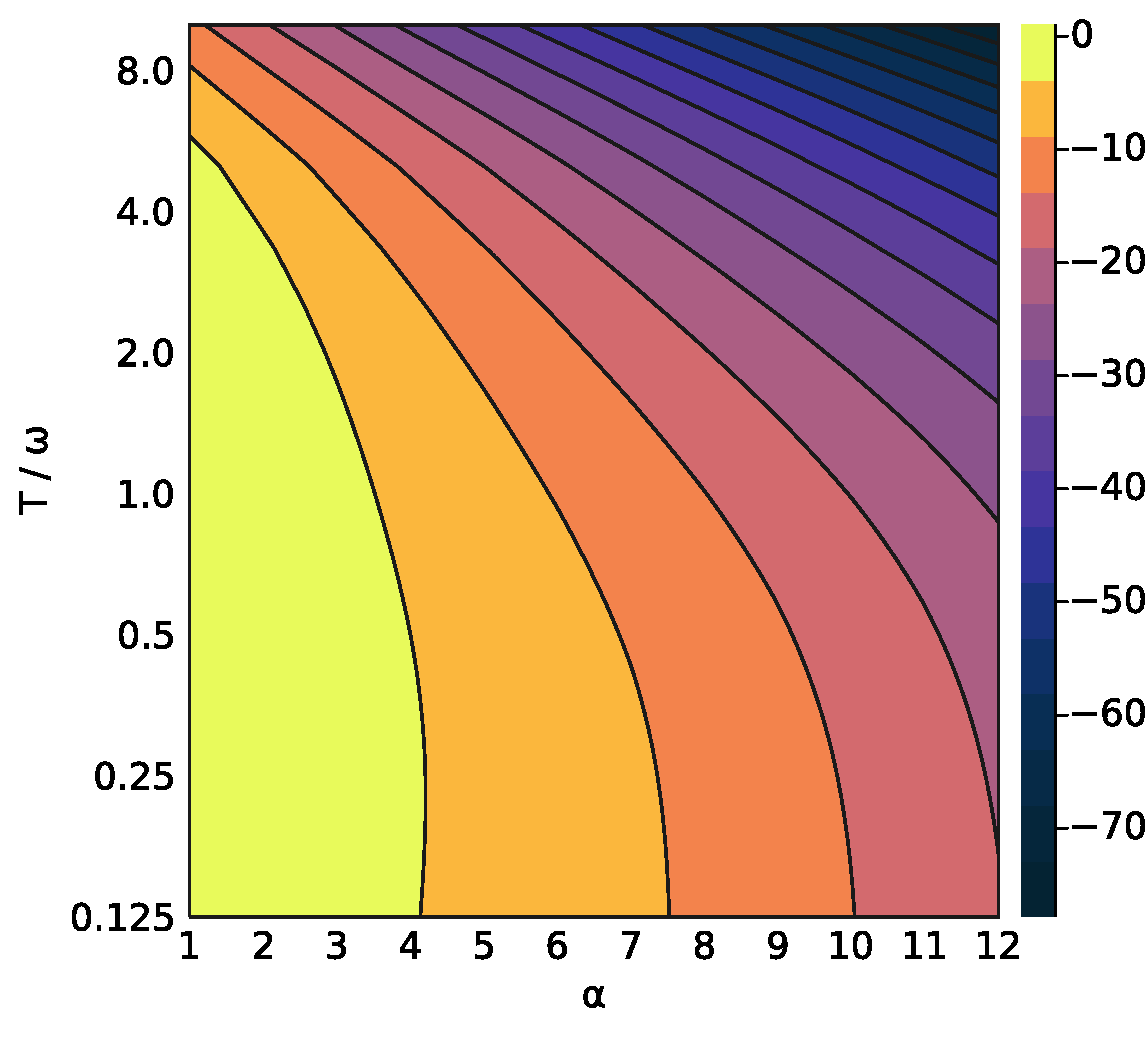
\includegraphics[width=.95\textwidth]{chapters/frohlich/figures/free_energy.pdf}
\end{subfigure}%
\begin{subfigure}[t]{0.01\textwidth}
    \vspace*{-7.5cm}\textbf{b}
  \end{subfigure}
\begin{subfigure}[b]{.6\textwidth}
\centering
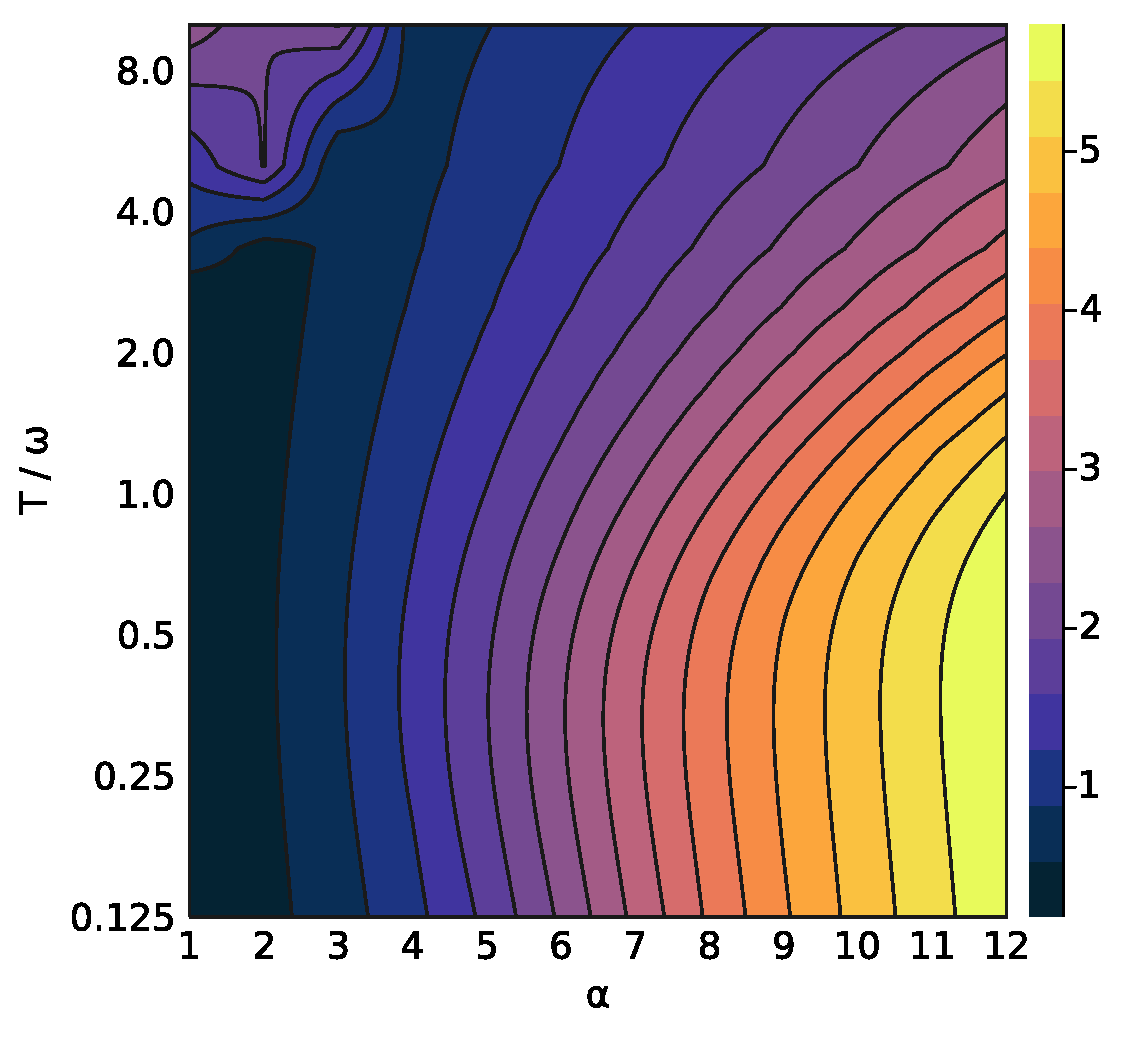
\includegraphics[width=.95\textwidth]{chapters/frohlich/figures/effective_mass.pdf}
\end{subfigure}%
}\\
\makebox[\linewidth][c]{%
\begin{subfigure}[t]{0.01\textwidth}
    \vspace*{-7.5cm}\textbf{c}
  \end{subfigure}%
\begin{subfigure}[b]{.6\textwidth}
\centering
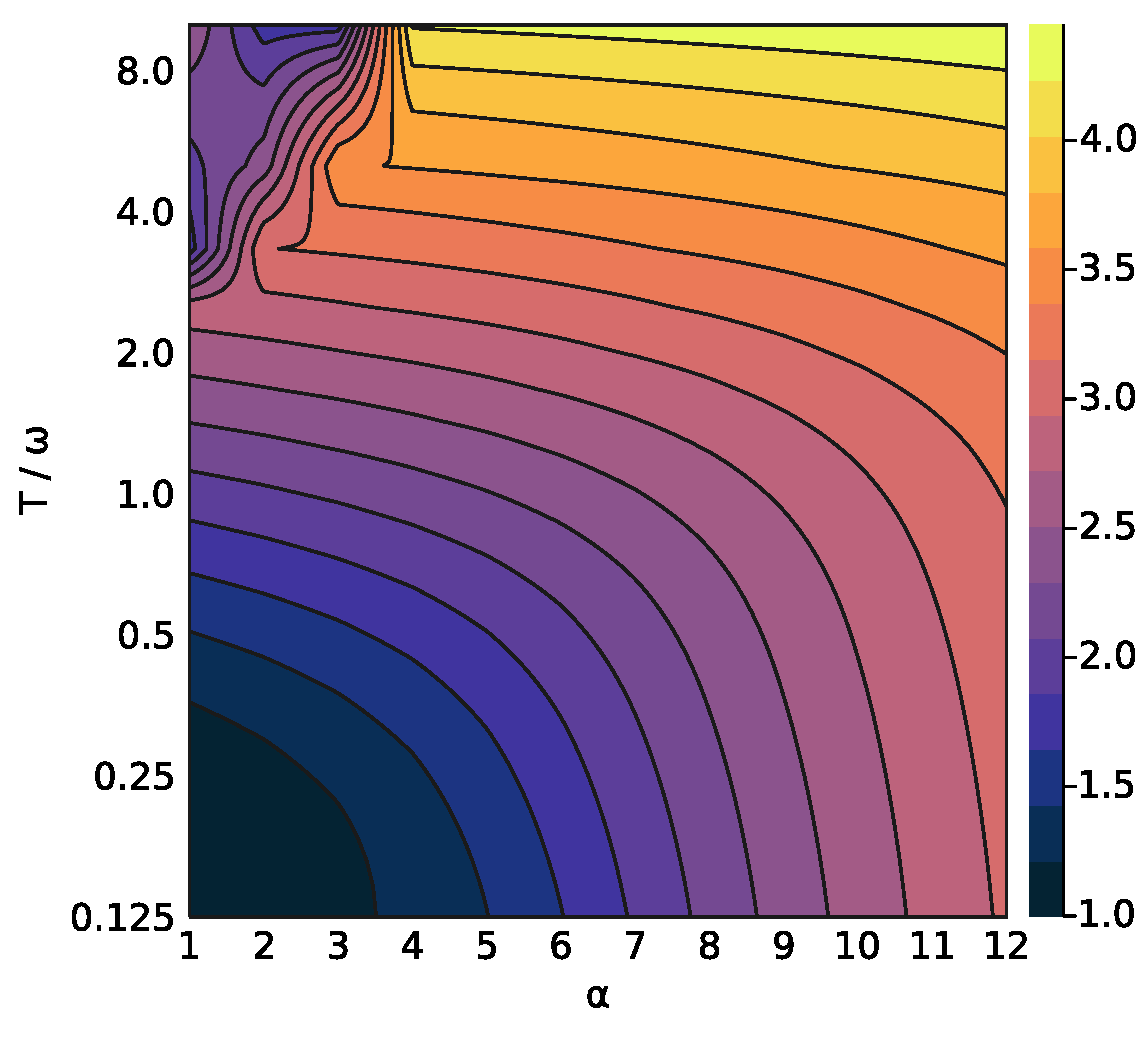
\includegraphics[width=.95\textwidth]{chapters/frohlich/figures/v_parameter.pdf}
\end{subfigure}%
\begin{subfigure}[t]{0.01\textwidth}
    \vspace*{-7.5cm}\textbf{d}
  \end{subfigure}%
\begin{subfigure}[b]{.6\textwidth}
\centering
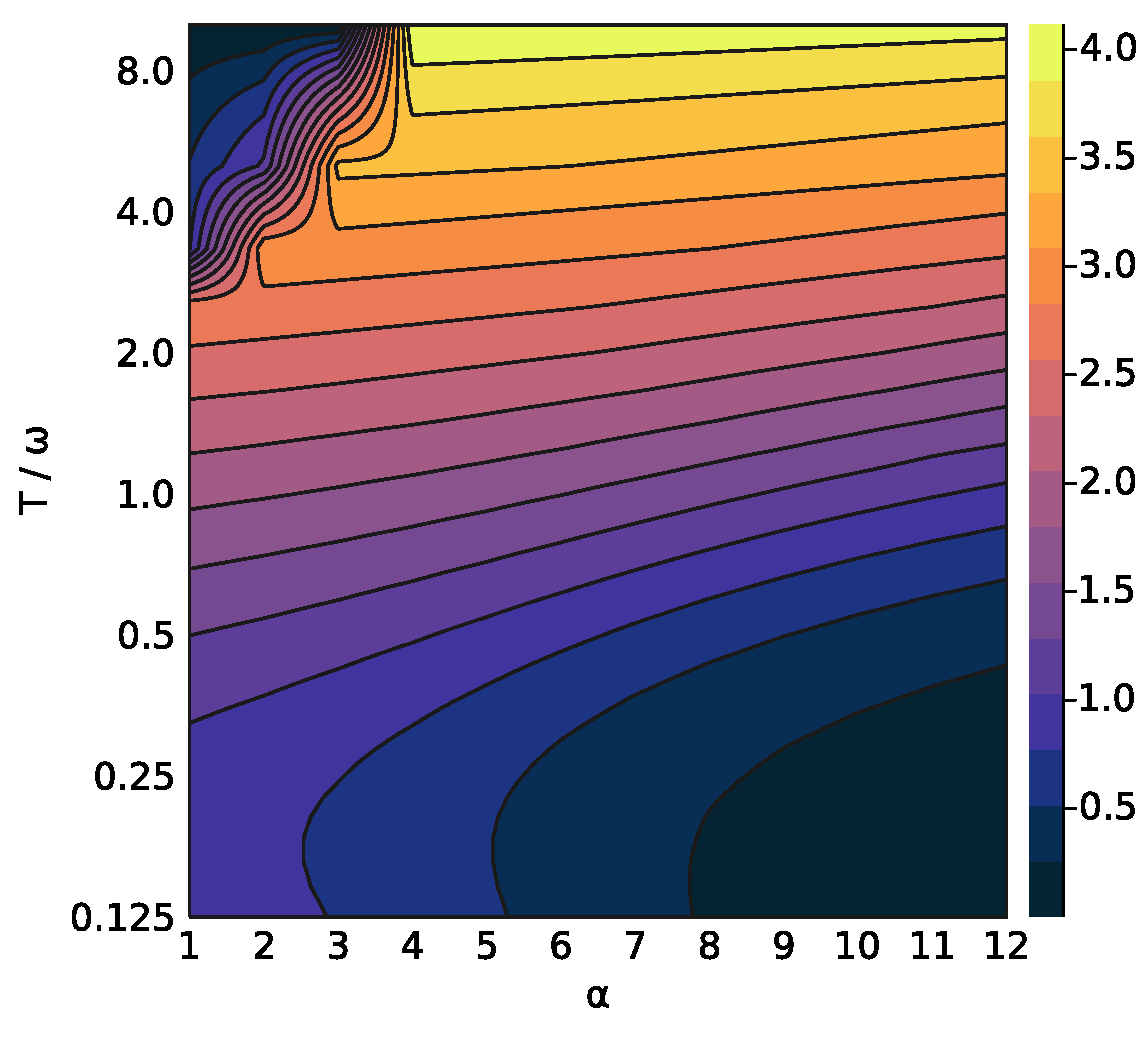
\includegraphics[width=.95\textwidth]{chapters/frohlich/figures/w_parameter.pdf}
\end{subfigure}%
}
\caption{Contour plots of (a) \=Osaka's polaron free energy, (b) Feynman's effective mass (log scale), (c) the $v$ variational parameter (log scale) and (d) the $w$ varational parameter (log scale), as a function of `effective' temperature $T / \omega_{LO}$ and the Fr\"ohlich $\alpha$ parameter.}
\label{fig:thermaltheory}
\end{figure}

\subsection{Optical absorption and complex conductivity}

\begin{figure}
\vspace*{-1.6cm}
\makebox[\linewidth][c]{%
\begin{subfigure}[b]{.65\textwidth}
\centering
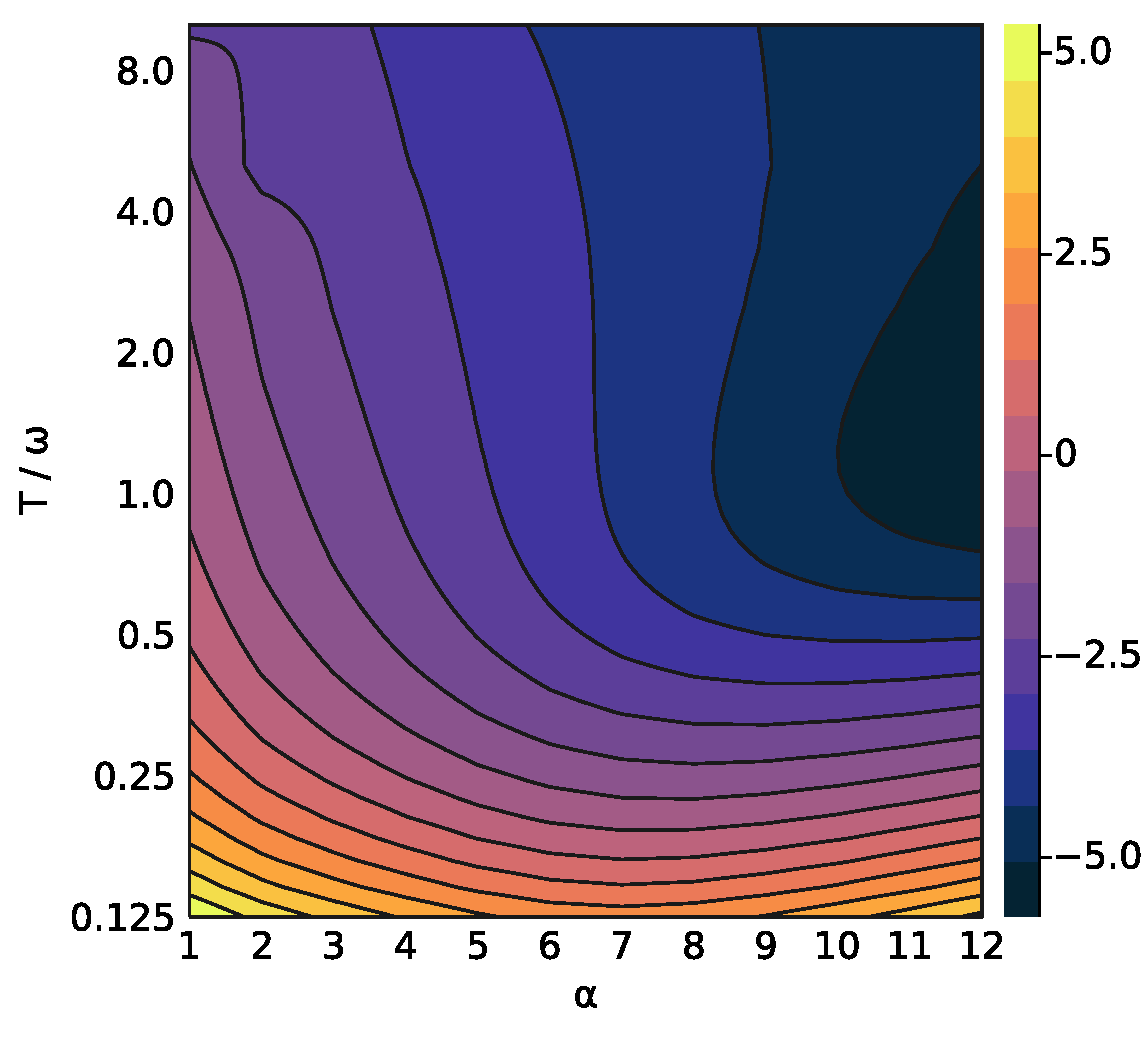
\includegraphics[width=1\textwidth]{chapters/frohlich/figures/dc_mobility.pdf}
\end{subfigure}
}
\caption{Log contour plot of the dc mobility (arbitrary units).}
\label{fig:dcmobility}
\end{figure}

I used the optical absorption expression obtained from~\cite{devreese_optical_1972} to extend the codes to calculate the complex conductivity of the polaron for different couplings $1 \leq \alpha \leq 12$, temperatures $0 \leq T / \omega_{LO} \leq 10$ and applied electric field frequencies $0 \leq \Omega / \omega_{LO} \leq 20$. I show the data obtained for $\alpha = 3, 6, 9$ where perturbation theory breaks down at $\alpha = 6$. 

Figures \ref{fig:osakacontour} (contour plots) and \ref{fig:osakaridge} (ridge-line plots) show the real (left columns) and imaginary (right columns) of the complex conductivity for $\alpha = 3$ in the first rows, $\alpha = 6$ in the second rows and $\alpha = 9$ in the last rows. The figures are all log-scaled with respect to the complex conductivity, and for the imaginary component I have taken the absolute value in order to go to the log-scale. This means that for the imaginary plots, any sharp `rifts' indicate a change in sign as the imaginary component passes through zero. The imaginary component always starts negative at low temperature and frequency, so the first rift can be assumed to indicate a change to a positive sign and so on. I chose $\alpha = 3, 6, 9$ to give some spread of coupling strength about $\alpha = 6$ where perturbation theory typically breaks down. 

From Figures \ref{fig:osakacontour} and \ref{fig:osakaridge} we can see that firstly, at $\alpha = 3$ the complex conductivity starts with a single peak starting at $\Omega = \omega_{LO}$ for zero temperature, which broadens out and blue-shifts to higher frequencies as the temperature increases. This peak corresponds to a single phonon excitation. At $\alpha = 6$ the conductivity develops more peaks starting at $\Omega = \omega_{LO} + n \omega_{LO} v,\ n \in \mathbb{Z}^+$ at zero temperature, corresponding to further phonon excitations, which also broaden out and blue-shift to higher frequencies as the temperature increases. The first peak for $\alpha = 6$ now has more features, with an initial shoulder which leads into a far sharper peak than before, and sharper, more structured peaks as $\alpha$ increases. Finally, for $\alpha = 9$ the landscape becomes much more erratic and complex. The first peak still remains, however the trough that follows it has become so deep (reaching values close to zero) that the numerical results is noisy due to reaching float-point accuracy (working here with 64-bit floats). The second main peak (that I identify as regions now separated by the deep troughs) now seems to begin a little earlier than $\Omega = \omega_{LO} + v \omega_{LO}$ and appears to be composed of smaller, sharper peaks and shoulders. 

\begin{figure}[h]
\vspace*{-1.5cm}\makebox[\linewidth][c]{%
\begin{subfigure}[t]{0.01\textwidth}
    \vspace*{-8.2cm}\hspace*{9.4cm}\textbf{$\vb{\alpha}$=3}
    \vspace*{-7.5cm}\textbf{a}
  \end{subfigure}%
\begin{subfigure}[b]{.6\textwidth}
\centering
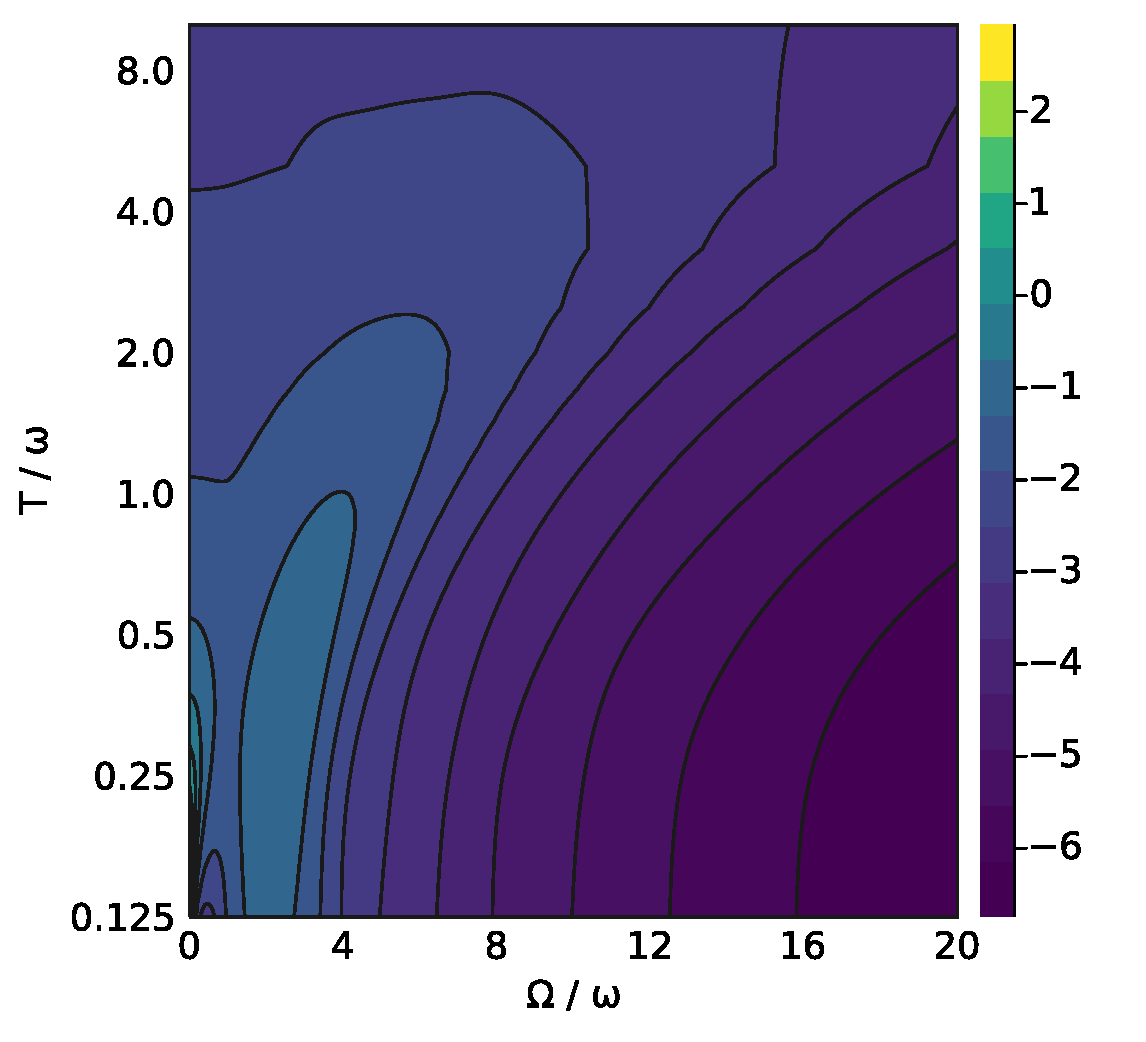
\includegraphics[width=.92\textwidth]{chapters/frohlich/figures/conductivity_contour_real_3.pdf}
\end{subfigure}%
\begin{subfigure}[t]{0.01\textwidth}
    \vspace*{-7.5cm}\textbf{b}
  \end{subfigure}
\begin{subfigure}[b]{.6\textwidth}
\centering
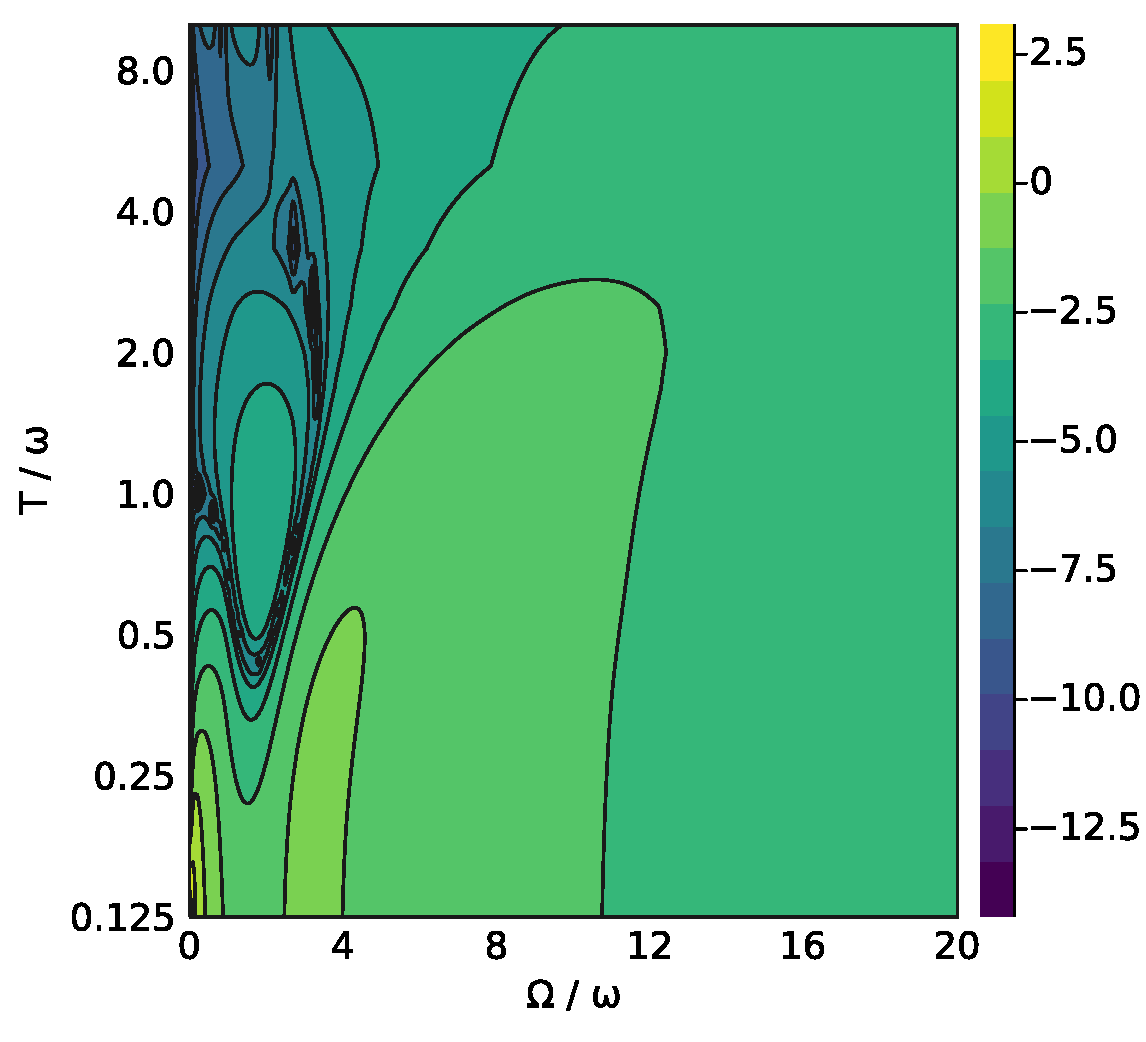
\includegraphics[width=.92\textwidth]{chapters/frohlich/figures/conductivity_contour_imag_3.pdf}
\end{subfigure}%
}\\
\makebox[\linewidth][c]{%
\begin{subfigure}[t]{0.01\textwidth}
    \vspace*{-8.2cm}\hspace*{9.4cm}\textbf{$\vb{\alpha}$=6}
    \vspace*{-7.5cm}\textbf{c}
  \end{subfigure}%
\begin{subfigure}[b]{.6\textwidth}
\centering
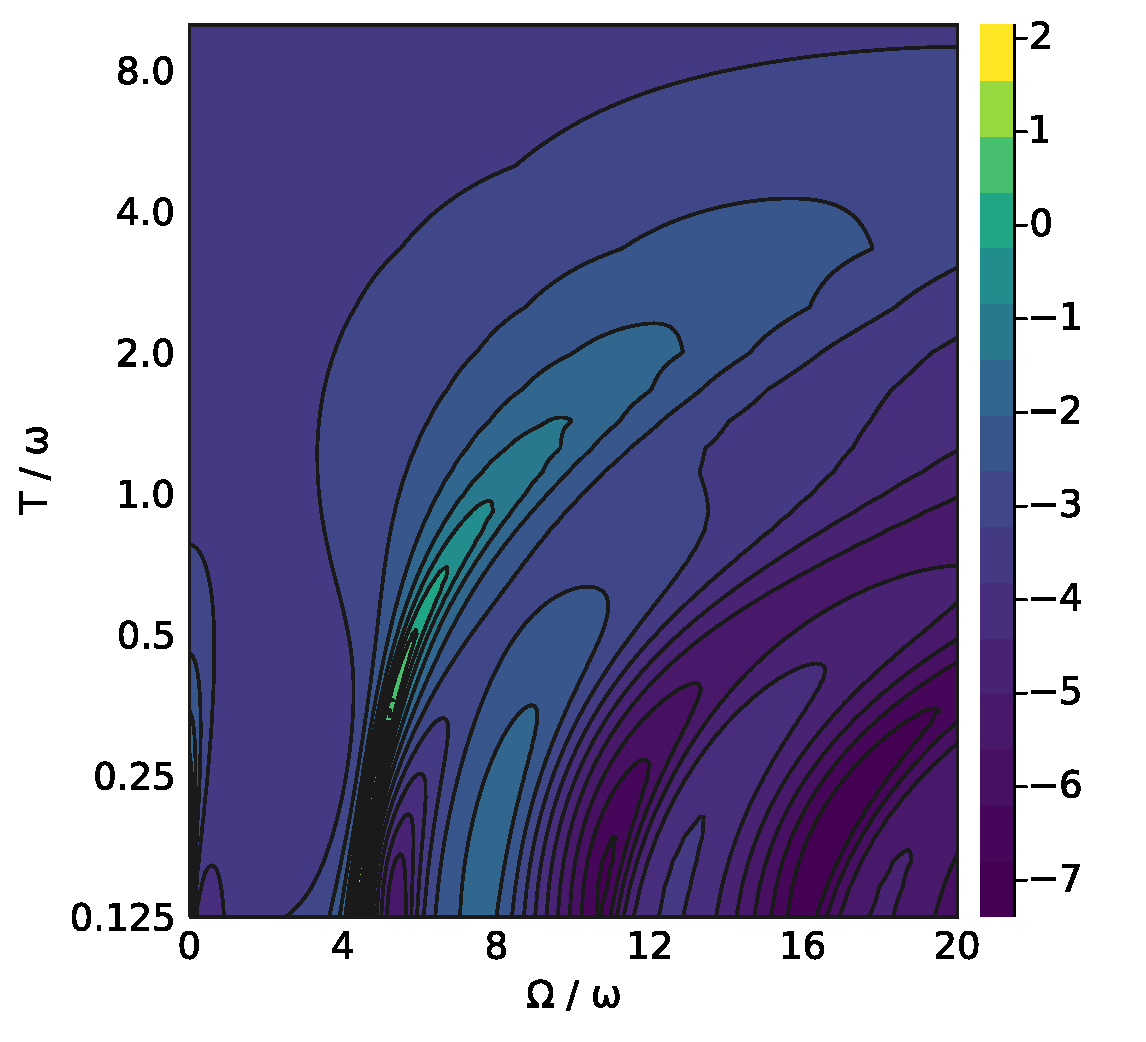
\includegraphics[width=.92\textwidth]{chapters/frohlich/figures/conductivity_contour_real_6.pdf}
\end{subfigure}%
\begin{subfigure}[t]{0.01\textwidth}
    \vspace*{-7.5cm}\textbf{d}
  \end{subfigure}%
\begin{subfigure}[b]{.6\textwidth}
\centering
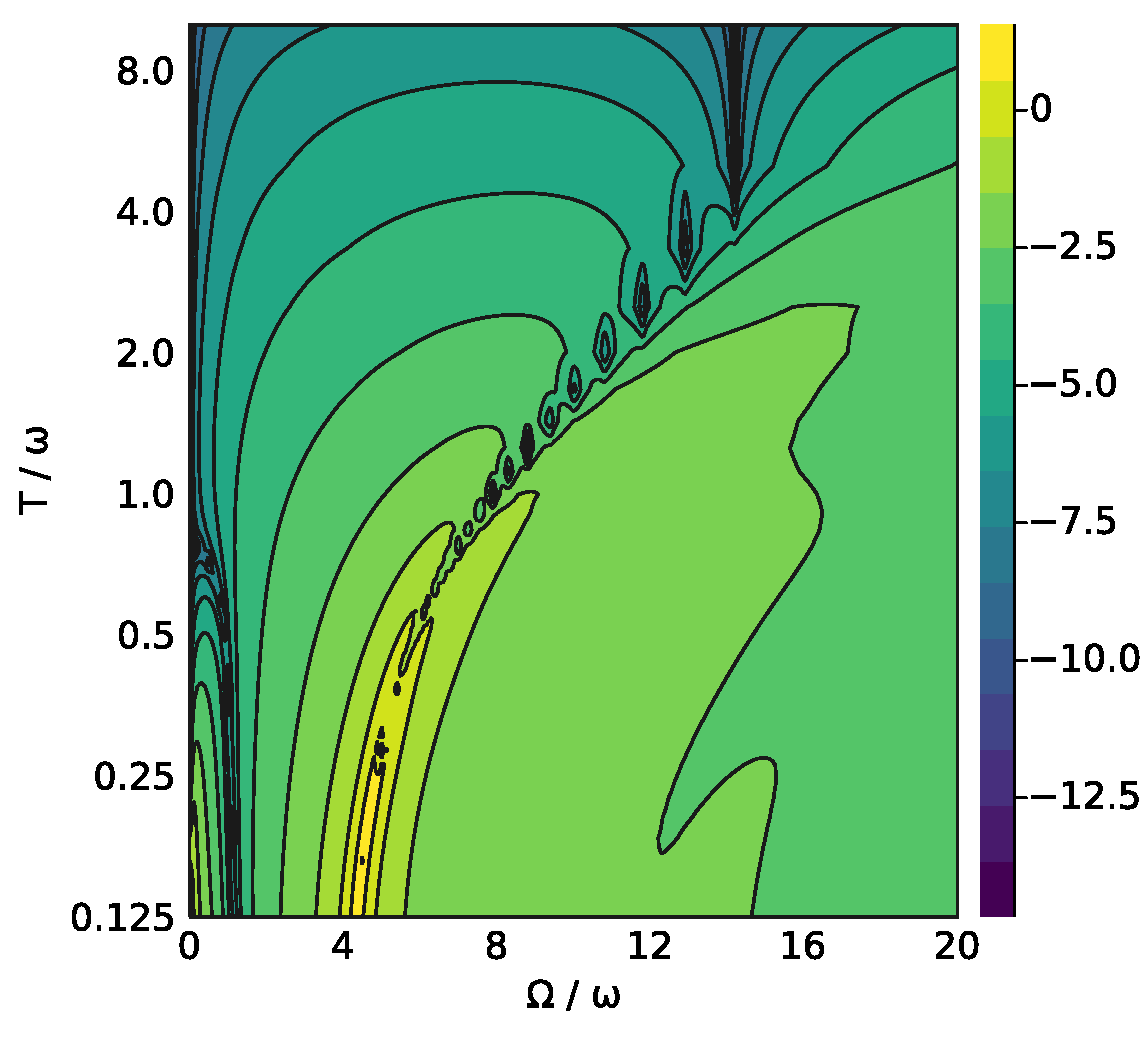
\includegraphics[width=.92\textwidth]{chapters/frohlich/figures/conductivity_contour_imag_6.pdf}
\end{subfigure}%
}
\makebox[\linewidth][c]{%
\begin{subfigure}[t]{0.01\textwidth}
    \vspace*{-8.2cm}\hspace*{9.4cm}\textbf{$\vb{\alpha}$=9}
    \vspace*{-7.5cm}\textbf{e}
  \end{subfigure}%
\begin{subfigure}[b]{.6\textwidth}
\centering
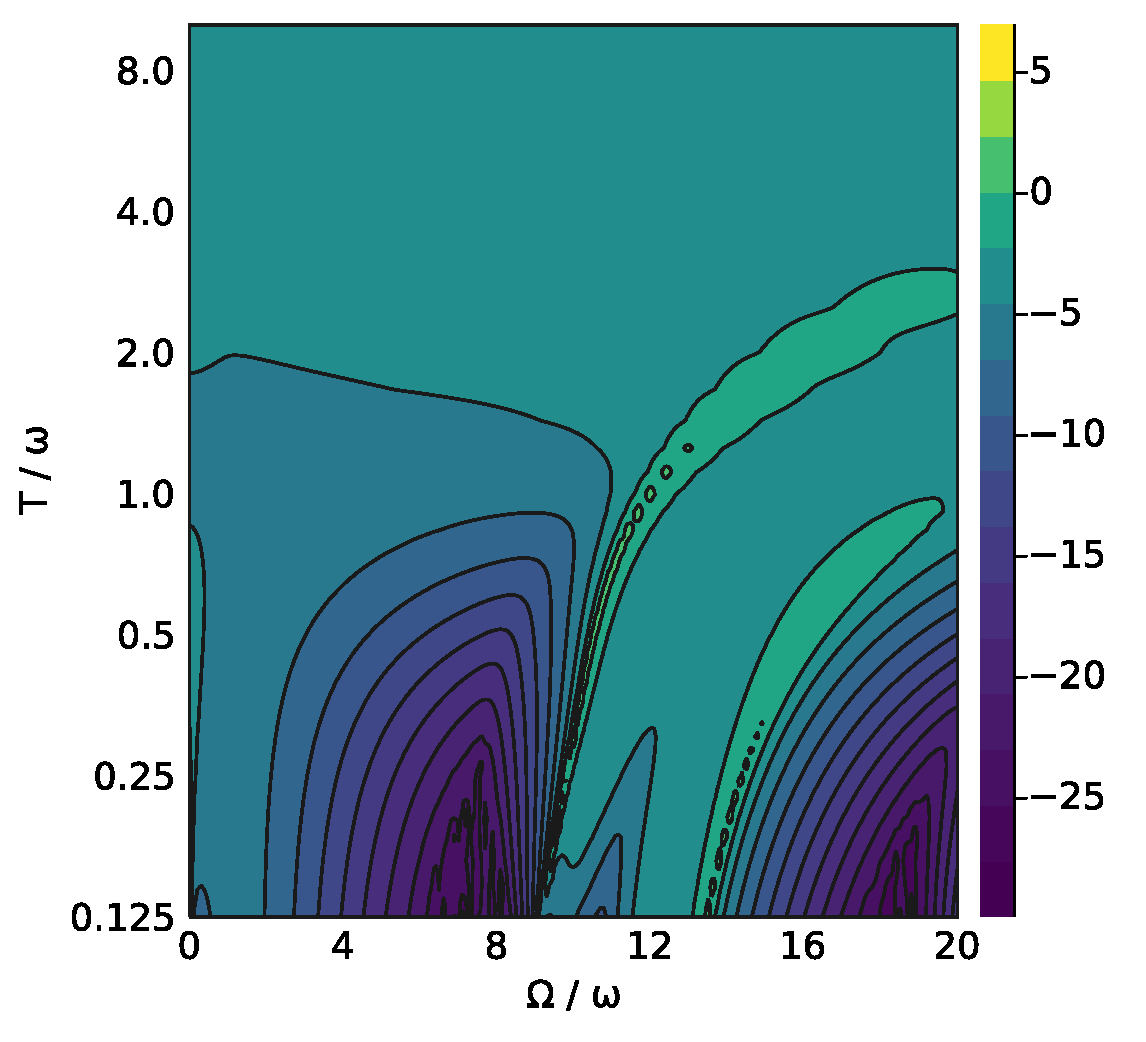
\includegraphics[width=.92\textwidth]{chapters/frohlich/figures/conductivity_contour_real_9.pdf}
\end{subfigure}%
\begin{subfigure}[t]{0.01\textwidth}
    \vspace*{-7.5cm}\textbf{f}
  \end{subfigure}%
\begin{subfigure}[b]{.6\textwidth}
\centering
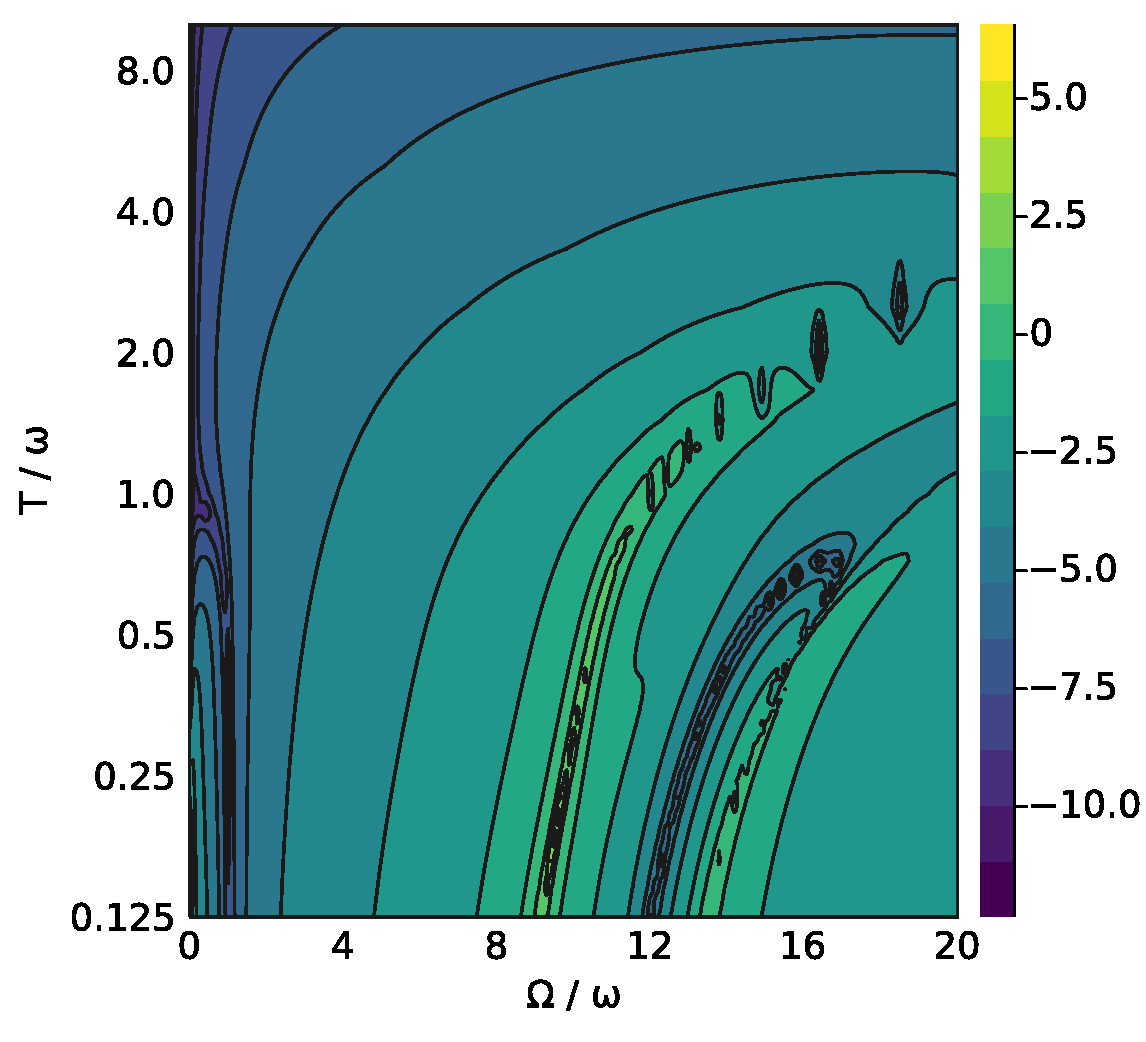
\includegraphics[width=.92\textwidth]{chapters/frohlich/figures/conductivity_contour_imag_9.pdf}
\end{subfigure}%
}
\caption{Contours for the real (left) and imaginary (right) complex conductivity at different values of $\alpha$. (a) Real conductivity at $\alpha = 3$. (b) Imaginary conductivity at $\alpha = 3$. (c) Real conductivity at $\alpha = 6$. (d) Imaginary conductivity at $\alpha = 6$. (e) Real conductivity at $\alpha = 9$. (f) Imaginary conductivity at $\alpha = 9$.}
\label{fig:osakacontour}
\end{figure}

\begin{figure}[h]
\vspace*{-1.5cm}\makebox[\linewidth][c]{%
\begin{subfigure}[t]{0.01\textwidth}
    \vspace*{-8.2cm}\hspace*{9.2cm}\textbf{\underline{$\vb{\alpha}$=3}}
    \vspace*{-7.5cm}\textbf{a}
  \end{subfigure}%
\begin{subfigure}[b]{.58\textwidth}
\centering
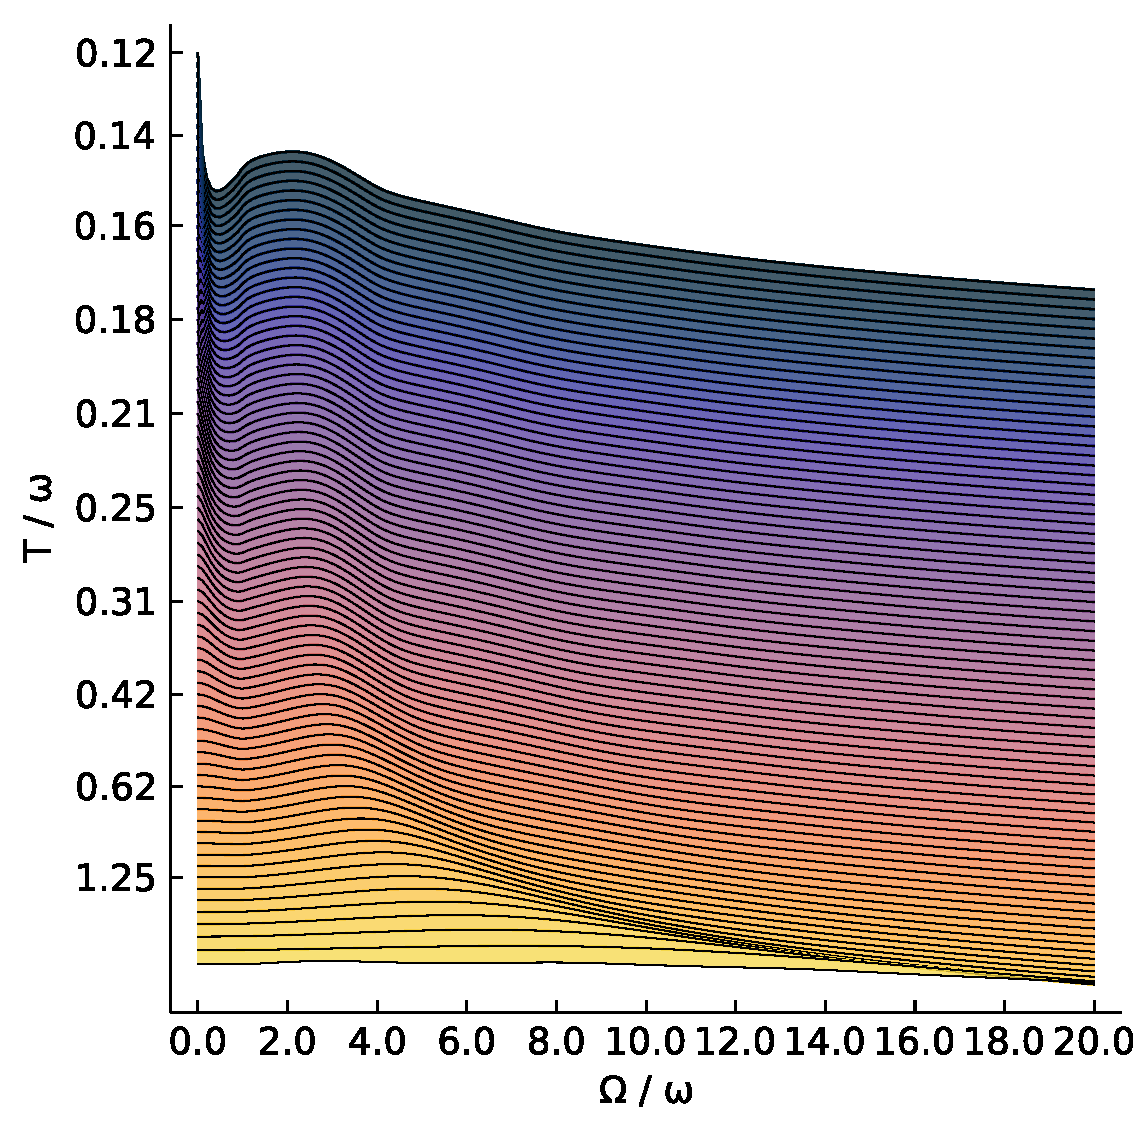
\includegraphics[width=.87\textwidth]{chapters/frohlich/figures/conductivity_plot_temp_real_3.pdf}
\end{subfigure}%
\begin{subfigure}[t]{0.01\textwidth}
    \vspace*{-7.5cm}\textbf{b}
  \end{subfigure}
\begin{subfigure}[b]{.58\textwidth}
\centering
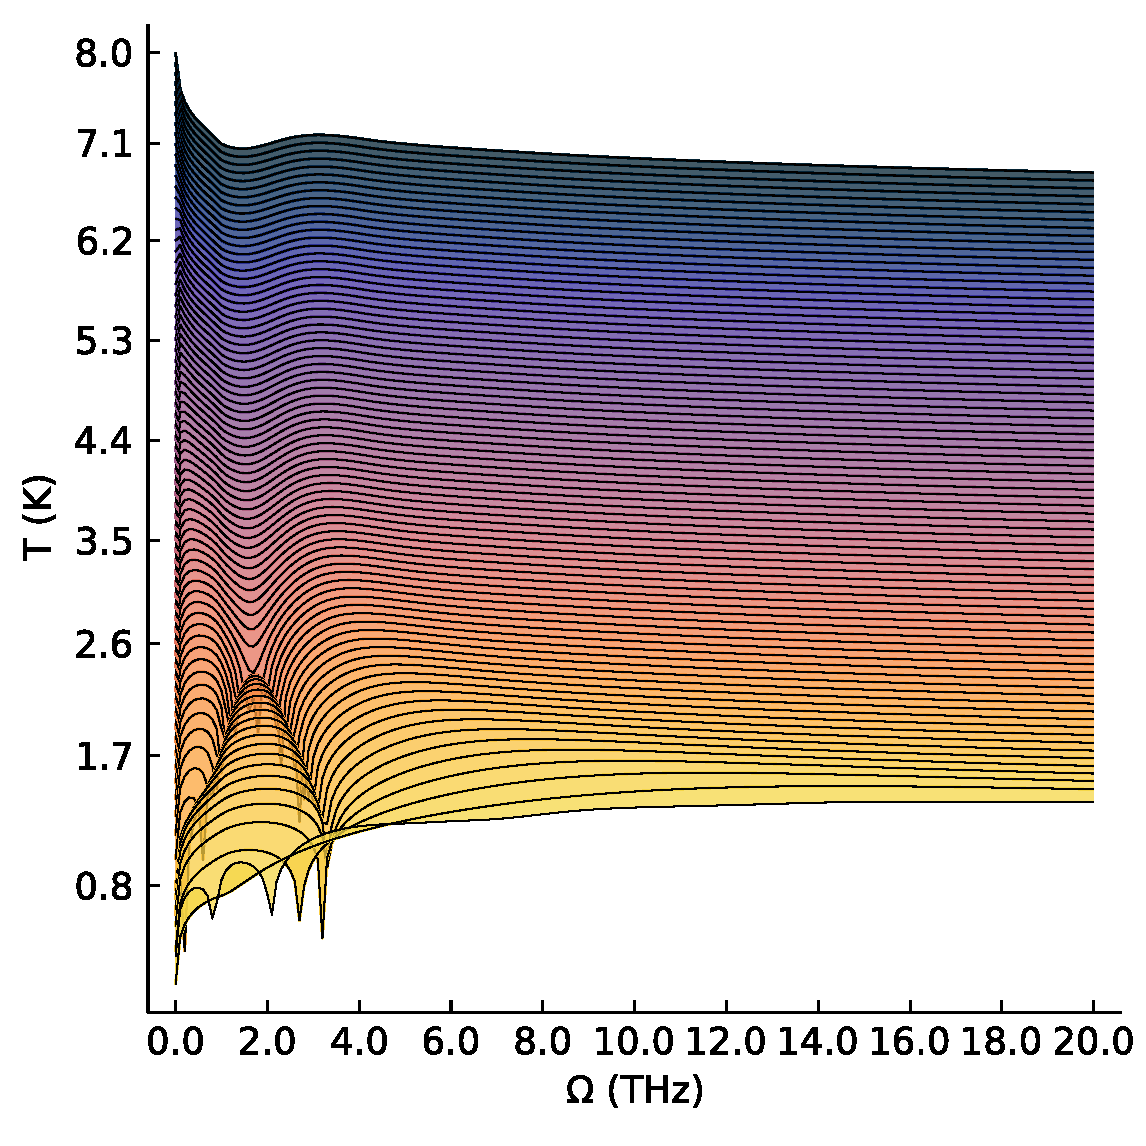
\includegraphics[width=.87\textwidth]{chapters/frohlich/figures/conductivity_plot_temp_imag_3.pdf}
\end{subfigure}%
}\\
\makebox[\linewidth][c]{%
\begin{subfigure}[t]{0.01\textwidth}
    \vspace*{-8.2cm}\hspace*{9.2cm}\textbf{\underline{$\vb{\alpha}$=6}}
    \vspace*{-7.5cm}\textbf{c}
  \end{subfigure}%
\begin{subfigure}[b]{.58\textwidth}
\centering
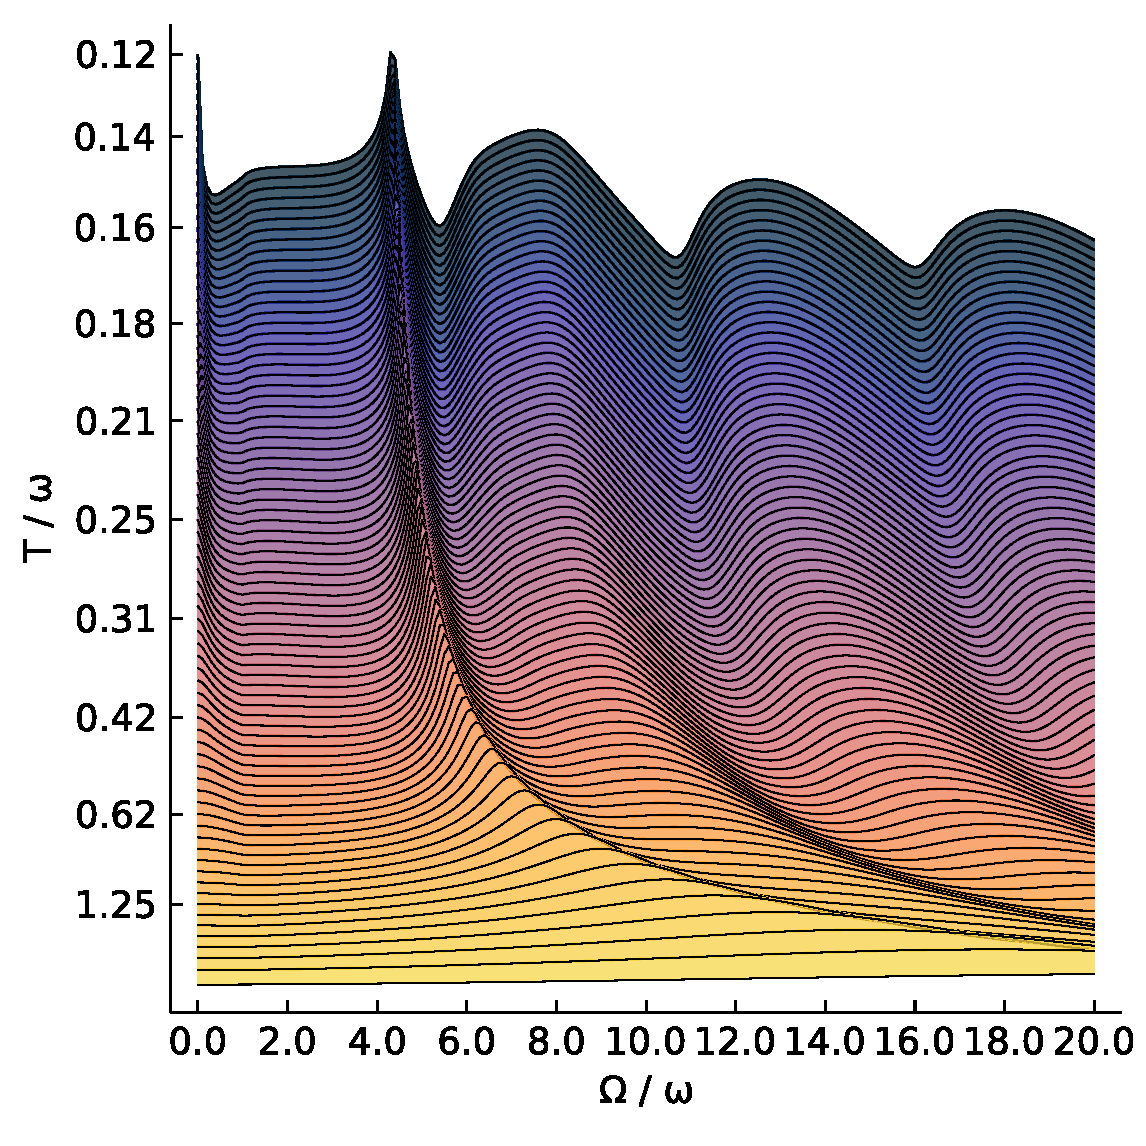
\includegraphics[width=.87\textwidth]{chapters/frohlich/figures/conductivity_plot_temp_real_6.pdf}
\end{subfigure}%
\begin{subfigure}[t]{0.01\textwidth}
    \vspace*{-7.5cm}\textbf{d}
  \end{subfigure}%
\begin{subfigure}[b]{.58\textwidth}
\centering
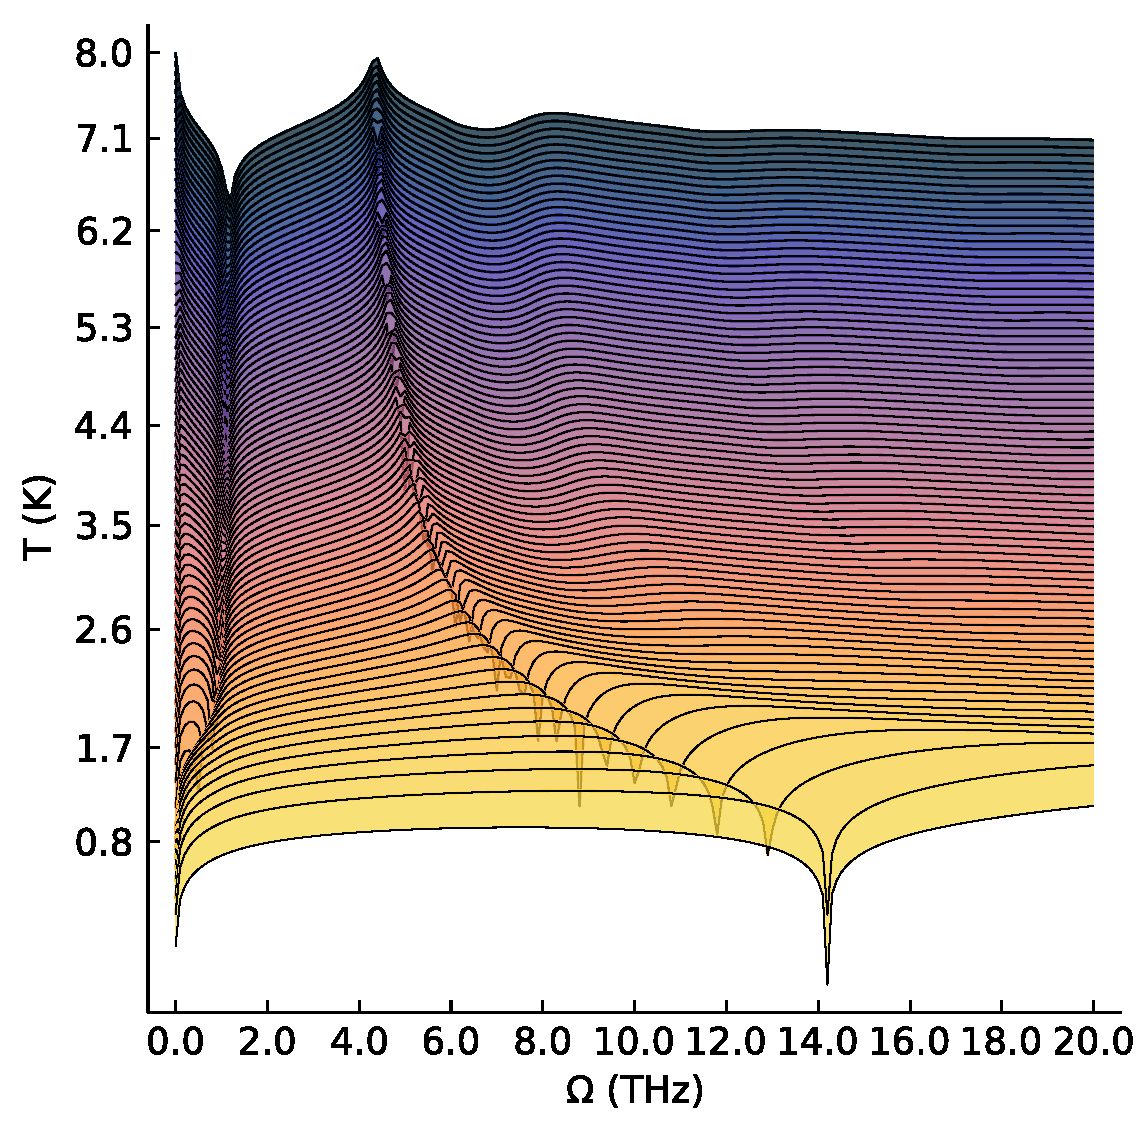
\includegraphics[width=.87\textwidth]{chapters/frohlich/figures/conductivity_plot_temp_imag_6.pdf}
\end{subfigure}%
}
\makebox[\linewidth][c]{%
\begin{subfigure}[t]{0.01\textwidth}
    \vspace*{-8.2cm}\hspace*{9.2cm}\textbf{\underline{$\vb{\alpha}$=9}}
    \vspace*{-7.5cm}\textbf{e}
  \end{subfigure}%
\begin{subfigure}[b]{.58\textwidth}
\centering
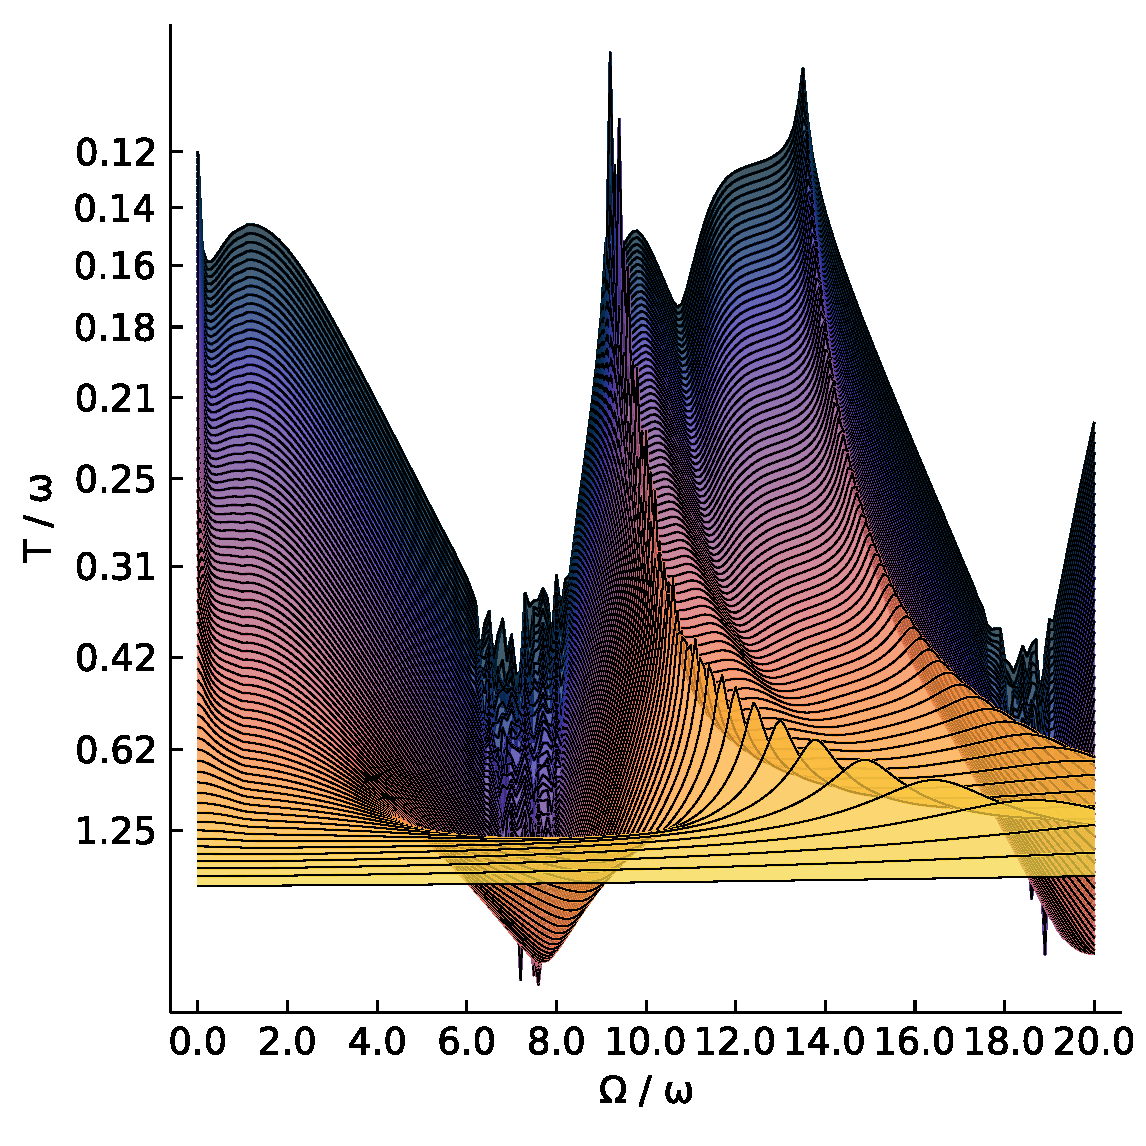
\includegraphics[width=.87\textwidth]{chapters/frohlich/figures/conductivity_plot_temp_real_9.pdf}
\end{subfigure}%
\begin{subfigure}[t]{0.01\textwidth}
    \vspace*{-7.5cm}\textbf{f}
  \end{subfigure}%
\begin{subfigure}[b]{.58\textwidth}
\centering
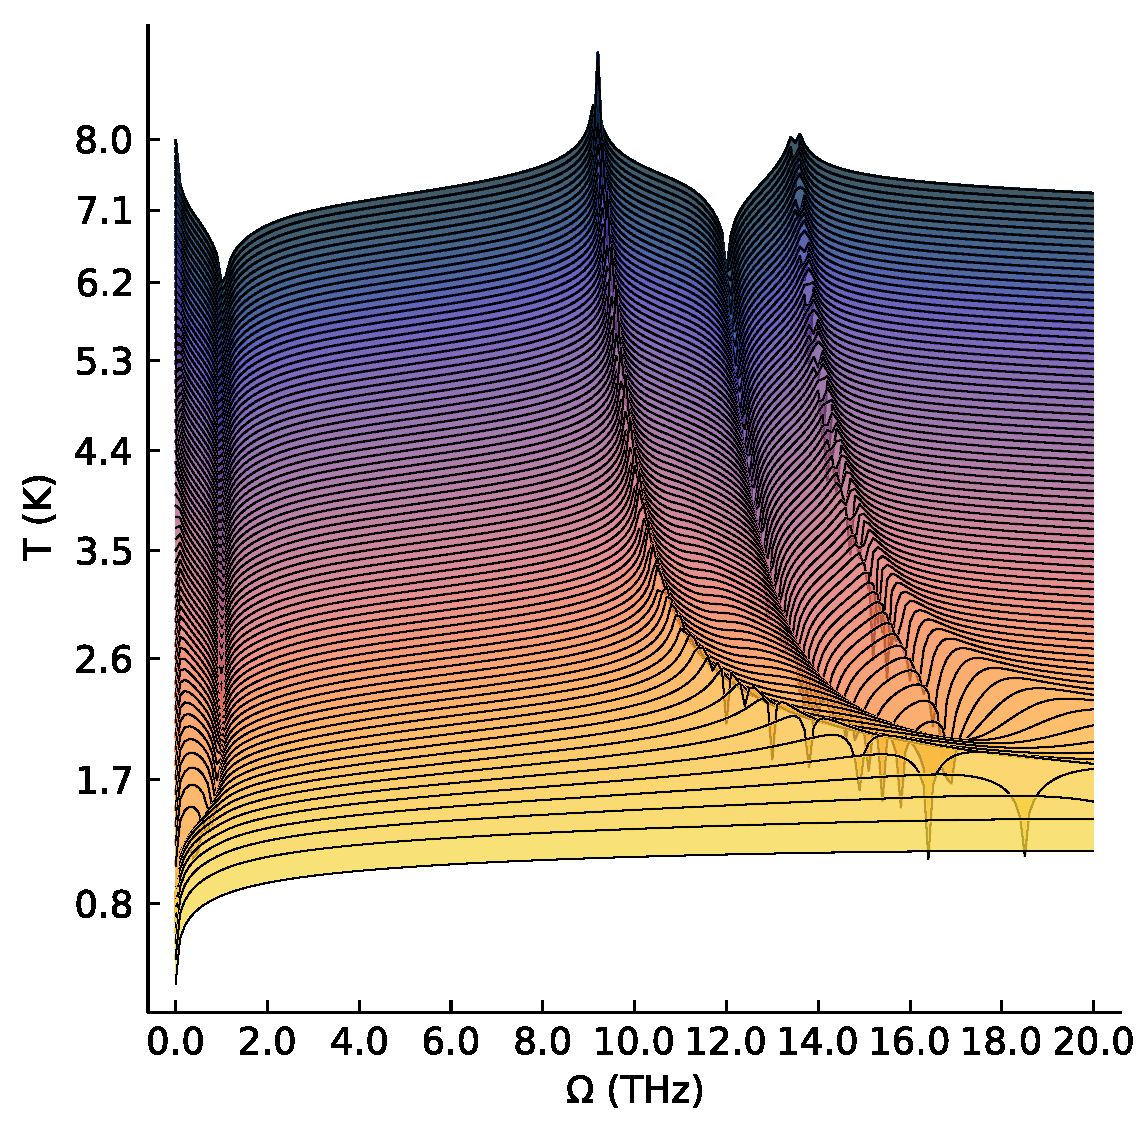
\includegraphics[width=.87\textwidth]{chapters/frohlich/figures/conductivity_plot_temp_imag_9.pdf}
\end{subfigure}%
}
\caption{Ridgeline plots for the real (left) and imaginary (right) complex conductivity at different values of $\alpha$. (a) Real conductivity at $\alpha = 3$. (b) Imaginary conductivity at $\alpha = 3$. (c) Real conductivity at $\alpha = 6$. (d) Imaginary conductivity at $\alpha = 6$. (e) Real conductivity at $\alpha = 9$. (f) Imaginary conductivity at $\alpha = 9$.}
\label{fig:osakaridge}
\end{figure}

\subsection{Polaron mobility in the ``Beyond Quasiparticle'' regime}

\begin{figure}[t]
\vspace*{-1.5cm}\makebox[\linewidth][c]{%
\begin{subfigure}[b]{.6\textwidth}
\centering
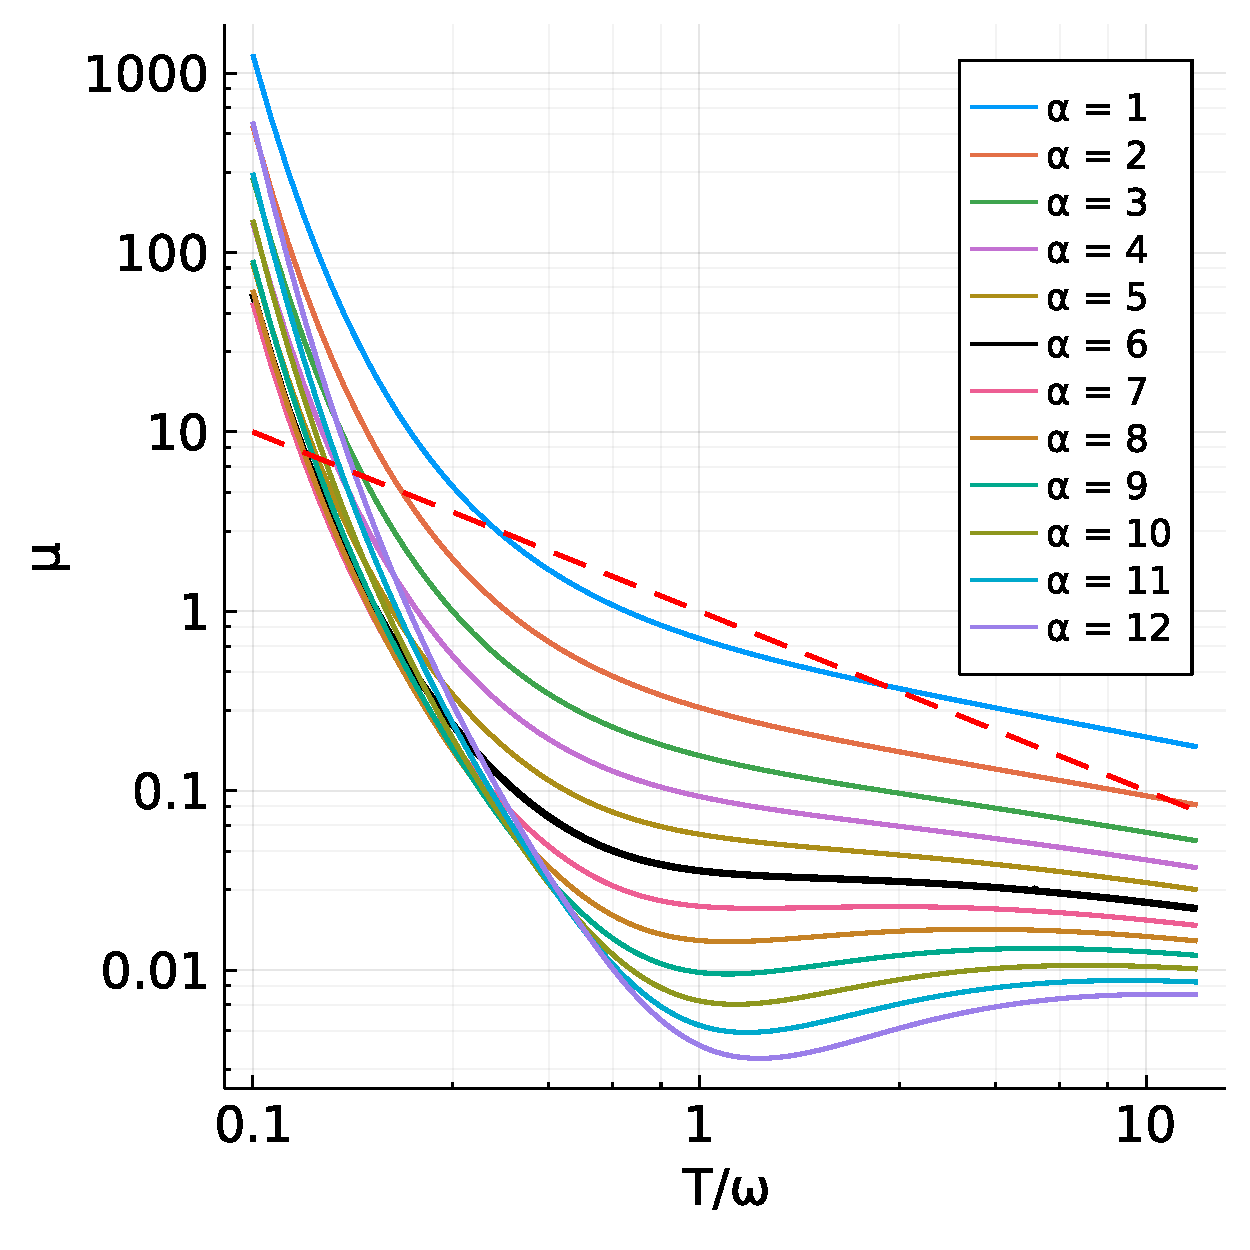
\includegraphics[width=.9\textwidth]{chapters/frohlich/figures/moblility_temp_alpha.pdf}
\end{subfigure}%
\begin{subfigure}[b]{.6\textwidth}
\centering
\includegraphics[width=.9\textwidth]{chapters/frohlich/figures/medium (1).png}
\end{subfigure}%
}
\caption{Temperature dependence of the polaron mobility. The Mott-Ioffe-Regel (MIR) threshold is given by the red dotted lines. Left: Mobility obtained from the thermal FHIP theory with $v$ and $w$ variational parameters calculated for each temperature, for Fr\"ohlich alphas ranging from $\alpha = 1$ to  $12$. The temperature is given in units of the phonon frequency $\omega$. Right: Mobility obtained by~\cite{mishchenko_polaron_2019} using the diagrammatic Monte Carlo method for $\alpha = 6$. The temperature is in units of the phonon frequency $\Omega$.}
\label{fig:mishchenko2}
\end{figure}

\cite{mishchenko_polaron_2019} use the diagrammatic Monte Carlo (DiagMC) method to study the mobility of a Fr\"ohlich polaron in the ``Beyond Quasiparticle'' regime. In this regime, the inelastic scattering rate exceeds the thermal energy of quasiparticles. This can be restated as the regime where the mean free path of the particle exceeds its de Broglie wavelength. In this form, it coincides with the Mott-Ioffe-Regel (MIR) criterion where the motion of quasiparticles is ill-defined. 

In Figure \ref{fig:mishchenko2} are comparisons between the temperature dependence of the polaron mobility evaluated using the~\cite{feynman_mobility_1962} method (right) compared to the~\cite{mishchenko_polaron_2019} DiagMC method (left). The key features of the DiagMC plot (right) are the non-monotonic behaviour of the mobility and the evaluation of the mobility near and below the MIR threshold (given by the red dotted line). These two features are seen in the FHIP mobility too. The main difference between the two results is that, whilst the mobility minimum arises from the DiagMC method at $\alpha = 6$, the minimum arises from the FHIP method at $\alpha \geq 7$ and is less prominent. 

\begin{figure}[t]
\vspace*{-1.5cm}\makebox[\linewidth][c]{%
\begin{subfigure}[b]{.6\textwidth}
\centering
\includegraphics[width=.9\textwidth]{chapters/frohlich/figures/Mischenko_comparison.pdf}
\end{subfigure}%
\begin{subfigure}[b]{.6\textwidth}
\centering
\includegraphics[width=.9\textwidth]{chapters/frohlich/figures/medium.png}
\end{subfigure}%
}
\caption{Polaron mobility for $\alpha = 6$. Left: Mobility obtained from the thermal FHIP theory with $v$ and $w$ variational parameters calculated for each temperature. The electric field frequency and temperature are given in units of the phonon frequency $\omega$. Right: Mobility obtained by~\cite{mishchenko_polaron_2019} using the diagrammatic Monte Carlo method. The electric field frequency and temperature are in units of the phonon frequency $\Omega$.}
\label{fig:mishchenko}
\end{figure}

The mobility evaluated below the MIR threshold is stated in~\cite{mishchenko_polaron_2019} to be ``beyond the quasiparticle'' regime. However, the model from~\cite{feynman_mobility_1962} can reliably evaluate the mobility in this regime too, despite being a quasiparticle model of two fictitious masses coupled by a spring-like potential. Additionally, the FHIP can reproduce the mobility minimum too. \cite{mishchenko_polaron_2019} suggest that the minimum emerges from the competition between the decreasing number of thermal excitations (which dominates for at $T << \omega$) and a strong mass renormalisation (which is prominent for $T \gtrsim \omega$). 

In Figure \ref{fig:mishchenko} are comparisons between the polaron mobility evaluated for a Fr\"ohlich alpha $\alpha = 6$. The left figure shows the polaron mobility obtained from the thermal Feynman polaron theory (evaluated with (Eq. \ref{eqn:FHIP_mobility}) for the dc polaron mobility). The right figure shows the polaron mobility obtained from~\cite{mishchenko_polaron_2019}'s DiagMC method. The position of the peaks between the two methods align for each temperature ($0.125, 0.25, 0.5, 1, 2, 4\  \&\ 8\ K/\omega$, where $\omega$ is the single phonon mode frequency). The main difference between the two methods is that the peaks evaluated from the Feynman polaron method are taller and sharper, whereas the peaks evaluated from~\cite{mishchenko_polaron_2019}'s DiagMC method are broader and shallower. 

The difference in peak widths between the two methods is likely due to the two-mass spring model approximation made in the Feynman method within the trial action in Eq. (\ref{eqn:thermal_trial_action}). This fixes the dynamical behaviour of Feynman's model \emph{a priori} since it only contains two harmonic degrees of freedom. The translation invariance of the Fr\"ohlich Hamiltonian then fixes one eigenmode at zero frequency. The frequency of the other mode and the relative spectral weight of the peaks are then the free parameters. This spectrum differs greatly from the true spectrum of the polaron, and means that the FHIP polaron mobility may only contain a very crude approximation of the true dissipation of the polaron. The dynamical properties of the FHIP approximation is investigated more by~\cite{sels_dynamic_2016}.

\begin{figure}
\vspace*{-1.5cm}\makebox[\linewidth][c]{%
\begin{subfigure}[t]{0.01\textwidth}
    \vspace*{-7.5cm}\textbf{a}
  \end{subfigure}%
\begin{subfigure}[b]{.58\textwidth}
\centering
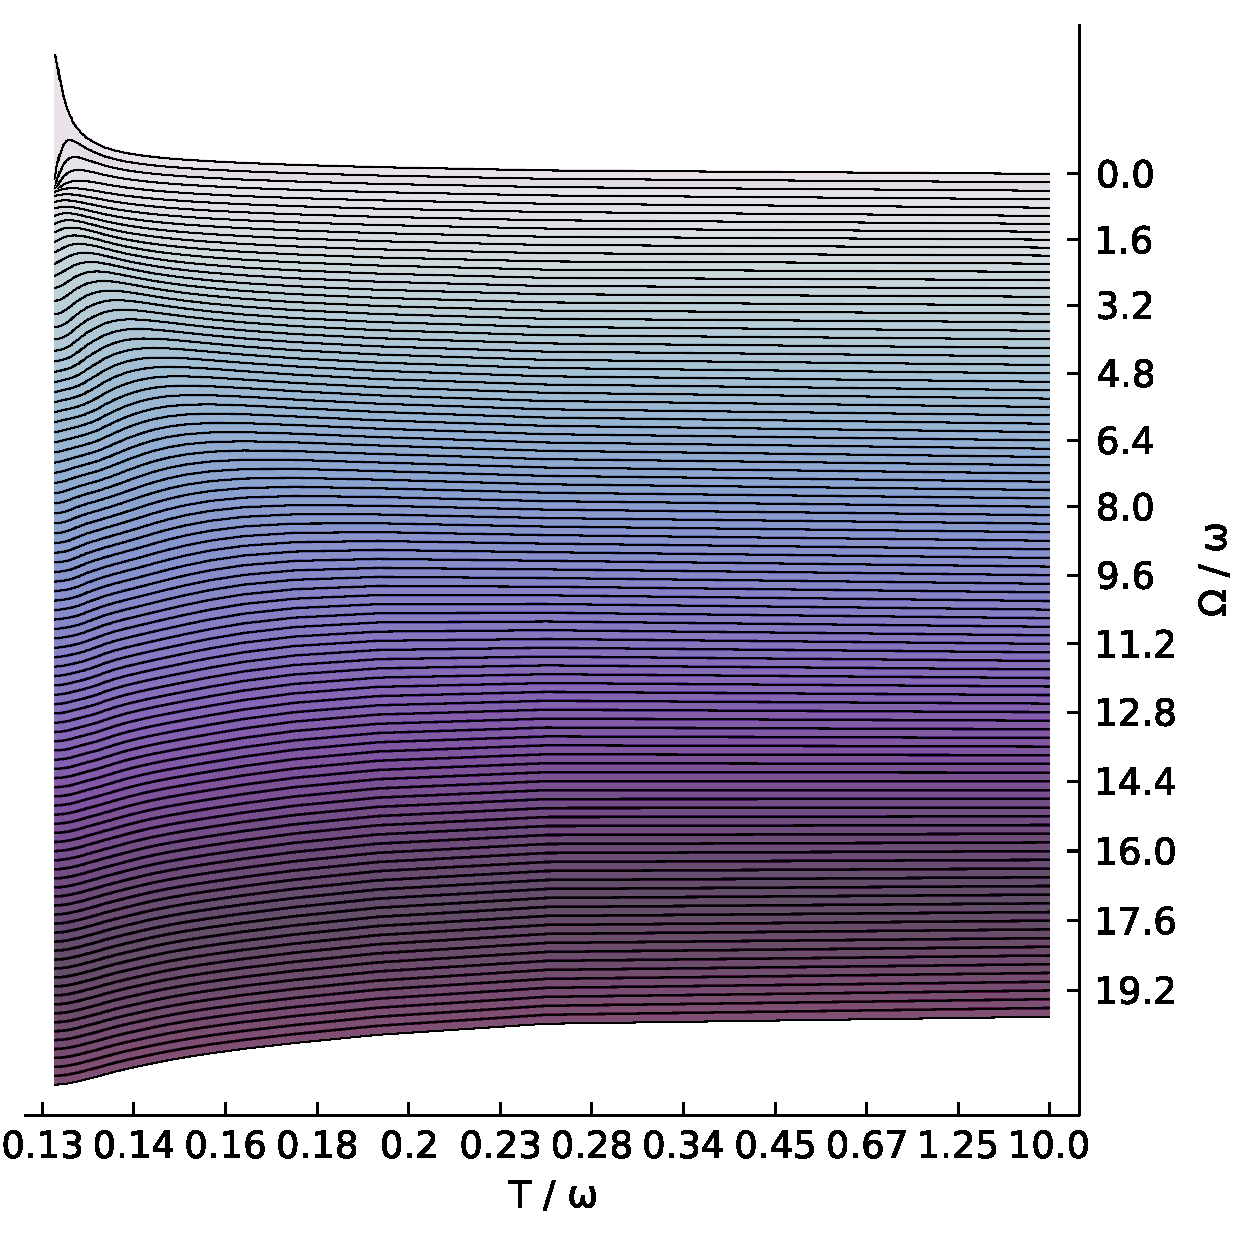
\includegraphics[width=.9\textwidth]{chapters/frohlich/figures/conductivity_plot_freq_real_3.pdf}
\end{subfigure}%
\begin{subfigure}[t]{0.01\textwidth}
    \vspace*{-7.5cm}\textbf{b}
  \end{subfigure}
\begin{subfigure}[b]{.58\textwidth}
\centering
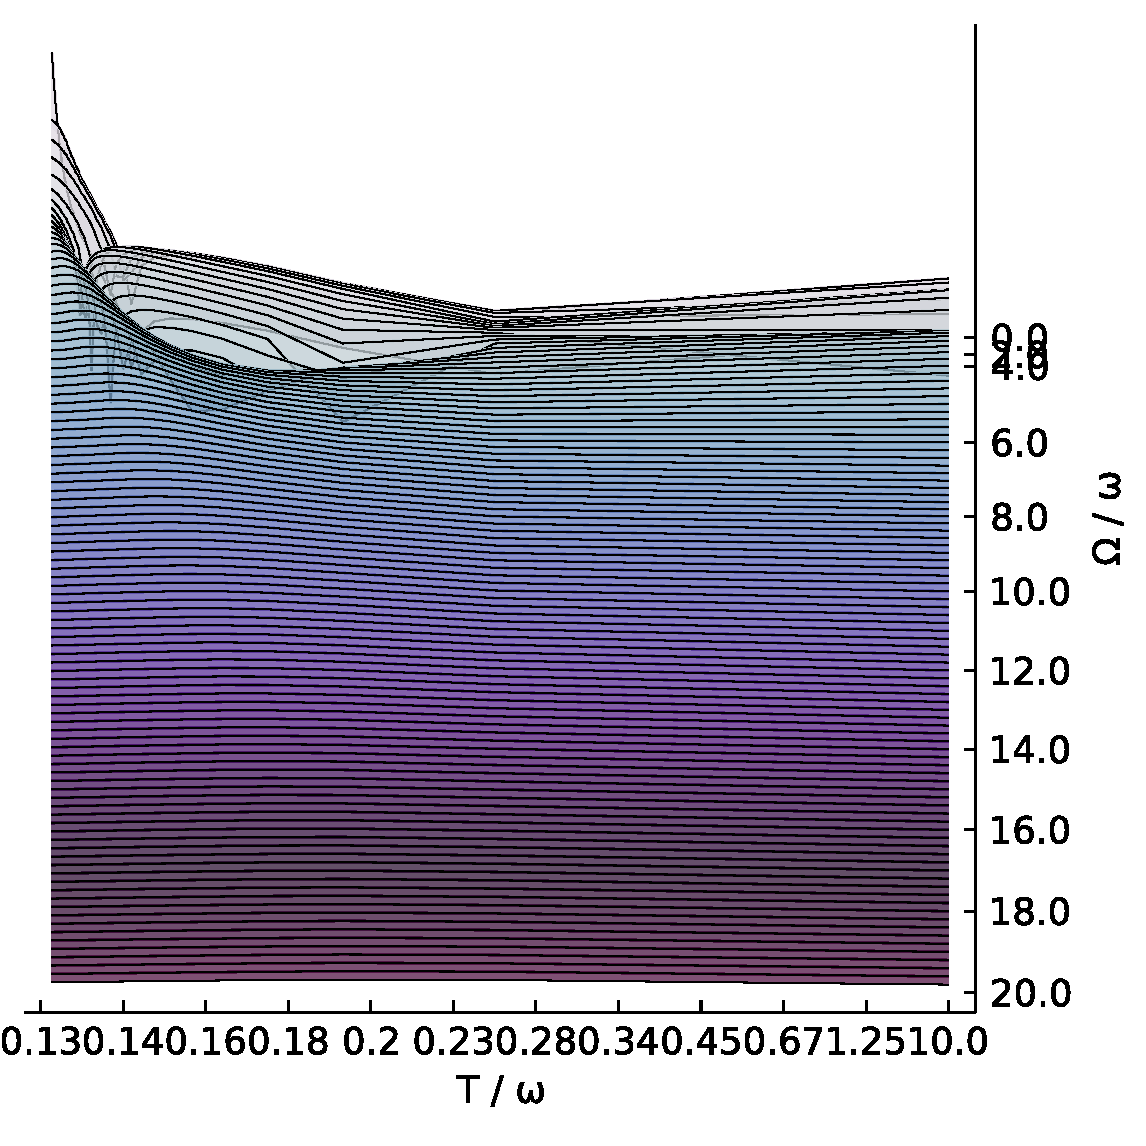
\includegraphics[width=.9\textwidth]{chapters/frohlich/figures/conductivity_plot_freq_imag_3.pdf}
\end{subfigure}%
}\\
\makebox[\linewidth][c]{%
\begin{subfigure}[t]{0.01\textwidth}
    \vspace*{-7.5cm}\textbf{c}
  \end{subfigure}%
\begin{subfigure}[b]{.58\textwidth}
\centering
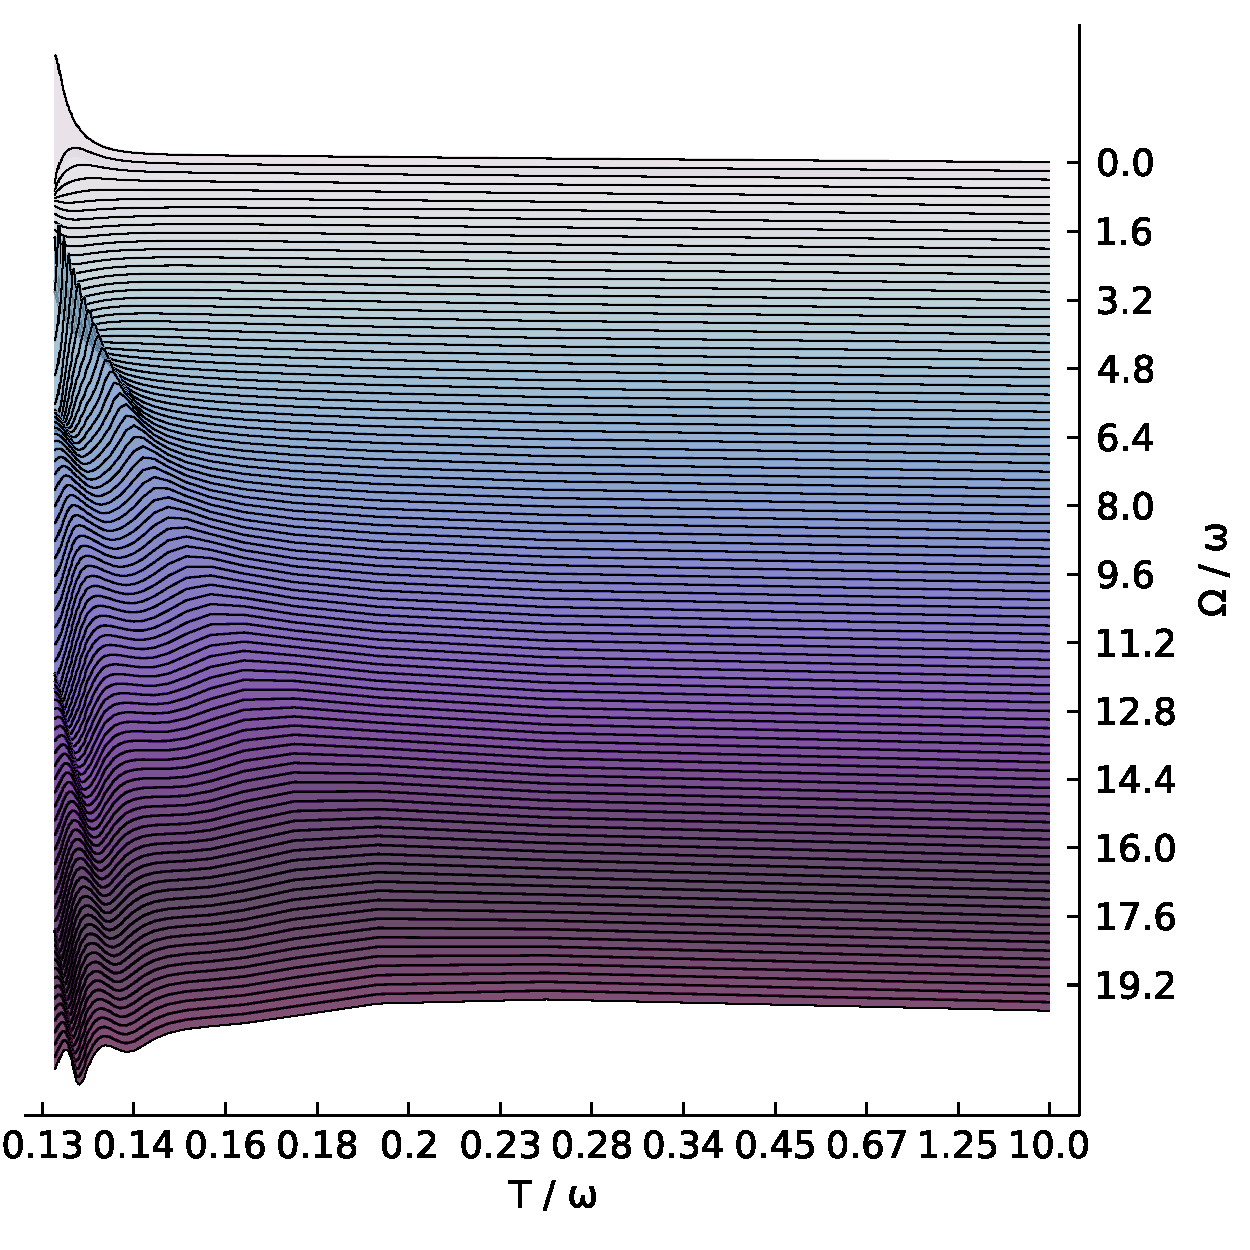
\includegraphics[width=.9\textwidth]{chapters/frohlich/figures/conductivity_plot_freq_real_6.pdf}
\end{subfigure}%
\begin{subfigure}[t]{0.01\textwidth}
    \vspace*{-7.5cm}\textbf{d}
  \end{subfigure}%
\begin{subfigure}[b]{.58\textwidth}
\centering
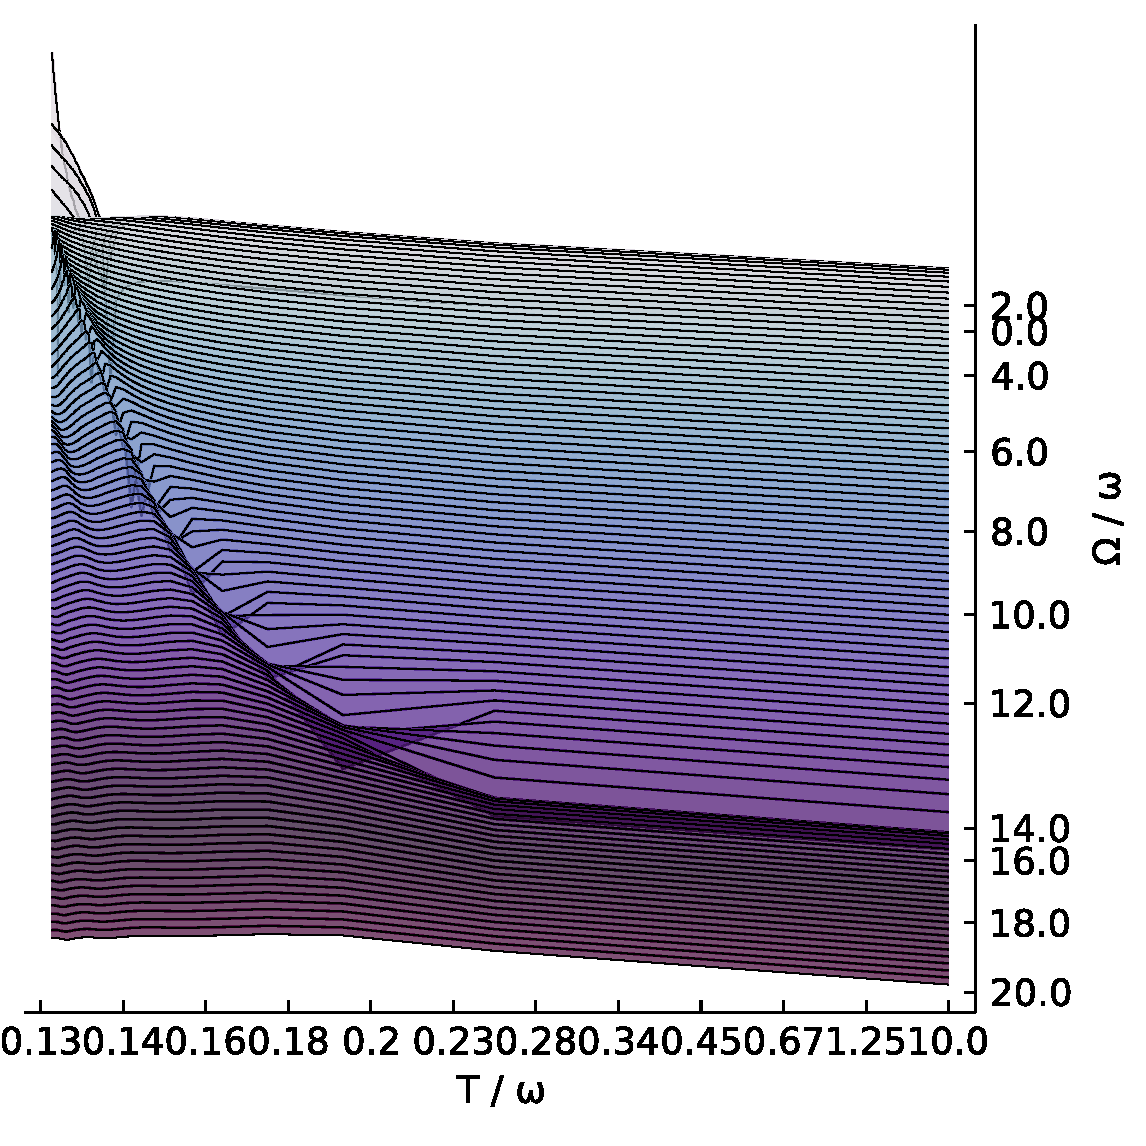
\includegraphics[width=.9\textwidth]{chapters/frohlich/figures/conductivity_plot_freq_imag_6.pdf}
\end{subfigure}%
}
\makebox[\linewidth][c]{%
\begin{subfigure}[t]{0.01\textwidth}
    \vspace*{-7.5cm}\textbf{e}
  \end{subfigure}%
\begin{subfigure}[b]{.58\textwidth}
\centering
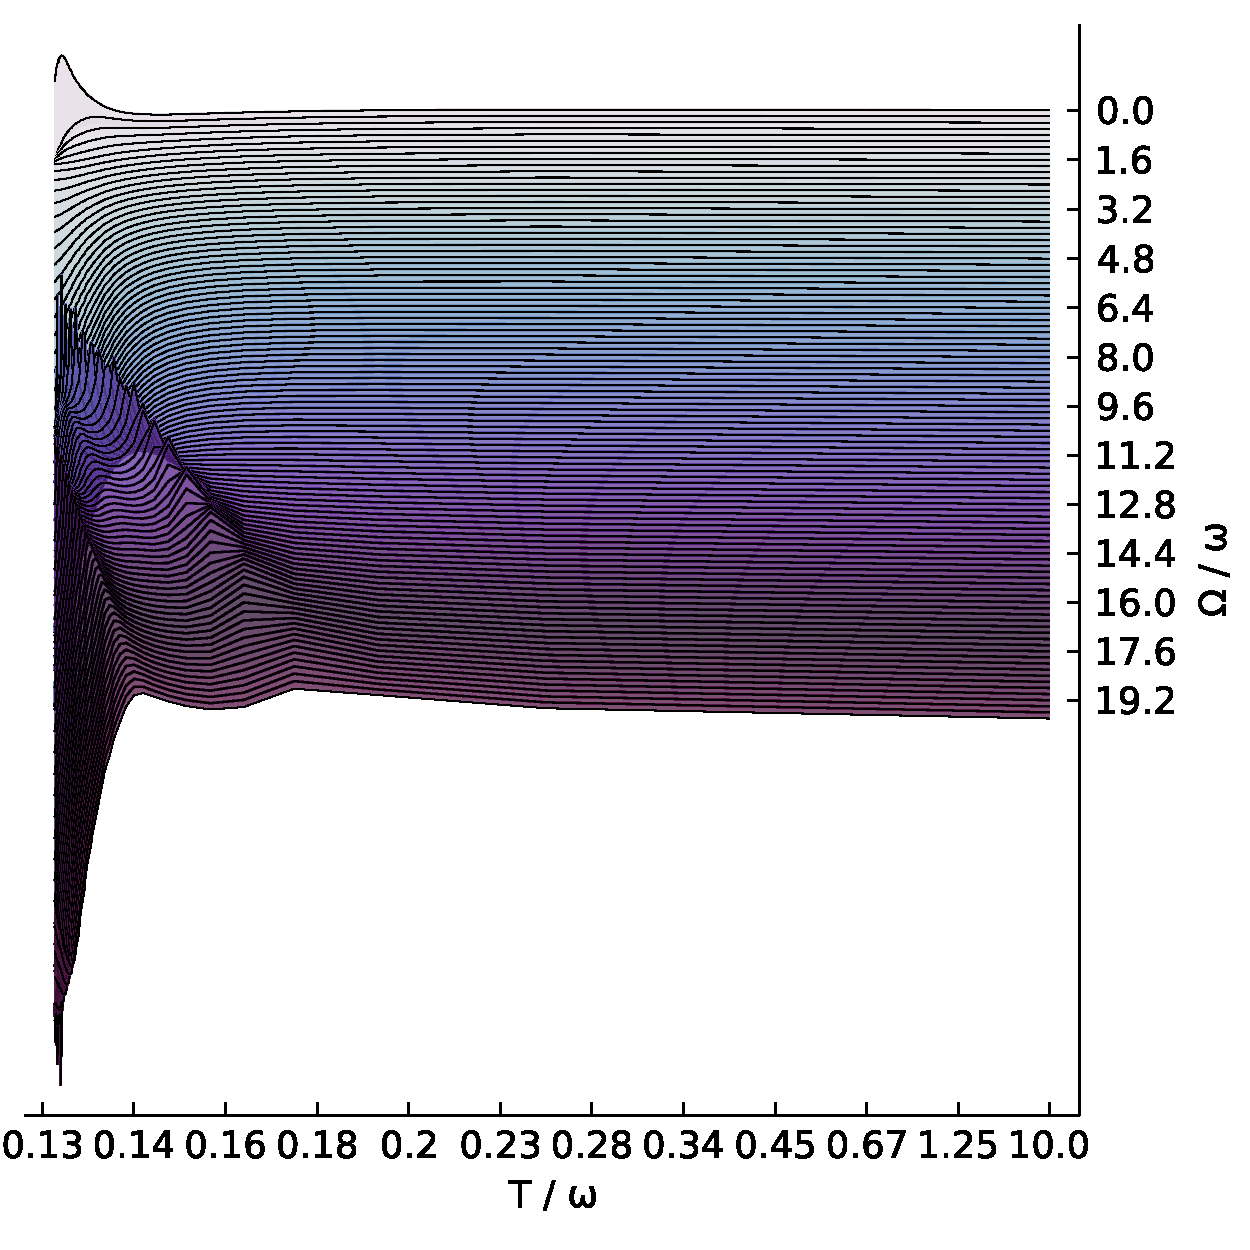
\includegraphics[width=.9\textwidth]{chapters/frohlich/figures/conductivity_plot_freq_real_9.pdf}
\end{subfigure}%
\begin{subfigure}[t]{0.01\textwidth}
    \vspace*{-7.5cm}\textbf{f}
  \end{subfigure}%
\begin{subfigure}[b]{.58\textwidth}
\centering
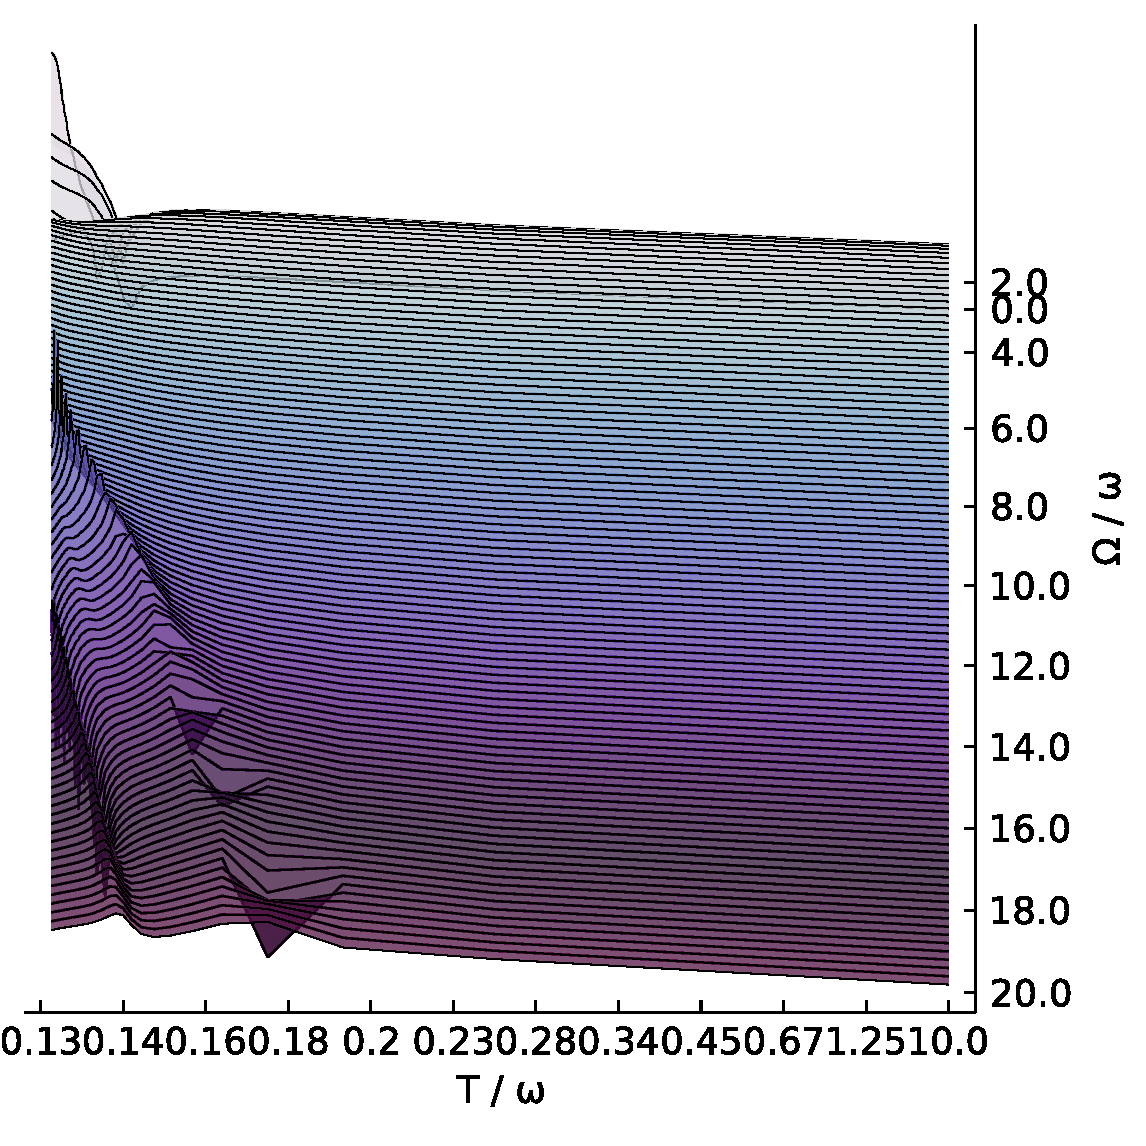
\includegraphics[width=.9\textwidth]{chapters/frohlich/figures/conductivity_plot_freq_imag_9.pdf}
\end{subfigure}%
}
\caption{The same ridgeline plots as in Figure 5 but with the y- and x-axes swapped. }
\end{figure}

\subsection{Multiple phonon branches}

\begin{table}
\begin{center}
\begin{tabular}{||c|c|c|c||} 
\hline\hline
Phonon Frequencies (THz) & IR Activity & $\epsilon^{\text{ionic}}_j$ & $\alpha_j$ \\
\hline\hline
4.017 & 0.082 & 0.300 & 0.034 \\
\hline
3.888 & 0.006 & 0.025 & 0.003 \\
\hline
3.531 & 0.054 & 0.254 & 0.031 \\ 
\hline
2.755 & 0.021 & 0.166 & 0.023 \\
\hline
2.438 & 0.232 & 2.308 & 0.336 \\
\hline
2.249 & 0.262 & 3.071 & 0.465 \\
\hline
2.080 & 0.234 & 3.203 & 0.505 \\
\hline
2.034 & 0.062 & 0.893 & 0.142 \\
\hline
1.567 & 0.037 & 0.886 & 0.161 \\
\hline
1.019 & 0.013 & 0.721 & 0.162 \\
\hline
1.002 & 0.007 & 0.402 & 0.091 \\
\hline
0.997 & 0.010 & 0.618 & 0.141 \\
\hline
0.920 & 0.011 & 0.767 & 0.182 \\
\hline
0.801 & 0.002 & 0.156 & 0.040 \\
\hline
0.574 & 0.007 & 1.163 & 0.349 \\
\hline\hline
\end{tabular} \label{table:mapidata}
\caption{Infrared activity, ionic dielectric contribution and decomposed Fr\"ohlich alpha values associated with each of the phonon modes in MAPbI3 taken from Ref~\cite{brivio_lattice_2015}. The effective Fr\"ohlich alpha $\alpha_{\text{eff}} = \sum_j \alpha_j$ is found to be $2.66$ for MAPbI3.}
\end{center}
\end{table}

I have produced a Julia Pluto.jl notebook that uses the multiple phonon theory to evaluate the decomposed Fr\"ohlich $\alpha_j$ components associated with $15$ modes of Methylammonium lead iodide (MAPbI$_3$). The frequencies and infrared activities associated with these modes are listed in Table 1. The decomposed $\alpha_j$ parameters and phonon frequencies $\omega_j$ are then inserted into the variational principle for multiple phonons to obtain a $v$ and $w$ parameter that provide the lowest upper-bound to the exact free energy of the multi-modal polaron system. The two effective phonon frequencies schemes, labelled scheme A and B in~\cite{hellwarth_mobility_1999} (c.f. section 3.6.5), evaluate the Fr\"ohlich alpha for MAPbI$_3$ to be $\alpha = 2.52$ (towards zero temperature the A scheme gives a slightly different value of $2.44$). In comparison, including the ionic contributions of each MAPbI$_3$ phonon modes explicitly produced the decomposed Fr\"ohlich alpha $\alpha_j$ shown in Table 1. From these, I obtain an effective alpha for MAPbI$_3$ of $\alpha_{\text{eff}} = 2.66$ which is only slightly larger than the value predicted by the effective mode A and B schemes. The free energy approximated by the multiple phonon theory is shown in comparison the Hellwarth and Biaggio effective mode theory in Figure \ref{fig:multitheory}a. The two Hellwarth schemes agree for almost all temperatures except for a small deviation towards zero temperature where the A scheme gives a slightly lower value. The multiple phonon theory clearly gives a lower estimate to the free energy of the polaron compared to the Hellwarth theory for all temperatures above roughly $100$K but gives a higher value at lower temperatures and at zero temperature. Figure \ref{fig:multitheory}b shows a comparison between the multiple phonon variational $v$ and $w$ parameters compared to the effective variational parameters from the Hellwarth and Biaggio effective mode theory. The two agree at zero temperature, but the multiple phonon theory predicts larger polaron frequencies at higher temperatures and a smaller different in $v$ and $w$, $v - w$, at all temperatures. 

\begin{figure}[t]
\vspace*{-1.5cm}\makebox[\linewidth][c]{%
\begin{subfigure}[b]{.6\textwidth}
\centering
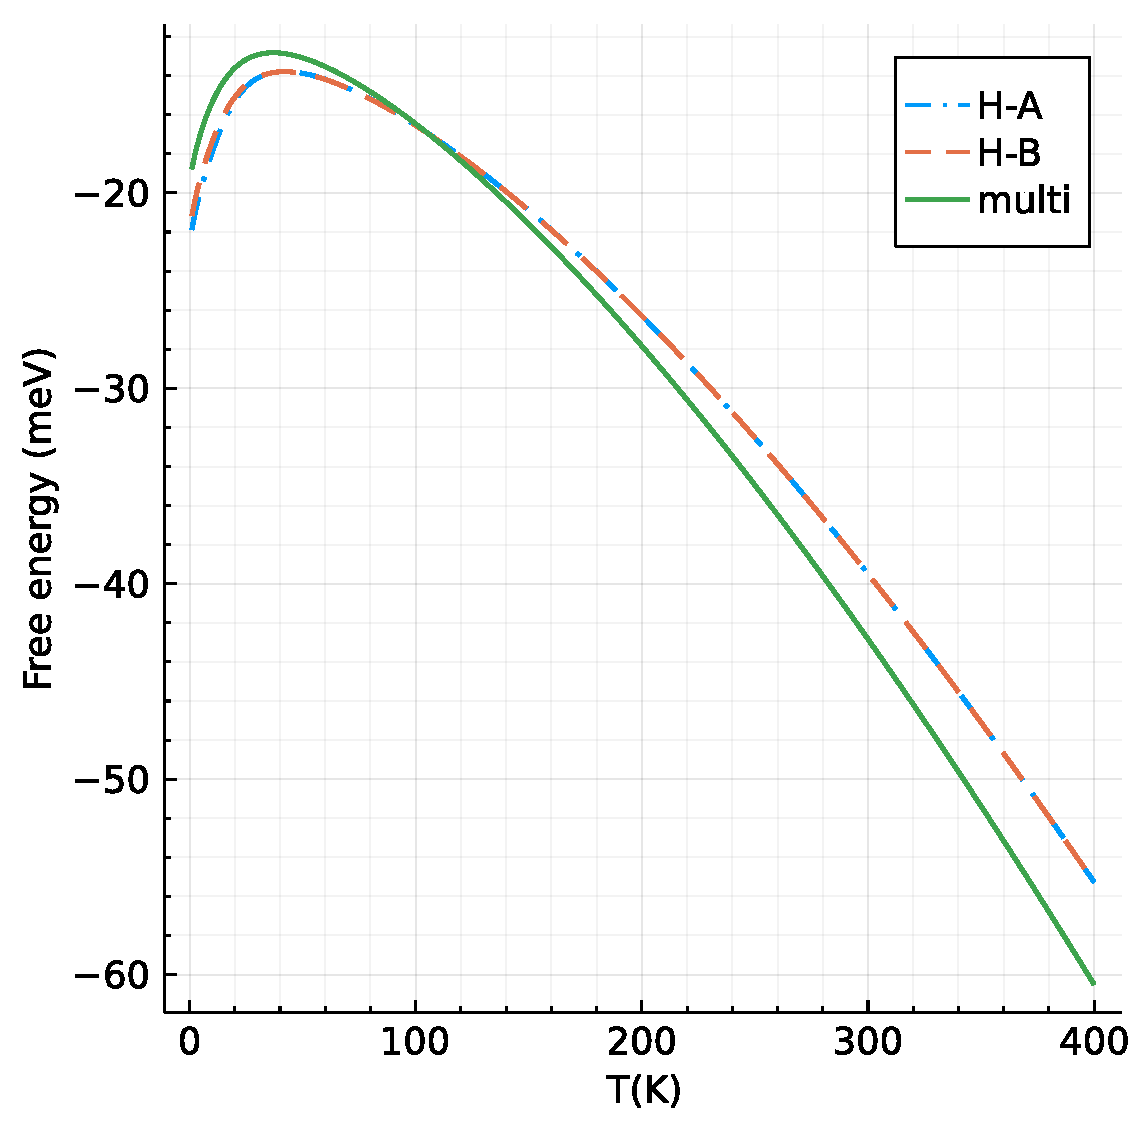
\includegraphics[width=.9\textwidth]{chapters/frohlich/figures/free_energy_temp.pdf}
\end{subfigure}%
\begin{subfigure}[b]{.6\textwidth}
\centering
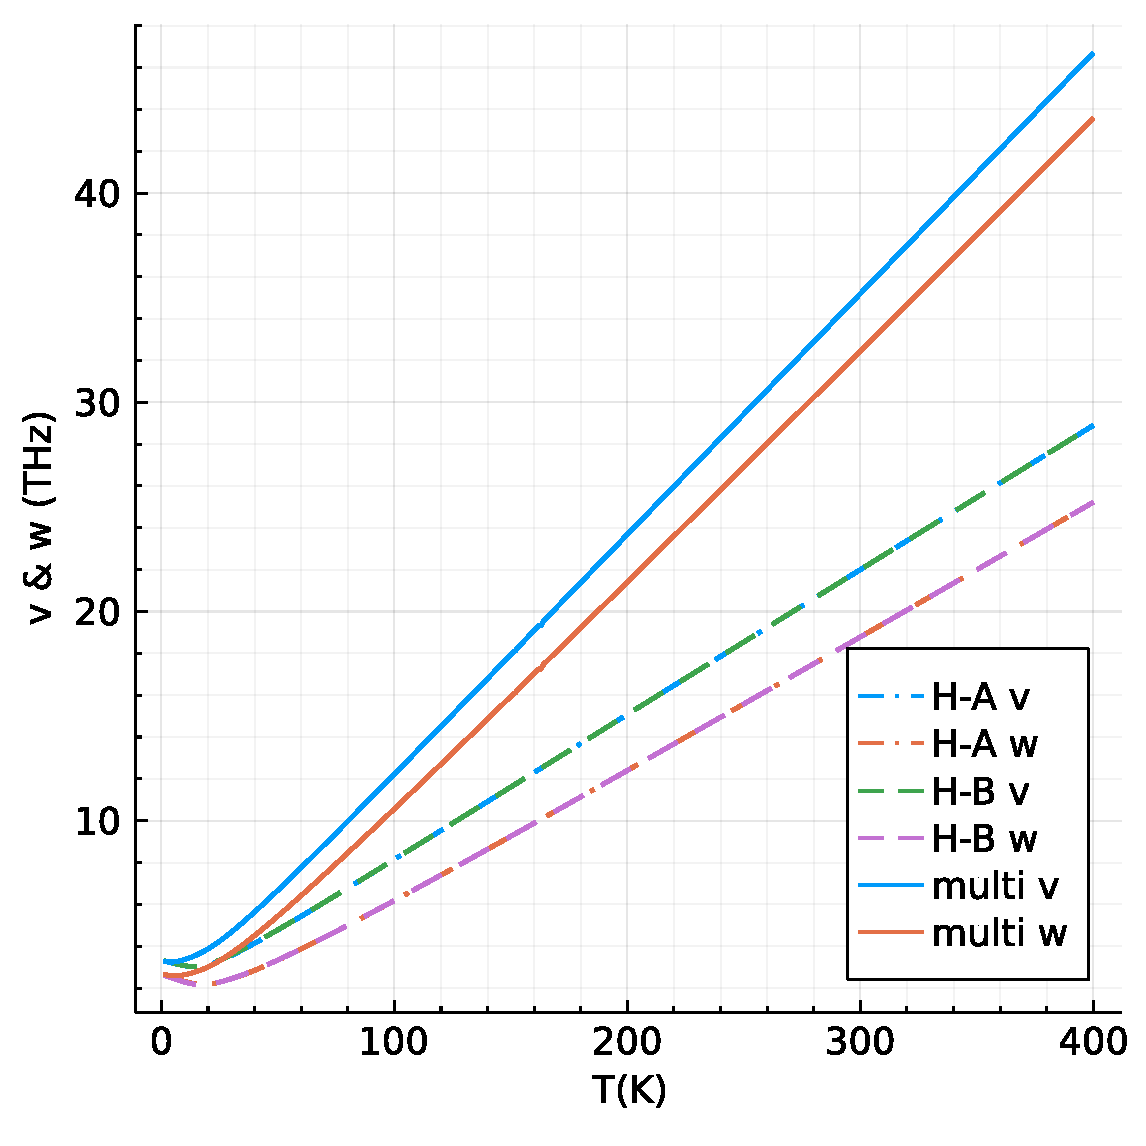
\includegraphics[width=.9\textwidth]{chapters/frohlich/figures/vw_temp.pdf}
\end{subfigure}%
}
\caption{(left): The free energy of the Hellwarth and Biaggio effective mode A \& B schemes and for the multiple phonon model between $1$K and $400$K. The two Hellwarth schemes agree almost exactly except for a small deviation at low temperatures. The multiple phonon model gives a lower free energy estimate for temperatures above $100$K. (right): The variational parameters $v$ \& $w$ from the Hellwarth and Biaggio effective mode A \& B schemes and the multiple phonon model. The effective mode schemes agree whereas the multiple phonon model gives values larger than the Hellwarth schemes but approaches their values towards zero temperature.}
\label{fig:multitheory}
\end{figure}

Figures \ref{fig:multicontour} (contour plots) and \ref{fig:multiridge} (ridge-line plots) compare the complex conductivity obtained from the multiple phonon model (left column) to the complex conductivity obtained from the Hellwarth and Biaggio B scheme (right column). The top rows show the real part of the conductivity (i.e. the ac mobility), the middle rows show the imaginary part and the bottom rows show the absolute value. I chose the B scheme over the A scheme because the B scheme involves matching an effective frequency to the full extent of \=Osaka's finite temperature variational principle, so is arguably more accurate. On the other hand, the A scheme produces a temperature-dependent Fr\"ohlich alpha parameter and effective phonon frequency. This is unlike the original Fr\"ohlich alpha and phonon frequency which are independent of temperature. Nonetheless, the two schemes do produce near-identical results for most temperature anyway, except for a slight deviation at very low temperatures. So, a lot of the comparison with the B scheme will be comparable to that of the A scheme too. 

Both the multiple phonon theory and the Hellwarth and Biaggio effective mode theory have similar dc mobilities and high temperature complex conductivities. Likewise, they both possess a broad peak starting around a frequency of $2.03$ THz, which is the effective phonon frequency derived from the B scheme. (At zero temperature, the A scheme gives an effective phonon frequency of $2.17$ THz). The start of the main peak then shifts up in frequency as the temperature increases whilst primarily broadening and flattening. The theories differ in their frequency dependence. Whilst both possess the same main peak starting around $2$ THz, the multiple phonon theory possesses extra peaks below $2$ THz, particular two fairly sharp peaks starting around $0.50$ THz and $1.00$ THz. All of these extra details are washed-out at higher temperatures to leave one main broad peak that has a maximum located at a slightly lower frequency compared to Hellwarth's and Biaggio's theory.

\begin{figure}
\vspace*{-1.5cm}\makebox[\linewidth][c]{%
\begin{subfigure}[t]{0.01\textwidth}
    \vspace*{-8.1cm}\hspace*{9.3cm}\textbf{\underline{Real}}
    \vspace*{-7.5cm}\textbf{a}
  \end{subfigure}%
\begin{subfigure}[b]{.6\textwidth}
\centering
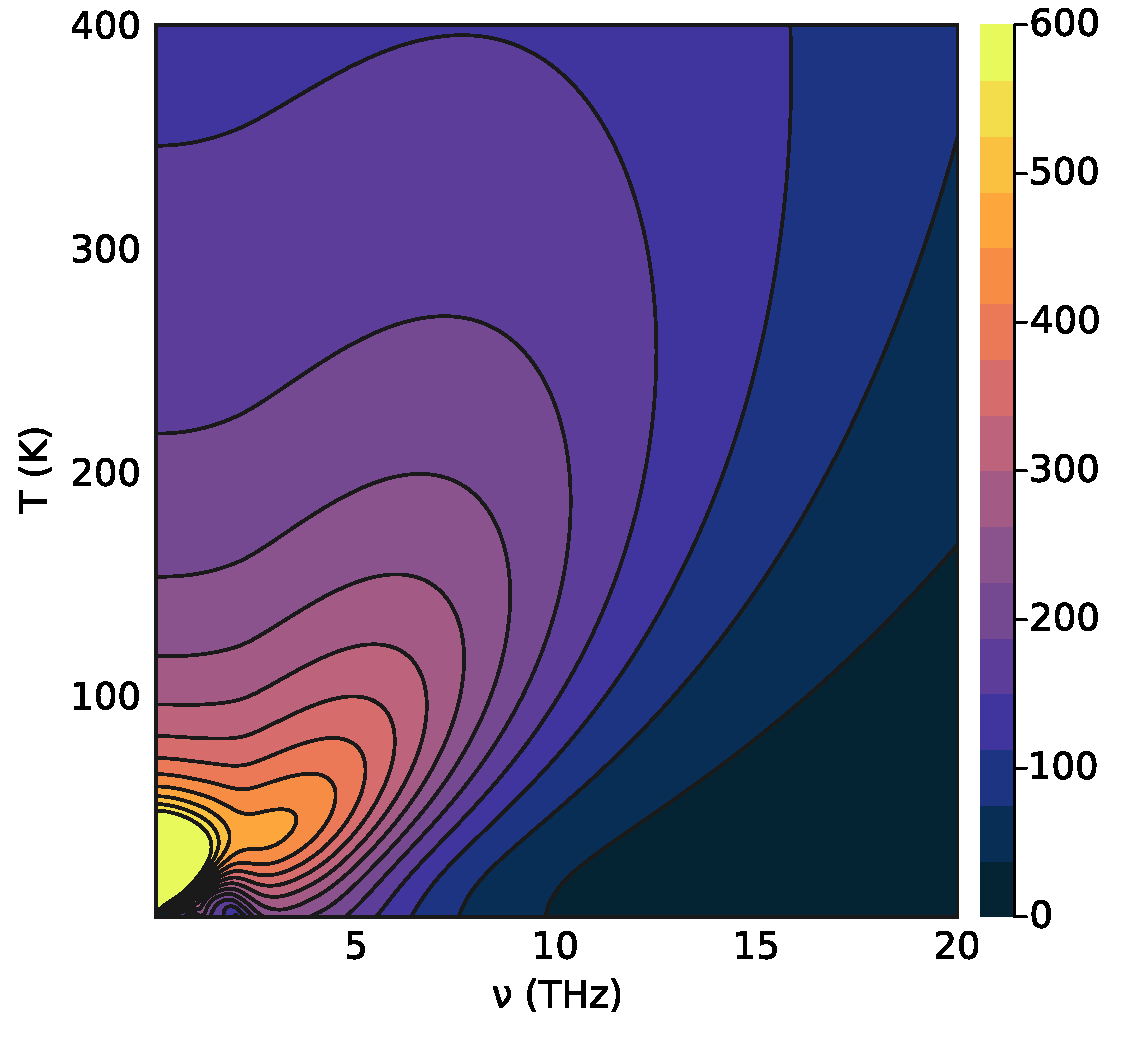
\includegraphics[width=.9\textwidth]{chapters/frohlich/figures/multi_contour_real.pdf}
\end{subfigure}%
\begin{subfigure}[t]{0.01\textwidth}
    \vspace*{-7.5cm}\textbf{b}
  \end{subfigure}
\begin{subfigure}[b]{.6\textwidth}
\centering
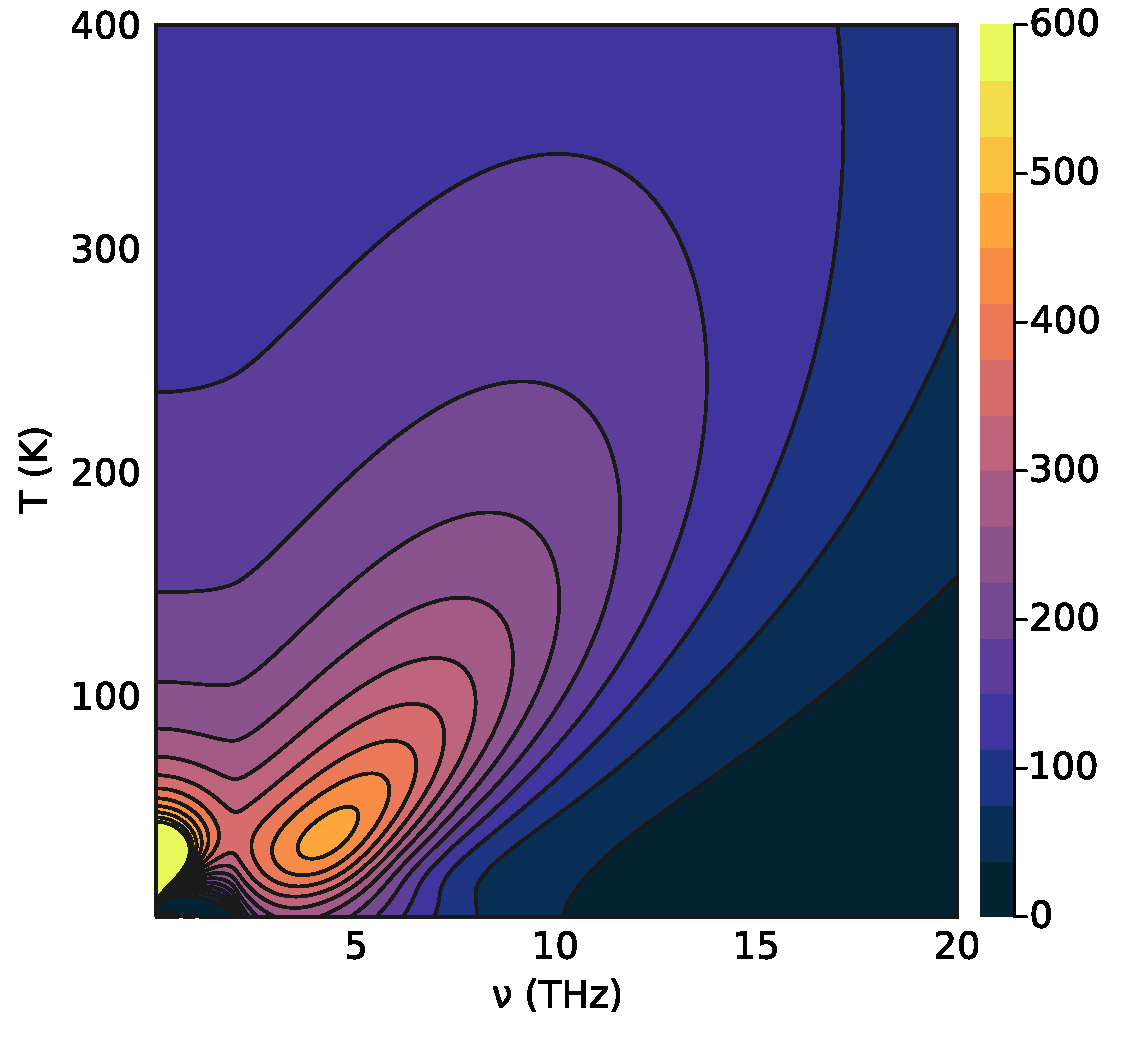
\includegraphics[width=.9\textwidth]{chapters/frohlich/figures/B_contour_real.pdf}
\end{subfigure}%
}\\
\makebox[\linewidth][c]{%
\begin{subfigure}[t]{0.01\textwidth}
    \vspace*{-8.1cm}\hspace*{9.3cm}\textbf{\underline{Imag}}
    \vspace*{-7.5cm}\textbf{c}
  \end{subfigure}%
\begin{subfigure}[b]{.6\textwidth}
\centering
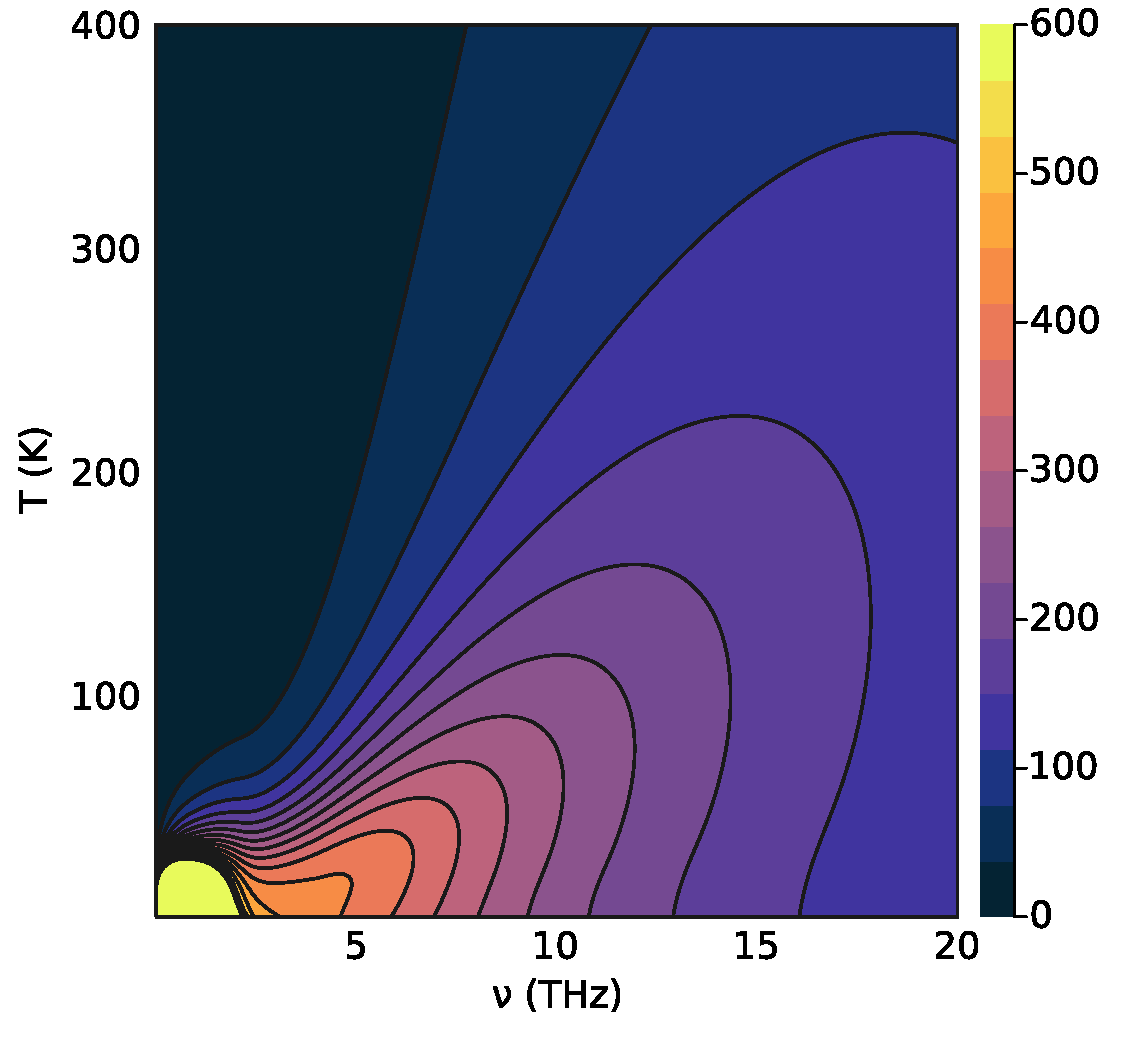
\includegraphics[width=.9\textwidth]{chapters/frohlich/figures/multi_contour_imag.pdf}
\end{subfigure}%
\begin{subfigure}[t]{0.01\textwidth}
    \vspace*{-7.5cm}\textbf{d}
  \end{subfigure}%
\begin{subfigure}[b]{.6\textwidth}
\centering
\includegraphics[width=.9\textwidth]{chapters/frohlich/figures/B_contour_imag.pdf}
\end{subfigure}%
}
\makebox[\linewidth][c]{%
\begin{subfigure}[t]{0.01\textwidth}
    \vspace*{-8.1cm}\hspace*{9.3cm}\textbf{\underline{Abs}}
    \vspace*{-7.5cm}\textbf{e}
  \end{subfigure}%
\begin{subfigure}[b]{.6\textwidth}
\centering
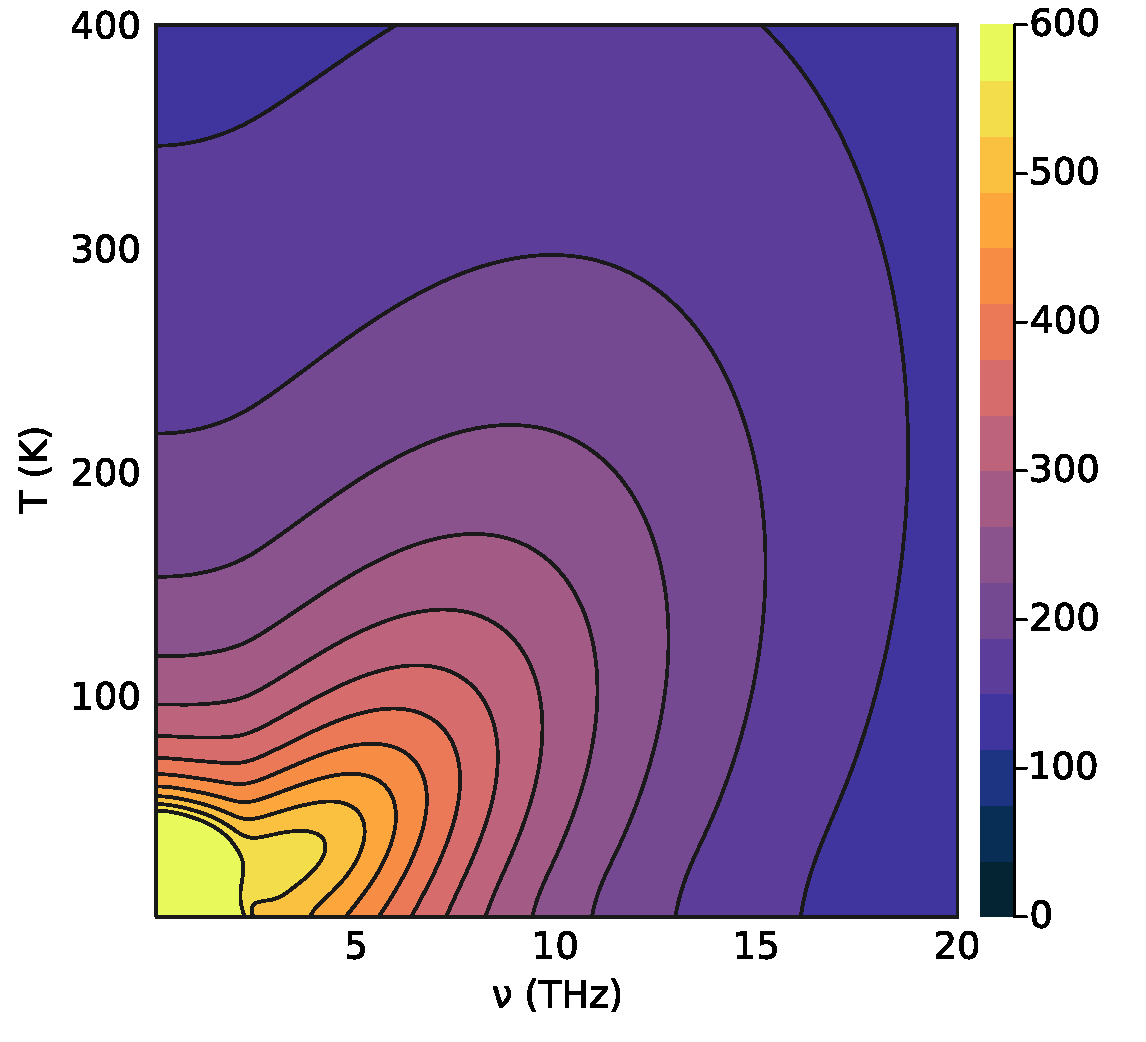
\includegraphics[width=.9\textwidth]{chapters/frohlich/figures/multi_contour_abs.pdf}
\end{subfigure}%
\begin{subfigure}[t]{0.01\textwidth}
    \vspace*{-7.5cm}\textbf{f}
  \end{subfigure}%
\begin{subfigure}[b]{.6\textwidth}
\centering
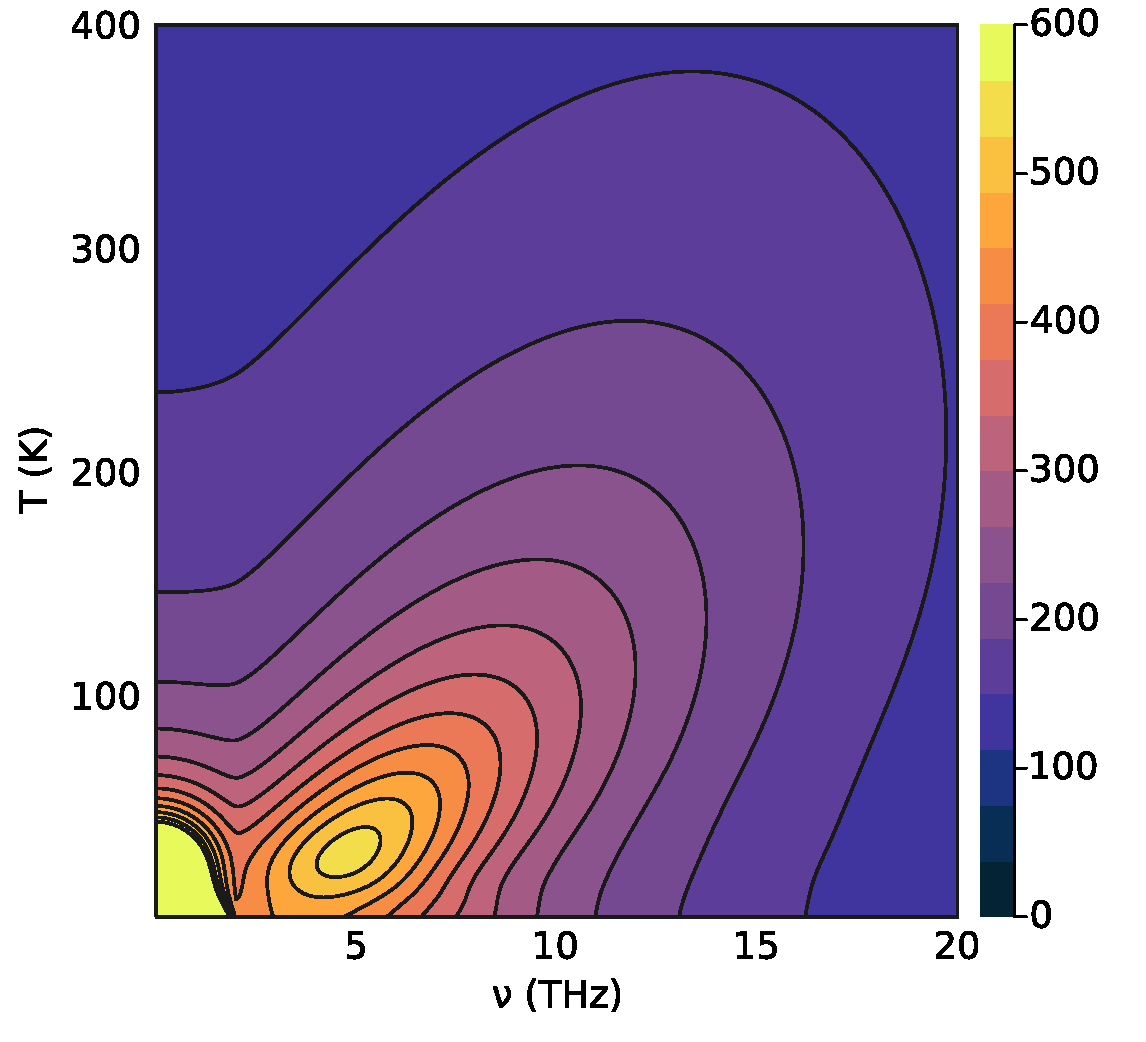
\includegraphics[width=.9\textwidth]{chapters/frohlich/figures/B_contour_abs.pdf}
\end{subfigure}%
}
\caption{Left: Multiple phonon scheme (a) real conductivity, (c) imaginary conductivity, (e) absolute conductivity. Right: Hellwarth `B' scheme: (b) real conductivity, (d) imaginary conductivity, (f) absolute conductivity.}
\label{fig:multicontour}
\end{figure}

\begin{figure}
\vspace*{-1.5cm}\makebox[\linewidth][c]{%
\begin{subfigure}[t]{0.01\textwidth}
    \vspace*{-8.1cm}\hspace*{9cm}\textbf{\underline{Real}}
    \vspace*{-7.5cm}\textbf{a}
  \end{subfigure}%
\begin{subfigure}[b]{.58\textwidth}
\centering
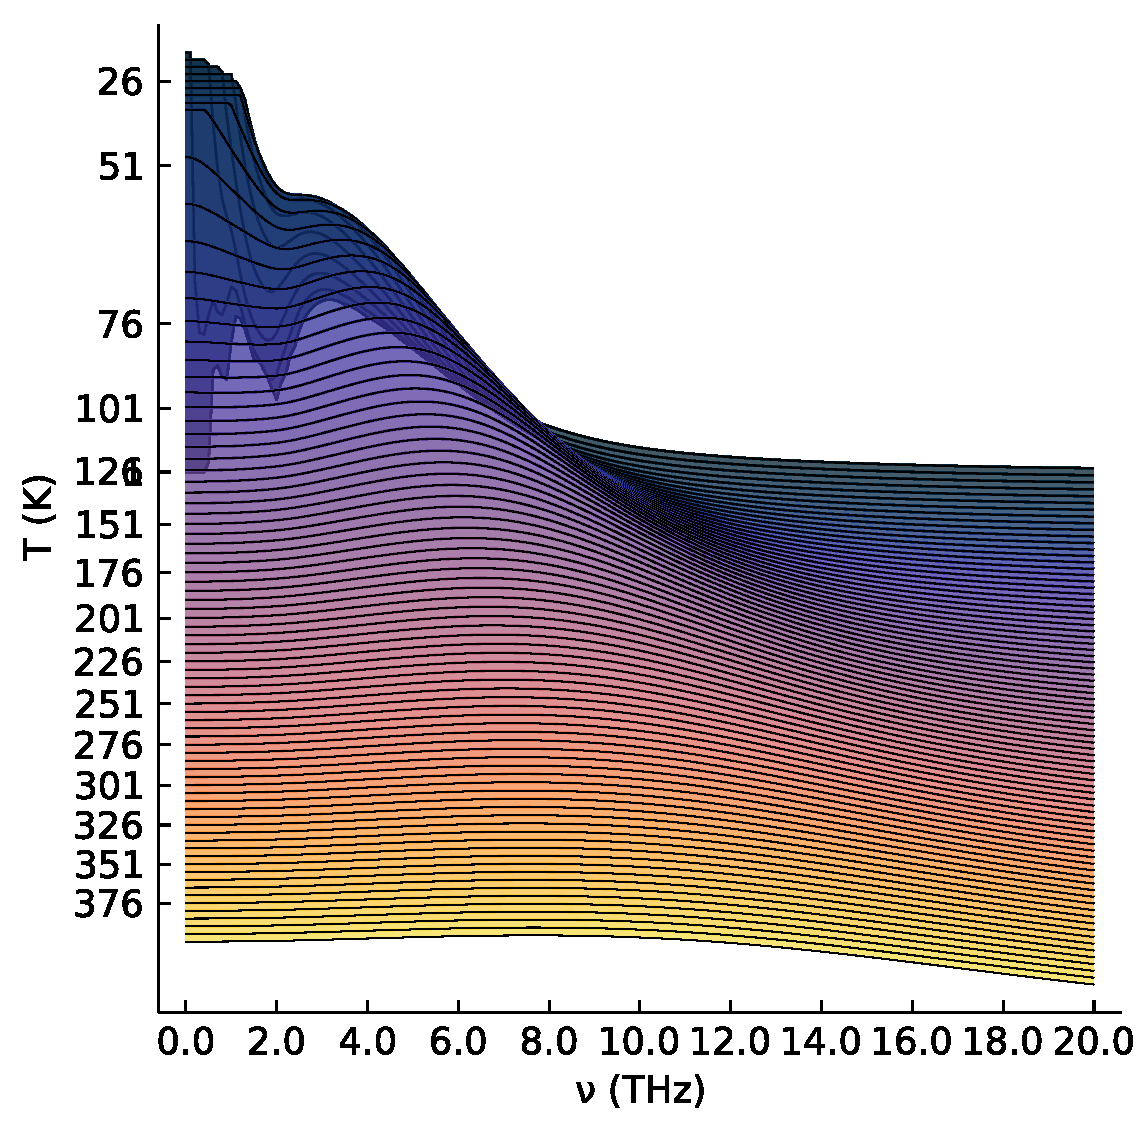
\includegraphics[width=.88\textwidth]{chapters/frohlich/figures/multi_plot_temp_real.pdf}
\end{subfigure}%
\begin{subfigure}[t]{0.01\textwidth}
    \vspace*{-7.5cm}\textbf{b}
  \end{subfigure}
\begin{subfigure}[b]{.58\textwidth}
\centering
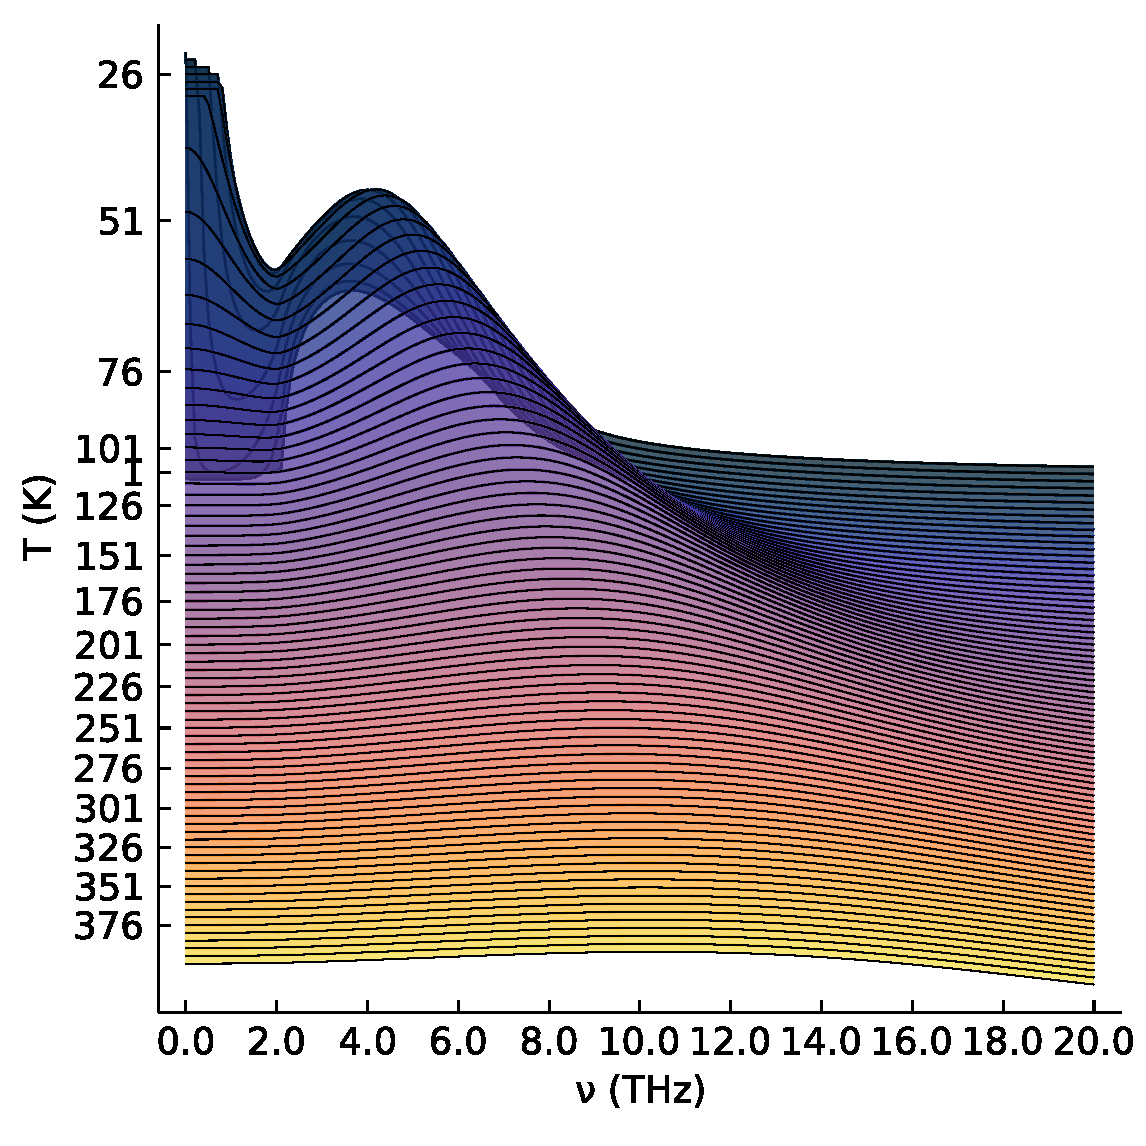
\includegraphics[width=.88\textwidth]{chapters/frohlich/figures/B_plot_temp_real.pdf}
\end{subfigure}%
}\\
\makebox[\linewidth][c]{%
\begin{subfigure}[t]{0.01\textwidth}
    \vspace*{-8.1cm}\hspace*{9cm}\textbf{\underline{Imag}}
    \vspace*{-7.5cm}\textbf{c}
  \end{subfigure}%
\begin{subfigure}[b]{.58\textwidth}
\centering
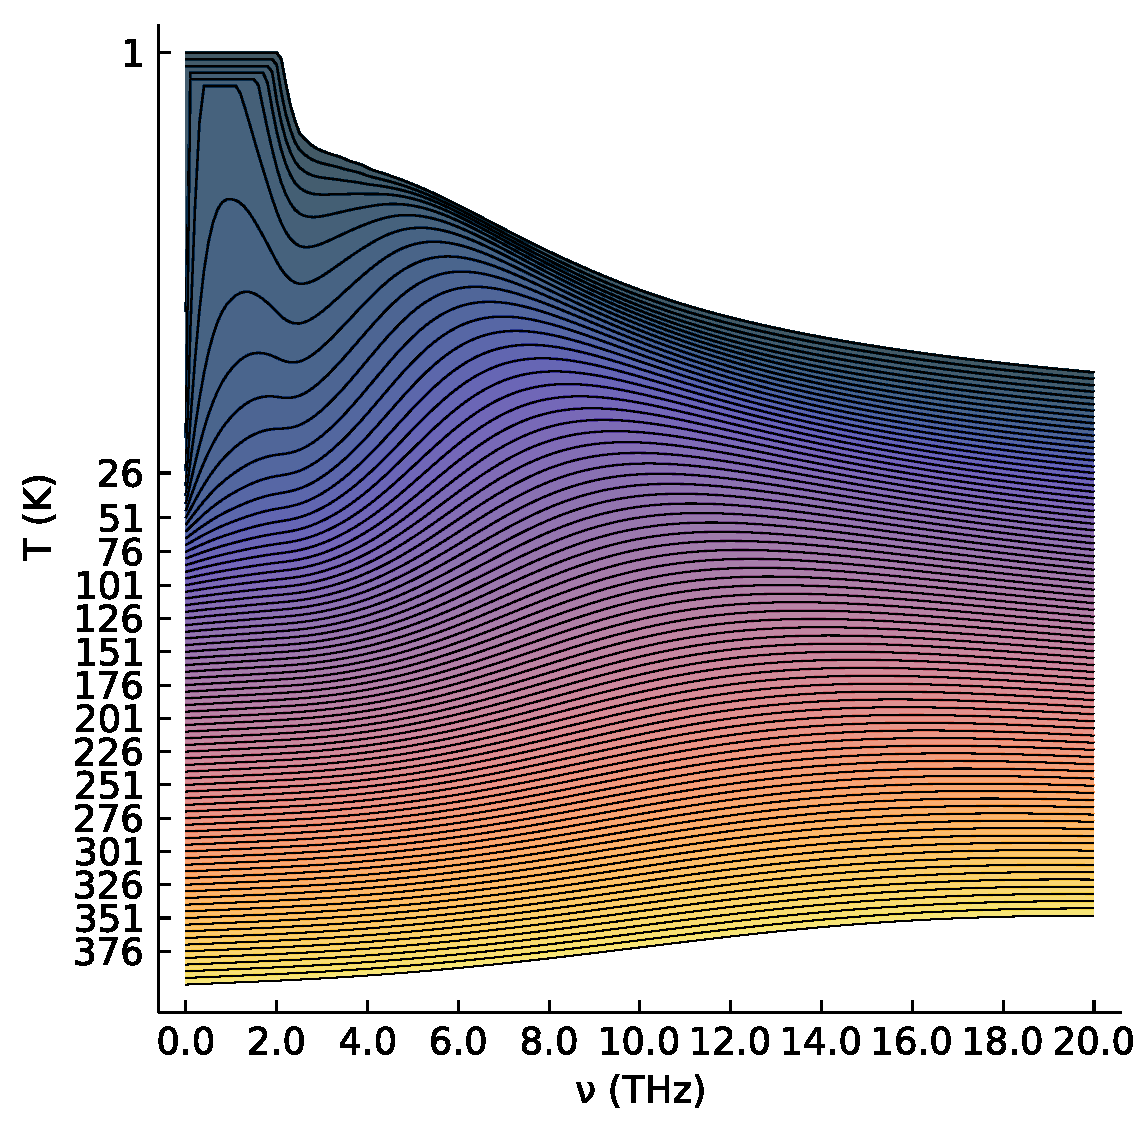
\includegraphics[width=.88\textwidth]{chapters/frohlich/figures/multi_plot_temp_imag.pdf}
\end{subfigure}%
\begin{subfigure}[t]{0.01\textwidth}
    \vspace*{-7.5cm}\textbf{d}
  \end{subfigure}%
\begin{subfigure}[b]{.58\textwidth}
\centering
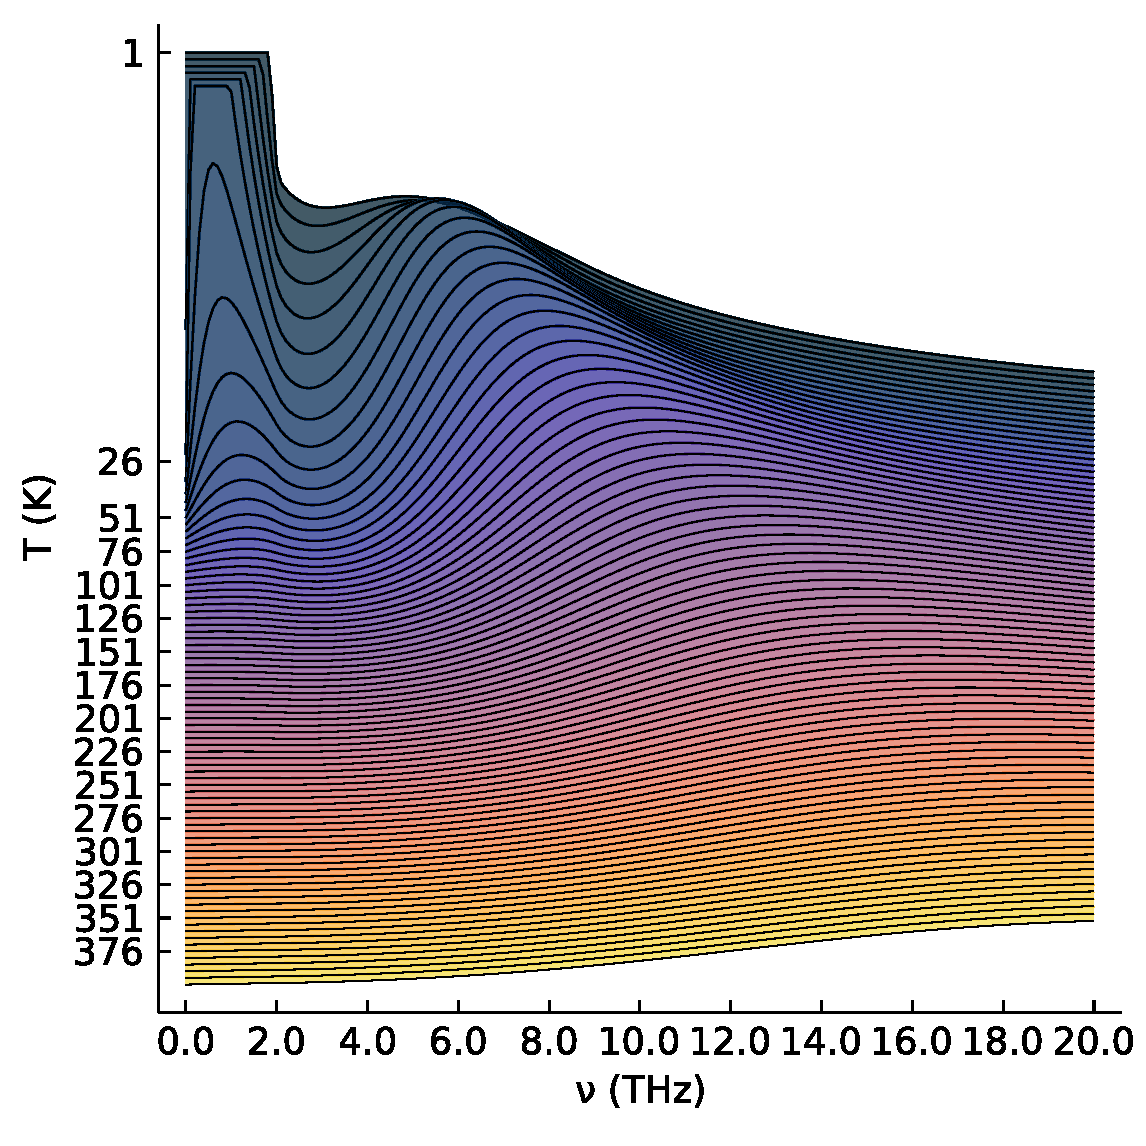
\includegraphics[width=.88\textwidth]{chapters/frohlich/figures/B_plot_temp_imag.pdf}
\end{subfigure}%
}
\makebox[\linewidth][c]{%
\begin{subfigure}[t]{0.01\textwidth}
    \vspace*{-8.1cm}\hspace*{9cm}\textbf{\underline{Abs}}
    \vspace*{-7.5cm}\textbf{e}
  \end{subfigure}%
\begin{subfigure}[b]{.58\textwidth}
\centering
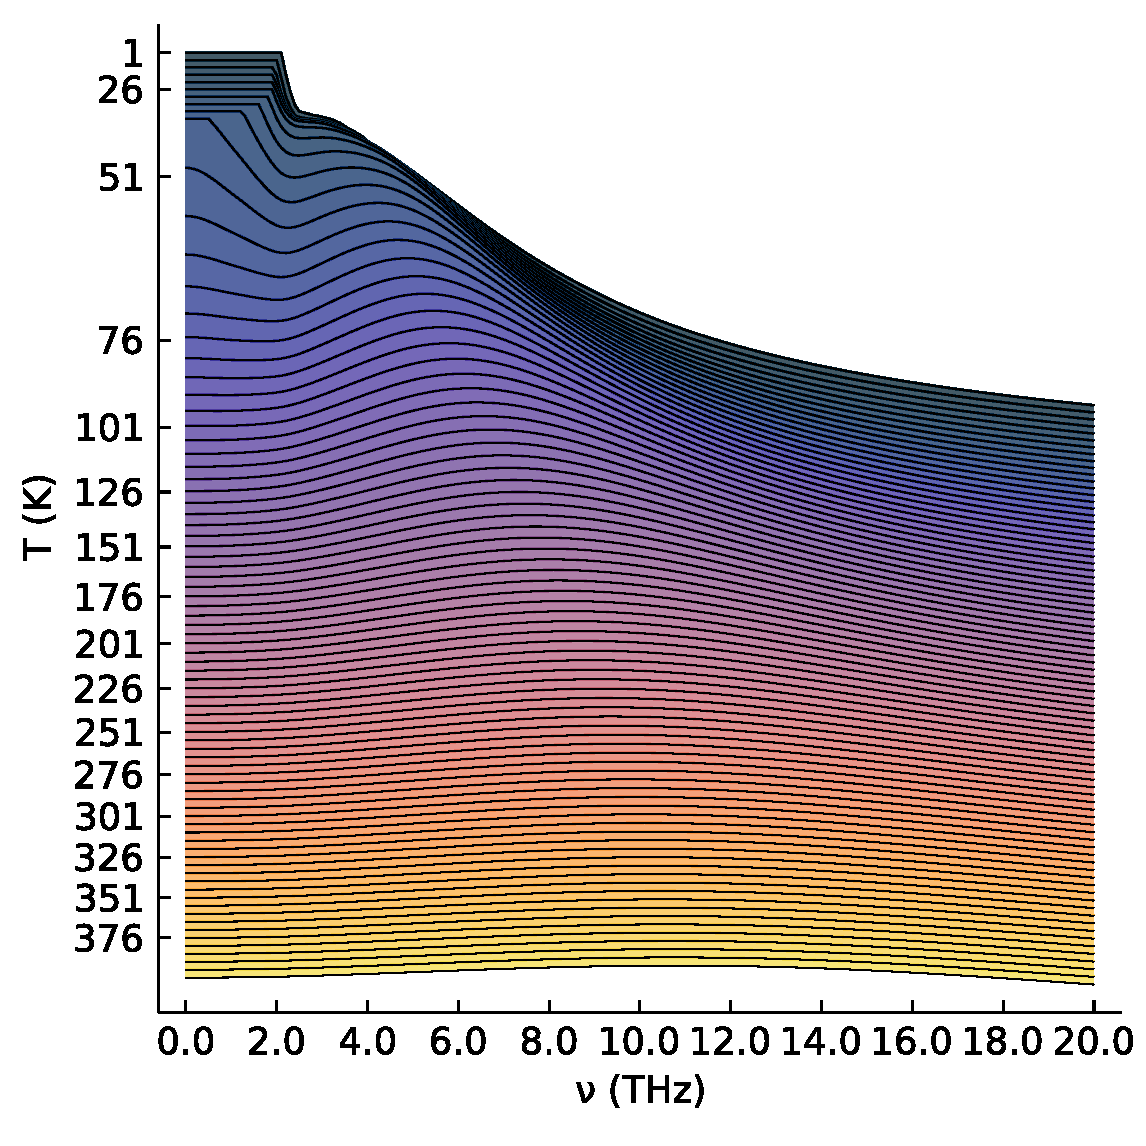
\includegraphics[width=.88\textwidth]{chapters/frohlich/figures/multi_plot_temp_abs.pdf}
\end{subfigure}%
\begin{subfigure}[t]{0.01\textwidth}
    \vspace*{-7.5cm}\textbf{f}
  \end{subfigure}%
\begin{subfigure}[b]{.58\textwidth}
\centering
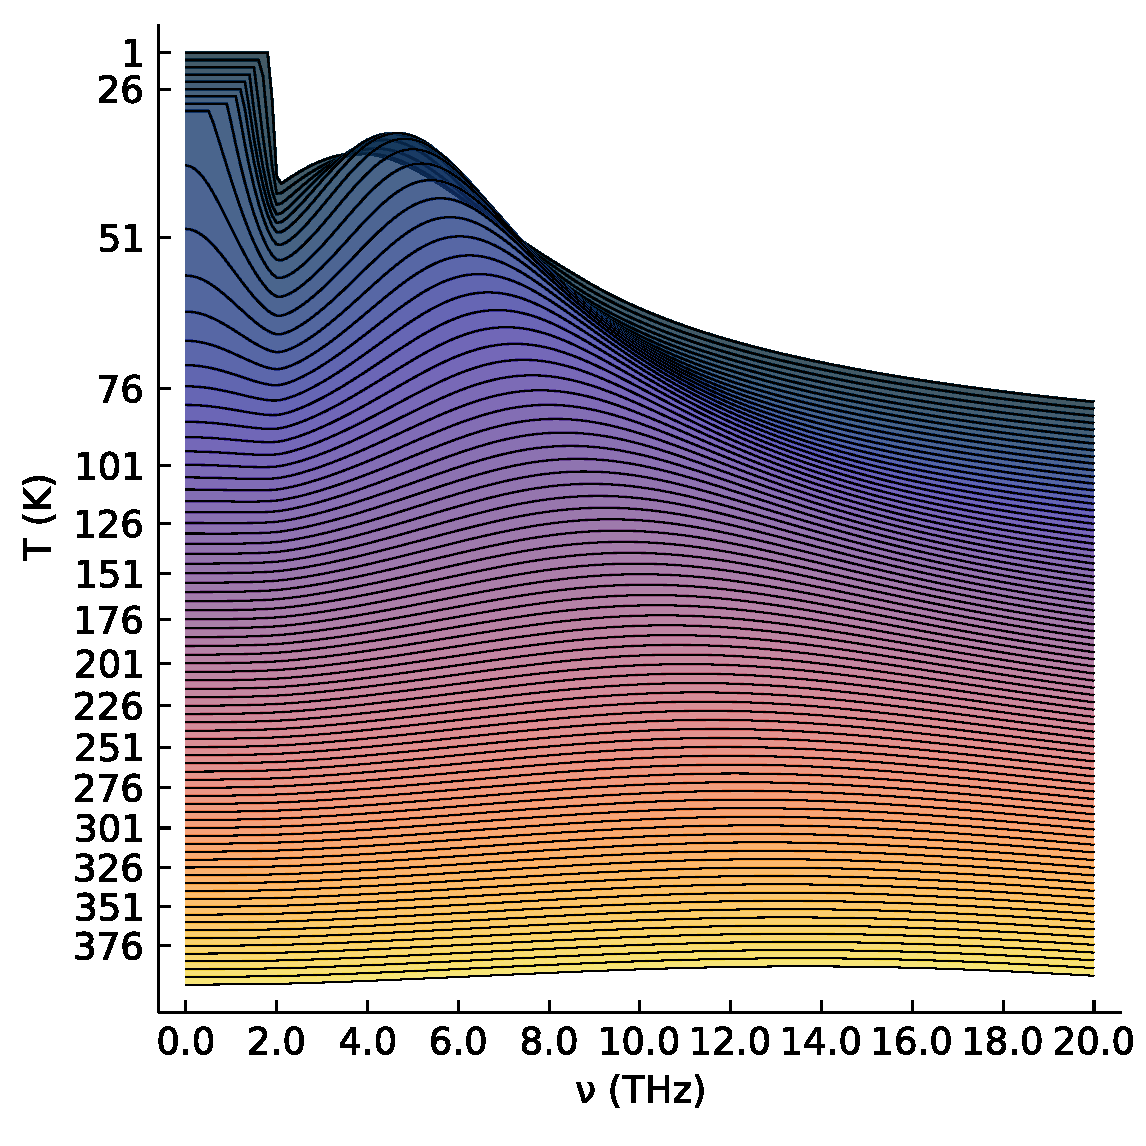
\includegraphics[width=.88\textwidth]{chapters/frohlich/figures/B_plot_temp_abs.pdf}
\end{subfigure}%
}
\caption{Left: Multiple phonon scheme (a) real conductivity, (c) imaginary conductivity, (e) absolute conductivity. Right: Hellwarth `B' scheme: (b) real conductivity, (d) imaginary conductivity, (f) absolute conductivity. At lower temperatures the conductivity has been cut-off at $600$ to enable us to see the main features.}
\label{fig:multiridge}
\end{figure}

\newpage

\begin{figure}
\vspace*{-1.5cm}\makebox[\linewidth][c]{%
\begin{subfigure}[t]{0.01\textwidth}
    \vspace*{-7.5cm}\textbf{a}
  \end{subfigure}%
\begin{subfigure}[b]{.58\textwidth}
\centering
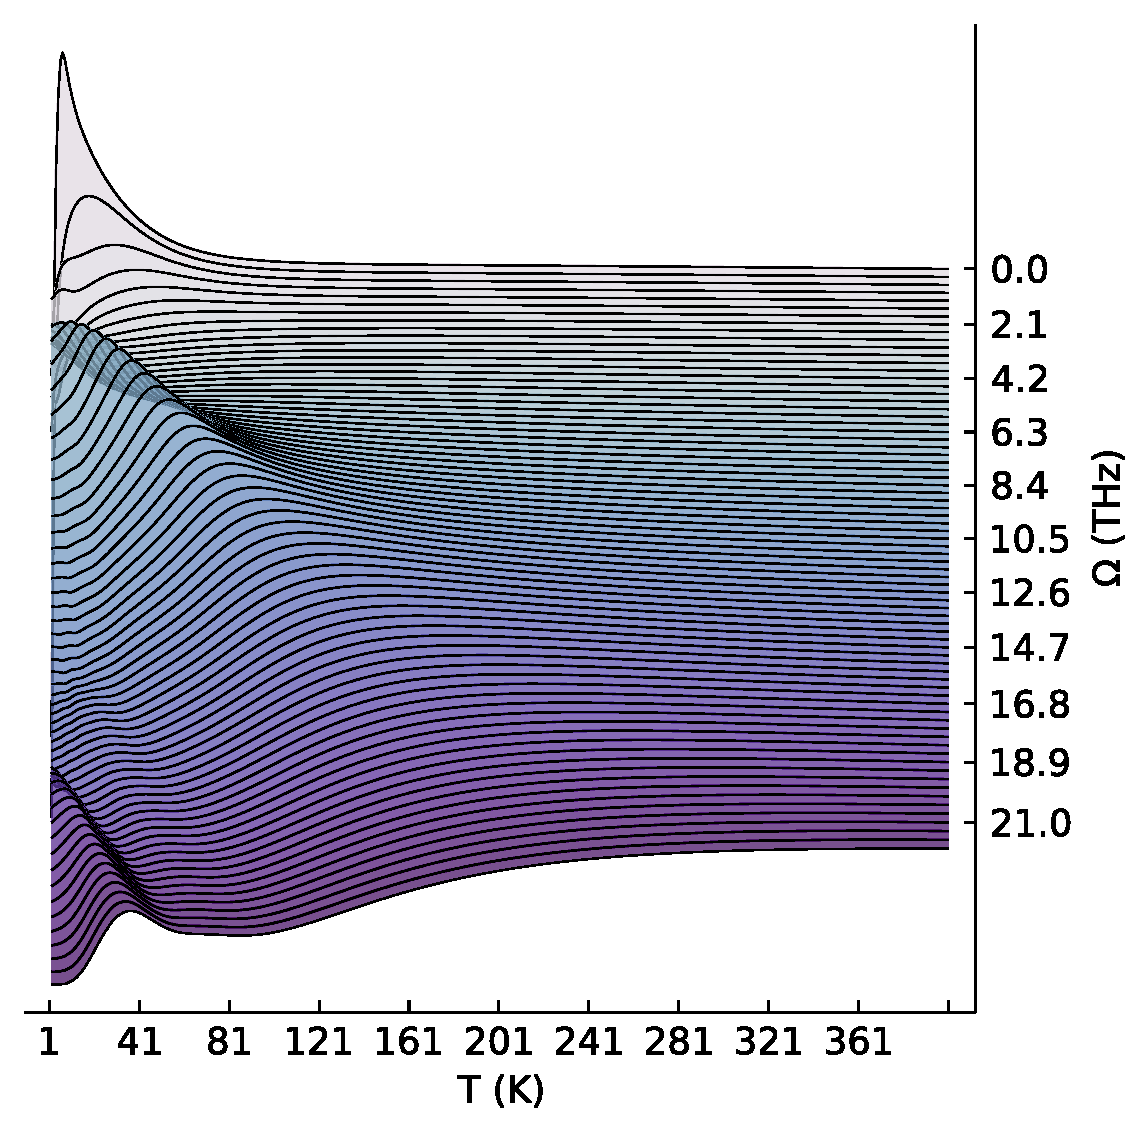
\includegraphics[width=.9\textwidth]{chapters/frohlich/figures/multi_plot_freq_real.pdf}
\end{subfigure}%
\begin{subfigure}[t]{0.01\textwidth}
    \vspace*{-7.5cm}\textbf{b}
  \end{subfigure}
\begin{subfigure}[b]{.58\textwidth}
\centering
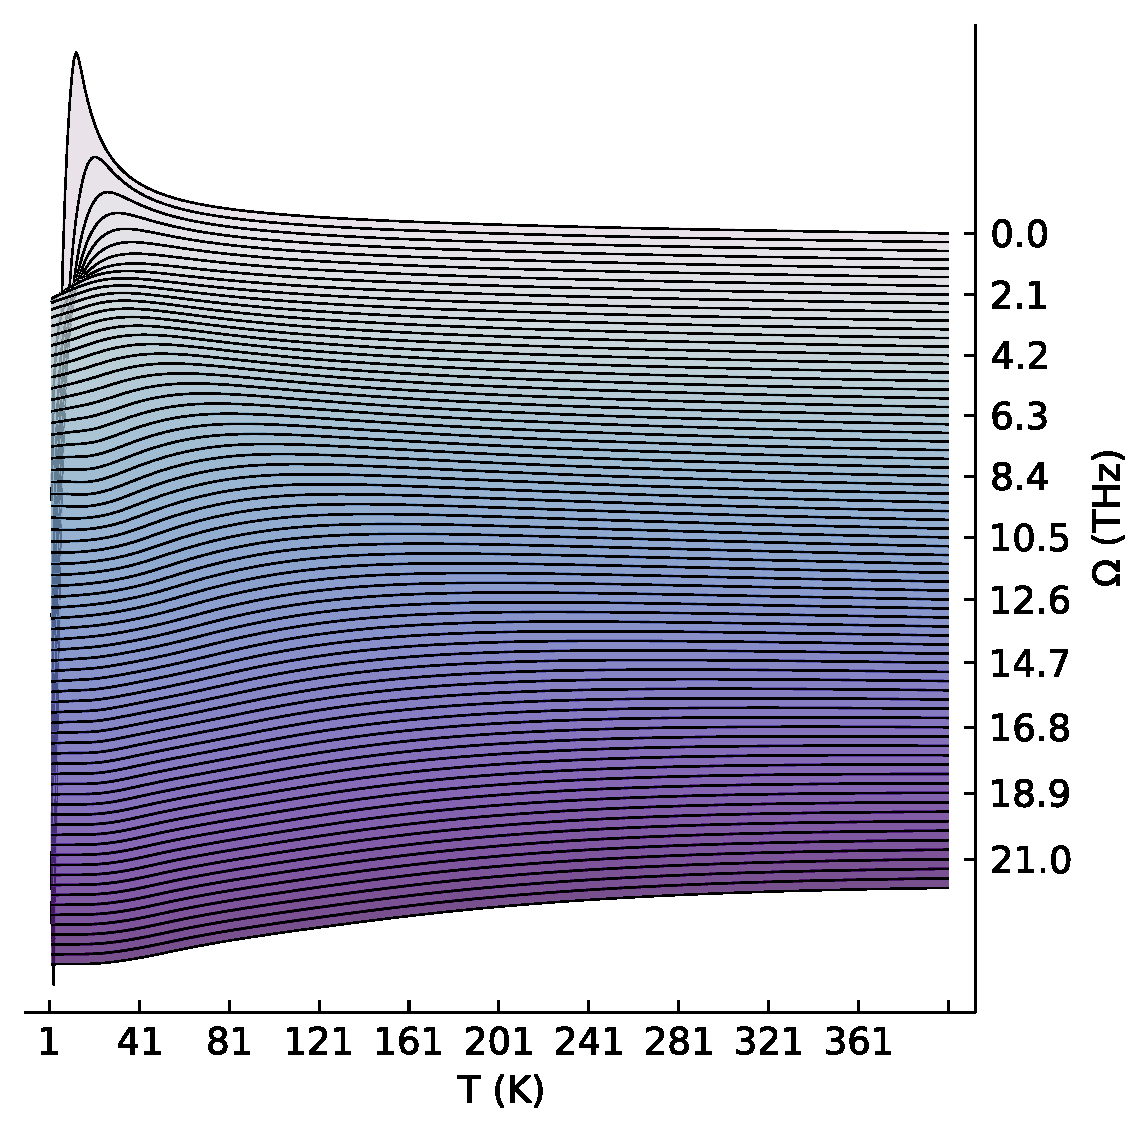
\includegraphics[width=.9\textwidth]{chapters/frohlich/figures/A_plot_freq_real.pdf}
\end{subfigure}%
}\\
\makebox[\linewidth][c]{%
\begin{subfigure}[t]{0.01\textwidth}
    \vspace*{-7.5cm}\textbf{c}
  \end{subfigure}%
\begin{subfigure}[b]{.58\textwidth}
\centering
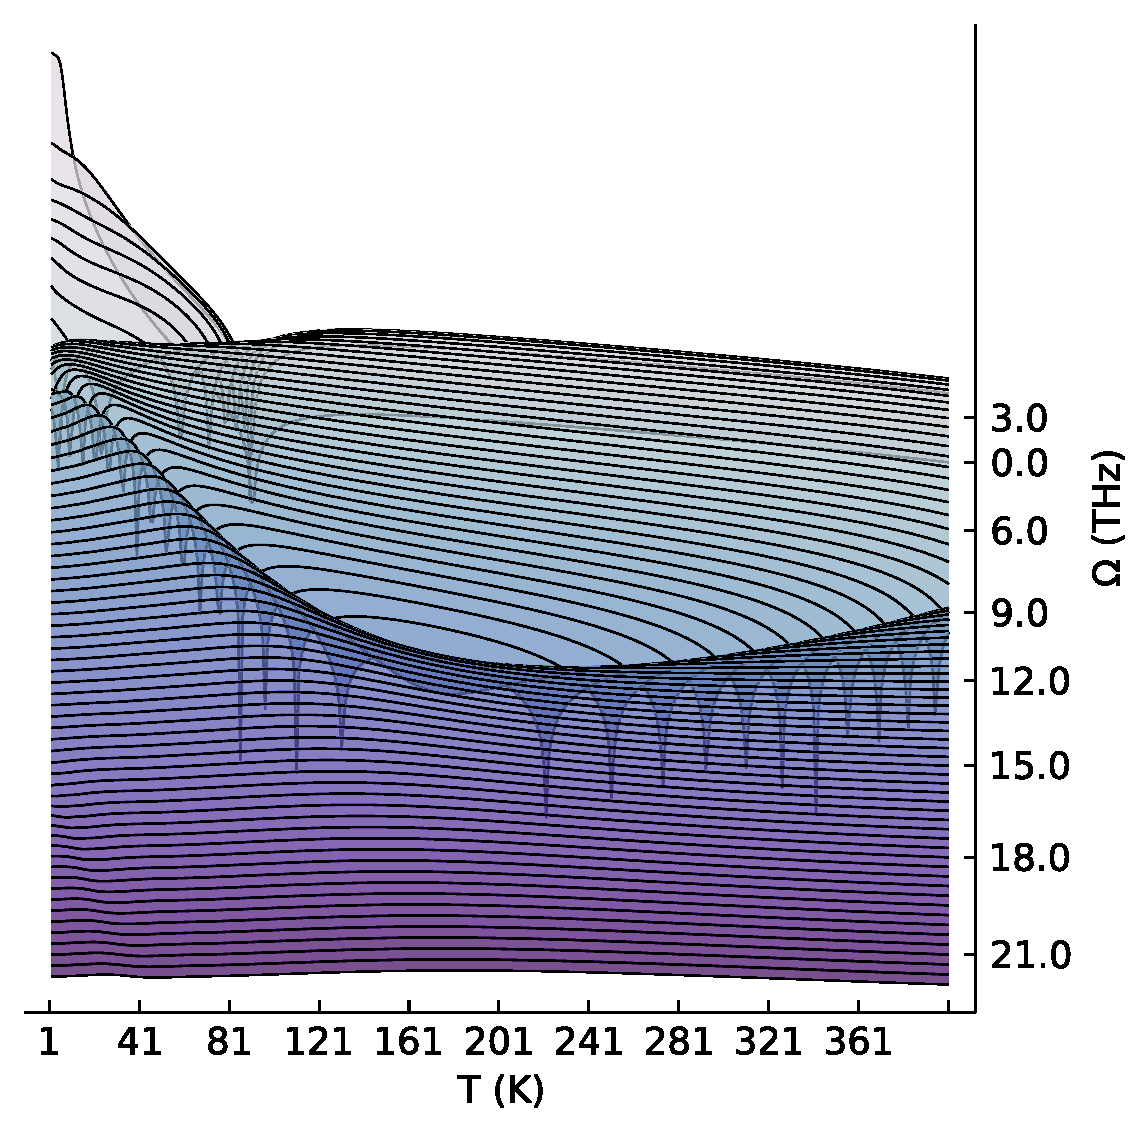
\includegraphics[width=.9\textwidth]{chapters/frohlich/figures/multi_plot_freq_imag.pdf}
\end{subfigure}%
\begin{subfigure}[t]{0.01\textwidth}
    \vspace*{-7.5cm}\textbf{d}
  \end{subfigure}%
\begin{subfigure}[b]{.58\textwidth}
\centering
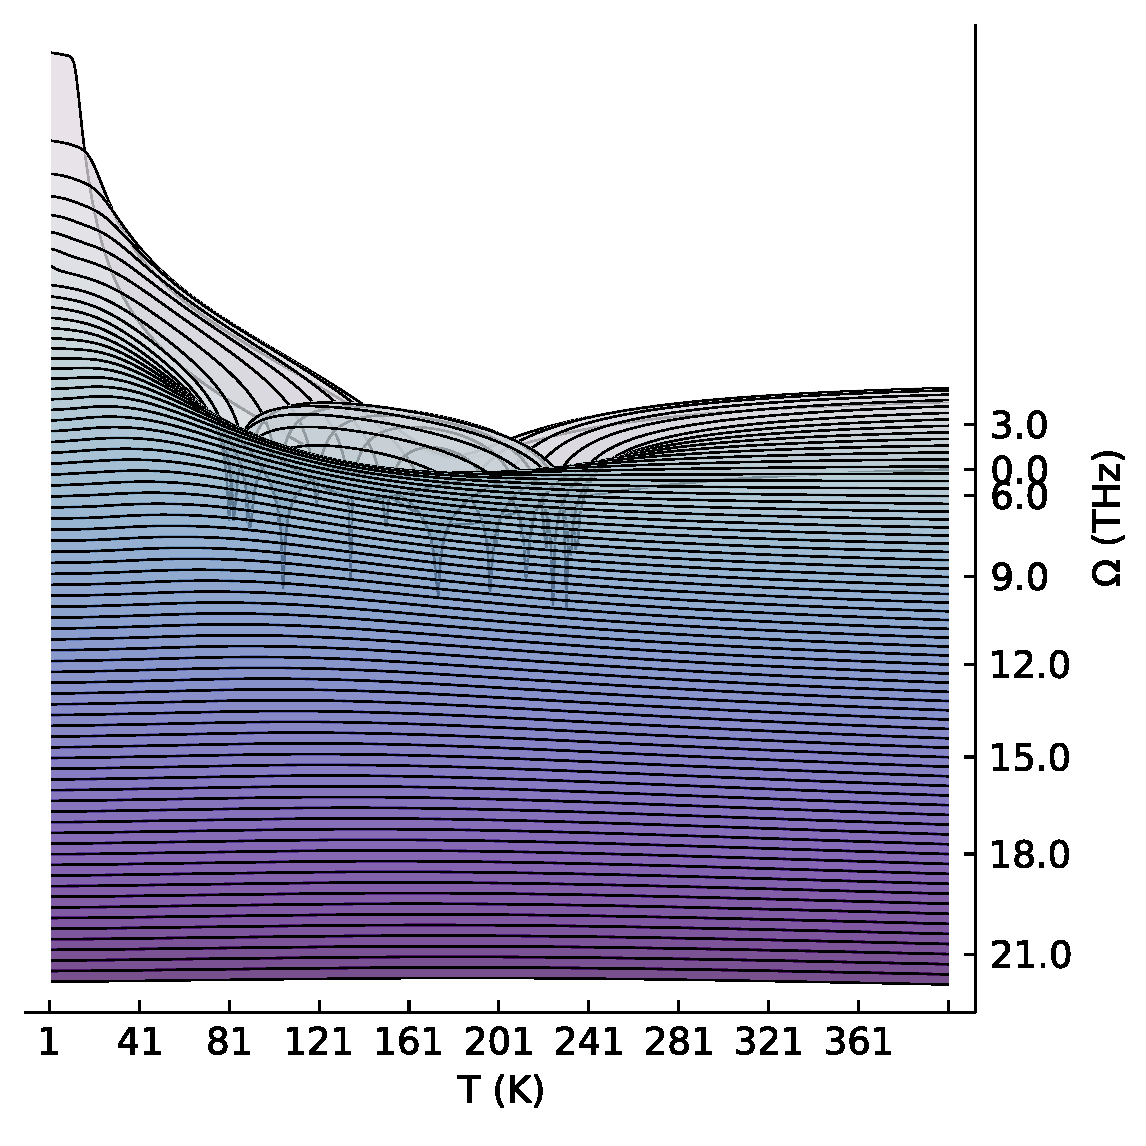
\includegraphics[width=.9\textwidth]{chapters/frohlich/figures/A_plot_freq_imag.pdf}
\end{subfigure}%
}
\makebox[\linewidth][c]{%
\begin{subfigure}[t]{0.01\textwidth}
    \vspace*{-7.5cm}\textbf{e}
  \end{subfigure}%
\begin{subfigure}[b]{.58\textwidth}
\centering
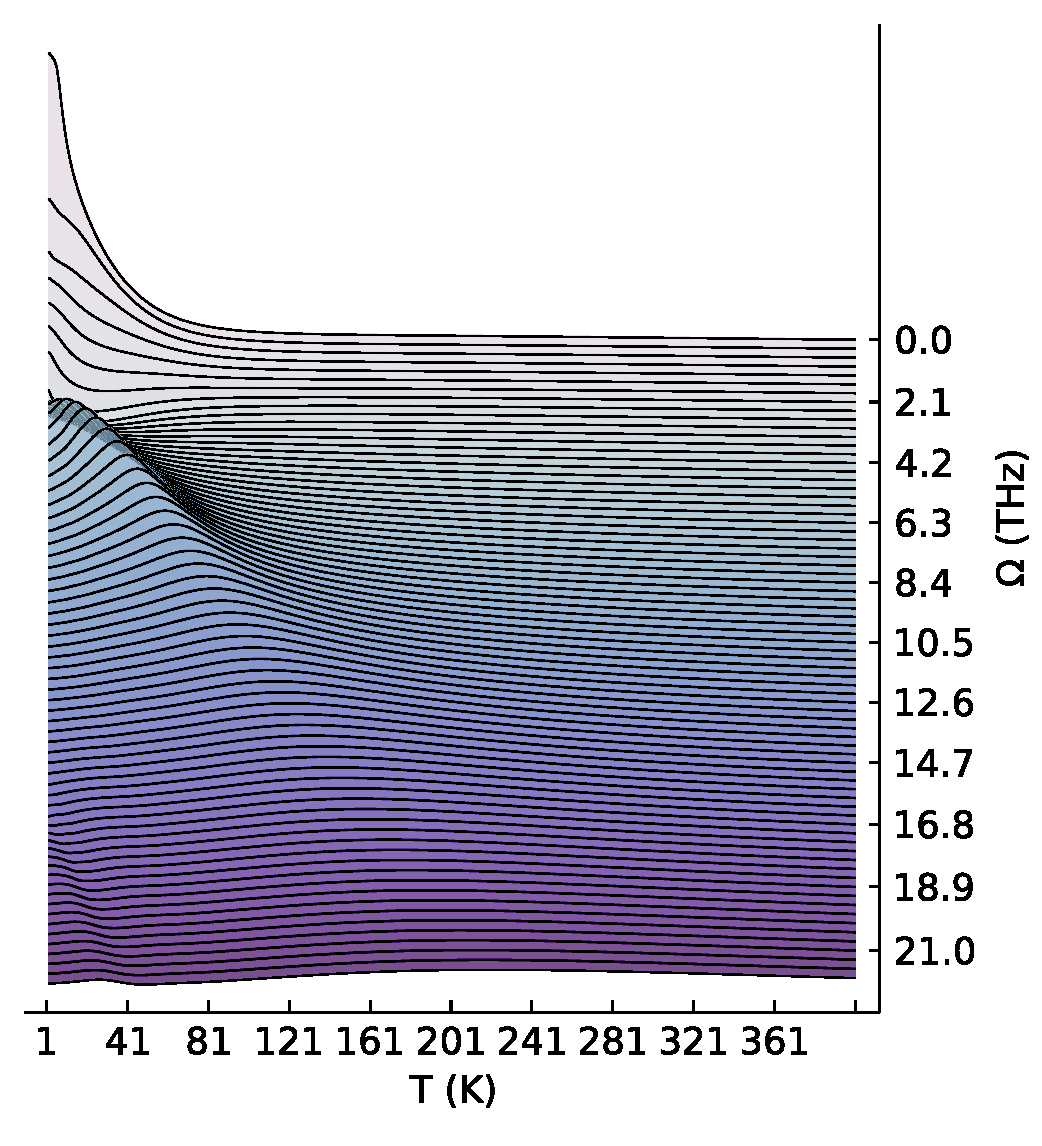
\includegraphics[width=.9\textwidth]{chapters/frohlich/figures/multi_plot_freq_abs.pdf}
\end{subfigure}%
\begin{subfigure}[t]{0.01\textwidth}
    \vspace*{-7.5cm}\textbf{f}
  \end{subfigure}%
\begin{subfigure}[b]{.58\textwidth}
\centering
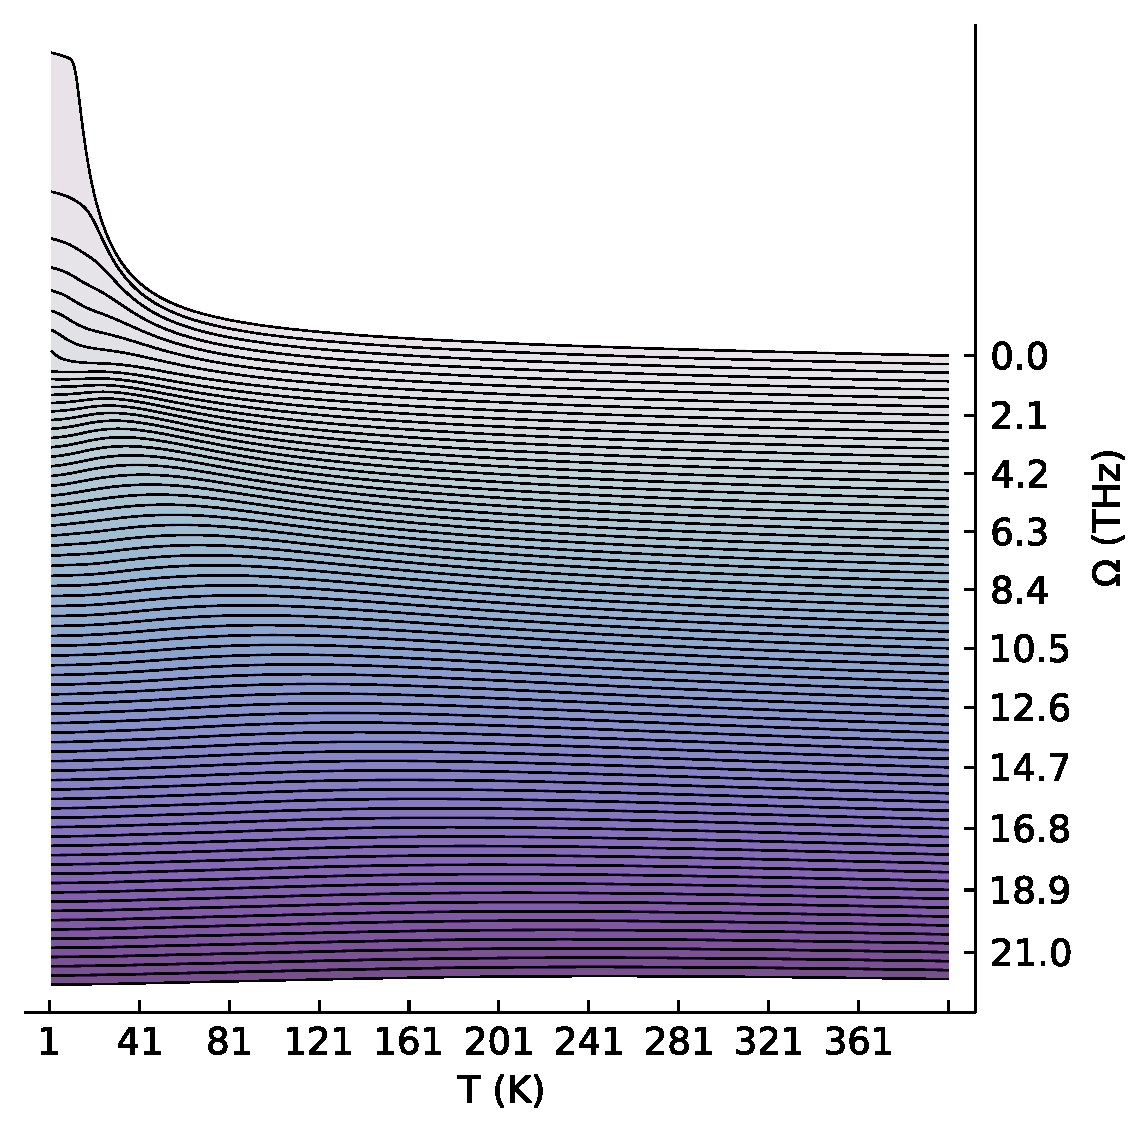
\includegraphics[width=.9\textwidth]{chapters/frohlich/figures/A_plot_freq_abs.pdf}
\end{subfigure}%
}
\caption{(a) Multiple phonon real conductivity. (b) A scheme real conductivity. (c) Multiple phonon imaginary conductivity. (d) A scheme imaginary conductivity. (e) Multiple phonon absolute conductivity. (f) A scheme absolute conductivity.}
\end{figure}

\subsection{Modelling terahertz spectroscopy unveiled polaron photoconductivity dynamics in Metal-Halide Perovskites}

\begin{figure}[t]
\makebox[\linewidth][c]{%
\begin{subfigure}[b]{.6\textwidth}
\centering
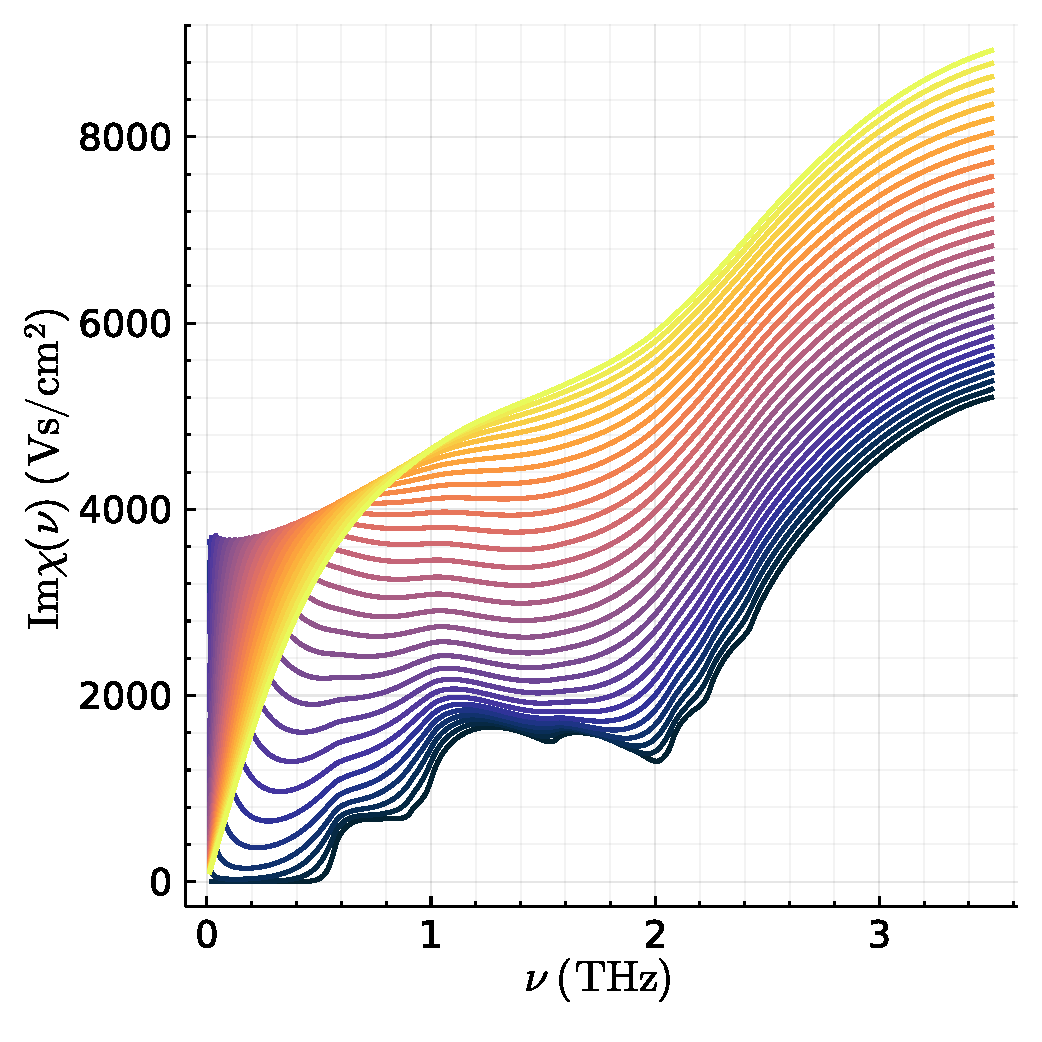
\includegraphics[width=.9\textwidth]{chapters/frohlich/figures/zero_mem.pdf}
\end{subfigure}%
\begin{subfigure}[b]{.6\textwidth}
\centering
\includegraphics[width=.9\textwidth]{chapters/frohlich/figures/zero_conduct.pdf}
\end{subfigure}%
}
\caption{(left): The imaginary part of the multiple phonon mode memory function in Eq. (\ref{eqn:multi_memory}) evaluated for MAPbI$_3$. (right): The real part of the multiple phonon mode complex conductivity (i.e. mobility) in Eq. (\ref{eqn:freq_dep_mobility}) evaluated for MAPbI$_3$. These are calculated for the phonon modes listed in Table 1. The reduced thermodynamic beta $\beta_j = \hbar \omega_j / (k_B T)$ is evaluated for temperatures $T = 1$ K (black curves) to $T = 30$ K (yellow curves).}
\label{fig:athermal_thz}
\end{figure}

Recently, we used used ultrafast visible pump-infrared push-terahertz probe spectroscopy to measure the real-time photo-conductivity of methyl-ammonium lead iodide in~\cite{zheng_multipulse_2021}. In this paper, I provided my multiple phonon mode mobility, applied to the $15$ modes of MAPbI$_3$ in Table 1, to model the complex conductivity and compare the results to the photo-conductivity measurements. 

\begin{figure}[t]
\makebox[\linewidth][c]{%
\begin{subfigure}[b]{.6\textwidth}
\centering
\includegraphics[width=1\textwidth]{chapters/frohlich/figures/thz_plot.pdf}
\end{subfigure}
}
\caption{Terahertz photo-conductivity spectra obtained from a visible pump-IR push-THz probe measurement in~\cite{zheng_multipulse_2021}. The plot shows the real (solid markers) and imaginary (hollow markers) parts of the complex conductivity in MAPbI$_3$. The blue, black and green dashed-lines show before, at and after the arrival of the push pulse, respectively.}
\label{fig:thzplot}
\end{figure}

In Figure \ref{fig:athermal_thz} I provide the low-temperature ($T = 1$ 
K to $T = 30$ K) results of the imaginary component of the memory function $\text{Im}\chi(\nu)$ (left) and the real part of the complex conductivity $\text{Re}\sigma(\nu)$ (right). These have peaks that occur around the frequencies $0.60$ THz, $1.25$ THz and $1.75$ THz, as well as a very broad peak that starts around $2.00$ THz that seems to have extra peaks underlying it to give the appearance of oscillations around $2.15$ THz and $2.25$ THz. 

From Figures \ref{fig:multicontour} and \ref{fig:multiridge} we see that the broad peak is the last feature which decays away at higher frequencies. The broad peak has a maximum around $3.00$ THz at $T = 1$, which flattens and shifts to higher frequencies at higher temperatures where it becomes the only remaining feature. This is to be compared to the photo-conductivity measurements shown in Figure \ref{fig:thzplot}, where the real component maxima occur around the frequencies $1.25$ THz and $2.25$ THz, with a shoulder occur on the side of the $1.25$ THz peak around $0.60$ THz. The shoulder and $1.25$ THz peak seem to be in agreement with the multiple phonon model, however the broader peak, whilst roughly around the right frequency of $2.25$ THz, is far broader and prominent in the theoretical model compared to the photo-conductivity measurements. 

One thing to note is the apparent temperature differences between the multiple phonon model and the experiment. In the multiple phonon model, the one-phonon peaks associated with each phonon mode only appear at very low-temperatures and are quickly washed out as the temperature increases until at around $T > 10$ K, only the broad peak around $3.00$ Thz remains. In the multiple phonon theory, it is assumed that the electron and phonon thermal-bath are at thermal equilibrium. However, in the experiment the electron(s) is definitely not at thermal equilibrium and is very hot.

\begin{figure}[h]
\makebox[\linewidth][c]{%
\begin{subfigure}[b]{.6\textwidth}
\centering
\includegraphics[width=.9\textwidth]{chapters/frohlich/figures/multi_contour_real_chi.pdf}
\end{subfigure}%
\begin{subfigure}[b]{.6\textwidth}
\centering
\includegraphics[width=.9\textwidth]{chapters/frohlich/figures/multi_contour_real_0.pdf}
\end{subfigure}%
}
\caption{Contour plots for (left): The imaginary part of the multiple phonon mode memory function (\ref{eqn:multi_memory}) evaluated for MAPbI$_3$. (right): The real part of the multiple phonon mode complex conductivity (\ref{eqn:freq_dep_mobility}) evaluated for MAPbI$_3$. Here the temperature axis is log-scaled and ranges from $T = 1$ K to $T = 400$ K and frequency zoomed in onto the range $\nu = 0$ THz to $\nu = 3.5$ THz.}
\label{fig:thermal_thz}
\end{figure}

\begin{figure}[t]
\makebox[\linewidth][c]{%
\begin{subfigure}[b]{.6\textwidth}
\centering
\includegraphics[width=.9\textwidth]{chapters/frohlich/figures/ff_zpr.pdf}
\end{subfigure}%
\begin{subfigure}[b]{.6\textwidth}
\centering
\includegraphics[width=.9\textwidth]{chapters/frohlich/figures/ff_emass.pdf}
\end{subfigure}%
}
\caption{Both figures are taken from~\cite{guster_frohlich_2021}. (left): The relative differences between the ground-state energy of the polaron determined using perturbation theory (which fully accounts for any anisotropy) and the Feynman variational approach (using my approximate treatment of anisotropy). (right): The relative difference between the effective masses determined using perturbation theory and the Feynman variational approach (again only approximately accounting for anisotropy). $m^*_{P, iso}$ is the isotropic effective mass, $m^*_{P, \perp}$ and $m^*_{P, z}$ are the in-plane and out-of-plane polaron effective masses.}
\label{fig:anisotropy}
\end{figure}

\subsection{Fr\"ohlich polaron effective mass and localisation length in cubic materials:  degenerate and anisotropic electronic bands}

In~\cite{guster_frohlich_2021}, we investigate the polaron effective mass, radius and ground-state energy that arise from a generalised Fr\"ohlich Hamiltonian that incorporates degenerate bands with anisotropy and multiple phonon branches. These polaron properties are calculated for 20 cubic materials (including II-VI compounds: CdS, CdSe, CdTe, ZnS, ZnSe, ZnTe; III-V compounds: AlAs, AlSb, AlP, BAs, BN, GaAs, GaN, GaP; oxides: BaO, CaO, Li$_2$O, MgO, SrO; and SiC) using the lowest order of perturbation theory and the strong coupling limit. \newline

\noindent In the non-degenerate case, I provide a na\"ive extension of Feynman's path integral approach to include anisotropic effective band masses which is used as a point of comparison with the full perturbative treatment for characterising the polaron in the weak-coupling limit (c.f. section IIb in~\cite{guster_frohlich_2021} and subsection 3.8 of this chapter). From Figure \ref{fig:anisotropy} (left) we see that the variational approach gives a lower estimate for the ground-state compared to the perturbative result for both isotropic (up to $2.5$\% lower) and anisotropic (up to $17.5$\% lower) materials. In Figure \ref{fig:anisotropy} (right), we have the relative difference in polaron effective mass between the two approaches. The largest difference is found in materials that, within the Fr\"ohlich approach, are found in~\cite{guster_frohlich_2021} to be at the continuum limit breakdown where the discrete nature of the lattice cannot be ignored. These materials include BaO, CaO, SrO and, to a lesser extent, Li$_2$O. In both the anisostropic and isotropic cases the relative difference increases with polaron effective mass, and the in-plane and out-of-plane effective mass differences seem to diverge. This sudden increase in the relative difference is associated with a breakdown limit around $\alpha = 6$ in the perturbative approach for determining the polaron effective mass.

\section{Discussion}

Path integration is a powerful tool for finding accurate approximate solutions to the free energy of the polaron model and for describing the response of the polaron. The main result of my project so far has been the extension of the path integral approach to the polaron to explicitly include multiple phonon modes, and using the previously established techniques to make predictions of the complex conductivity. I will discuss here my interpretation of the results of my new multiple phonon model and the comparisons to Hellwarth's effective frequency model. Additionally, I will discuss the result of the application of my model to terahertz conductivity measurements of MAPbI$_3$, as well as the result of modelling anisotropy in materials in two recent papers. 

\subsection{Predictions from FHIP and DSG for the complex mobility}

The first thing to discuss is what one might expect to get from including multiple phonon modes given the result of a single mode. In~\cite{feynman_mobility_1962} and~\cite{devreese_optical_1972}, the predicted imaginary component of the memory function $\text{Im}\chi(\nu)$ and real component of the complex conductivity $\text{Re}\sigma(\nu)$ always included an initial peak starting sharply at the phonon mode frequency when at zero temperature. This is the only peak present for lower values of the electron-phonon coupling with $\alpha < 4.5$. It is only at couplings stronger than this that extra oscillatory peaks arise at multiples of the phonon mode frequency multiplied by the value of the variational parameter $\omega_{LO} \times v$. 

This new frequency, $\omega_{LO} \times v$, can be thought of as the polaron frequency, and so these extra peaks would be identified as polaron excitations. The first peak also develops a bit of an initial shoulder followed by a tall, sharp peak. In DSG they identified these peaks as an initial one-phonon peak at $\Omega = \omega_{LO}$ at lower $\alpha$s. As $\alpha$ increases, extra oscillator strength is added due to transitions to final states where lattice adaption to excited electronic configurations (Relaxed Excited States or RES) has occurred. A further increase in coupling produces a separation of the one-phonon and RES states. Eventually a side-band structure forms, which leads to a broad Frank-Condon (FC) peak that is a superposition of multiphonon sidebands and is less pronounced than the RES peak. 

At strong coupling the conductivity becomes very `structured' and it is hard to identify clear features. The extra `structure' is likely due to the breakdown of the Fr\"ohlich model in the strong-coupling limit, where the linewidth of the FC peak becomes smaller than $\omega_{LO}$. This violates the lifetime of $1 / \omega_{LO}$ derived from uncertainty relations and signals the breakdown of the Fr\"ohlich model at strong coupling due to the continuum approximation; the breakdown is not due to the FHIP approximation. 

Devreese has used an operator based theory \cite{Devreese2001} for the strong coupling limit that agrees well with Diagrammatic Monte Carlo data. This would explain the apparent breakdown of the conductivity in the $\alpha = 9$ plots. 

\subsection{Comparison of the multiple phonon and effective frequency mobilities}

I found that regardless of coupling strength, all peaks broaden, flatten and blue-shift to high frequencies as the temperature increases. Eventually, for temperatures greater than $100$ K, we recover a Drude-like response with all the oscillations dampened away. 

Including multiple phonon modes would superimposed multiple peaks in the memory function $\chi(\nu)$ (Eq. (\ref{eqn:multi_memory})), each starting at each of the respective phonon mode frequencies. The magnitude of these peaks would depend on the relative contributions of the modes to the overall electron-phonon coupling. The coupling would be proportional to the infrared activity of each respective mode. 

Comparing the memory function and the complex conductivity in DSG, we expect that the complex conductivity would possess similar structure to the memory function, with peaks starting at each respective phonon mode frequency. However, the overall structure is not the result of a straight forward superposition and instead involves the reciprocal of the sum over phonon modes as seen from Eq. (\ref{eqn:freq_dep_mobility}). Since the majority of real materials have Fr\"ohlich $\alpha$ values less than $4.5$, we would not expect to see any additional oscillations at higher frequencies corresponding to polaron excitations. Any extra peaks would be due to some combination of the many one-phonon peaks from each mode. 

From Figure $9$, we see that the multiple phonon mode mobility $9a$ has a very similar form to the single effective mode mobility $9b$, with one primarily broad peak starting around the Hellwarth and Biaggio effective frequency $2.03$ THz. This broad peak in the multiple phonon mobility is likely a result of the combined contributions from the $2.080$ THz, $2.249$ THz and $2.438$ THz modes which, from Table 1, we can see have the first, second and fourth largest contributions to the decomposed $\alpha_j$ parameter. Due to the combination of these three modes to form the broad peak, the multiple phonon mobility shows extra detail in the broad peak. The extra detail appears as a small initial oscillation at the start of the peak as seen in Figure $10$. 

Below $2$ THz in Figure $9$, the multiple phonon mobility possesses three main extra peaks that do not appear in the effective frequency mobility. These peaks are sharper than the broad peak and begin around $0.60$ THz, $1.00$ THz and $1.50$ THz. From Table 1 we see that the $0.574$ THz mode has the third largest contribution to the decomposed alpha parameter $\alpha_j$ and is likely the source of the first sharp peak around $0.60$ THz. The cluster of modes ranging from $0.801$ THz to $1.019$ THz are probably the source of the peak that starts around $1.00$ THz. Finally, the $1.567$ THz mode has a comparatively intermediate contribution to $\alpha_j$ and is likely the source of the small peak around $1.50$ THz, which appears more like a shoulder off of the back of the $1.00$ THz peak.

\subsection{Comparison of the multiple phonon mobility with THz photo-conductivity data}

From the photo-conductivity measurements, the two strong resonances around $1.25$ THz and $2.25$ THz are attributed to two groups of optical phonon modes associated with the bending and stretching of the Pb-I bond in MAPbI$_3$. In~\cite{zheng_multipulse_2021} we conclude that the origin of the non-Drude-like spectral response cannot be explained primarily by non-polaronic free carriers alone, and will likely require further investigation with non-equilibrium response theories. Nonetheless, the dominant effect of reducing the conductivity is attributed to the excitation of the electronic states as well as an interplay between the polaron and surrounding lattice that result in the peaks in the conductivity. The scenario described is one where the underlying phonons, that are strongly coupled to the charge-carriers and are a part of polaron formation, are heated by the carriers as the carriers cool. This occurs before the heat can be dissipated from these strongly coupled phonon modes scattering into non-coupled phonons (that are not involved in the polaron formation). 

Comparison with the multiple mode conductivity in Figure (\ref{fig:athermal_thz}) leads to reasonable qualitative agreements where the main resonances in the predicted response seem to align with the observed response. The $2.25$ THz peak is far broader in the theory, but it should be noted that the form the predicted response takes is sensitive to the modes provided, so that alternative measured/predicted values of phonon mode frequencies and infrared activities would alter the predicted spectral response. 

The best agreement with the measurements occurs when the effective temperature of the system is near to zero. This suggests that the sub-picosecond time scale of the THz probe measurement corresponds to a pre-thermal equilibrium mobility regime. It is not entirely clear how this can be established qualitatively and will the subject of further investigations. 

The multiple phonon mode model has the capability of involving more than just two $v$ and $w$ variational parameters, which would correspond to have more fictitious harmonic oscillators coupled to the charge-carrier in the model system. It would be interesting to investigate how including more harmonic oscillators changes the predicted response. It may be that matching the number of fictitious oscillators to the number of strongly coupled phonon modes would make more accurate predictions. However, I have not been able to investigate this yet due to issues with computational convergence of the variational expression in Eq. (\ref{eqn:multi_feynman_jensen}).

\subsection{Comparison of the variational and full perturbative approaches for modelling anisotropy}

From~\cite{guster_frohlich_2021} and shown in Figure (\ref{fig:anisotropy}), we find reasonable agreement in the weak-coupling regime between the proper perturbative treatment of anisotropy in the Fr\"ohlich model and the naive inclusion of anisotropy in the athermal Feynman path integral model. The best agreement is clearly for the inherently isotropic materials, with poorer agreement for the more anisotropic materials, although the difference is minor. For the anisotropic materials, the Feynman approach seems to over-estimate the in-plane effective masses compared to the full perturbative approach. This is likely due to the improper treatment of the anisotropic mass in the variational principle when determining the variational parameters that correspond to the in- and out-of-plane directions. This would explain the underestimate of the ground-state energy by the Feynman approach too, although it should be noted that the Feynman approach will always be expected to predict a lower ground-state energy than the perturbative approach. 

I recently found a 1982 paper by Peeters and Devreese \cite{Devreese1982} where they extend Feynman's polaron theory to account for anisotropy of the effective electron-phonon interaction under the influence of a perturbing magnetic field. The extended free energy variational principle in \cite{Devreese1982} would give the foundation for a proper treatment of anisotropic in the path integral approach to obtaining polaron effective masses. When discussing comparisons between the Feynman and perturbative approaches, we found that defining a polaron radius can be quite ambiguous. It would be useful to find a formal definition for the polaron radius to help with comparison between difference theoretical approaches. One way to do this may be to look at the maxima of the dynamic structure factor which may help define an effective polaron radius. In terms of the path integral model, the dynamic stucture factor is found by evaluating $\langle \exp(i \vb{k} \cdot [\vb{r}_{el}(t) - \vb{r}_{el}(0)]) \rangle_{S_0}$ Eq. ((\ref{eqn:S})) as indicated in \cite{Devreese2001} and \cite{Devreesetwo}.